\documentclass[11pt]{article}
\usepackage[margin=1in]{geometry}
\usepackage[T1]{fontenc}\usepackage{lmodern,microtype,caption,longtable}
\captionsetup{font=small,labelfont=bf,skip=5pt}
\DeclareCaptionFont{qkicompact}{\fontsize{9}{10}\selectfont}
\usepackage{amsmath,amssymb,graphicx,booktabs,array,natbib,float}
\usepackage[colorlinks=true,allcolors=blue]{hyperref}
\graphicspath{{figures/}}
\setlength{\emergencystretch}{1em}
\title{Supplementary Methods, Tables, Figures and Data\\for CARBON: a conservation-aware framework for\\base-resolution RBP binding profile prediction}
\author{Bin Wu\thanks{ORCID 0009-0002-6711-7230, College of Artificial Intelligence, Jilin University}}
\date{}
\begin{document}
\renewcommand{\thefigure}{S\arabic{figure}}
\renewcommand{\thetable}{S\arabic{table}}
\maketitle

\section*{Scope}

This supplement specifies the benchmark population, evaluation definitions, architecture, training partitions, motif analysis, conservation localization and frozen-checkpoint perturbation analyses. It distinguishes pooled task correlations from within-window paired effects and defines the aggregation and resampling units used in each figure. The bulk perturbation experiment used existing checkpoints on a deterministically sampled chromosome-8/15 subset without new training or hyperparameter search. A separate two-task training-seed sensitivity analysis is reported in S1.16. S1.17 specifies the three-seed native repeated-core architectural comparison, and S1.18 specifies external word-preference validation and exploratory sequence-order interventions. S1.19 documents motif-reference provenance, and S1.20 specifies the natural-variant extension and exploratory conservation associations. Main Figures~4 and 5 combine these analyses; complementary conservation and perturbation analyses appear in Figures~S12 and S13.

Supplementary Data S1--S10 contain the original benchmark and analysis summaries. S11--S14 contain bulk perturbation, RBP-level conservation and numerical reconstruction summaries. S15--S20 provide the conditional conservation, factorial sequence-response, published ASB and benchmark-extrema records. The accompanying experiment records identify selected source rows and input/checkpoint hashes, and provide the per-window endpoints used to reconstruct the retained analyses. S22 and S23 contain the complete native-allocation and external-preference packages. S24 documents motif-reference sources and comparisons; S25 supplies natural variants, official allele-level annotations, frozen model outputs and descriptive association analyses.

\section{Supplementary Methods}

\subsection*{S1.1 Six evaluation metrics and their exact decision thresholds}

The definitions below apply to the CARBON and iDeepB evaluators used for the reported scores, including CARBON ablations. They do not describe the historical RBPNet evaluator, whose different peak mask and tied-rank handling are specified in S1.3. Task-name and chromosome matching do not establish an identical evaluated window set. Three metric groups are retained.

\paragraph{Correlation metrics.} For a task $t$ with test windows $w = 1,\dots,W_t$, let $\hat{\mathbf{v}}_t$ be the concatenation of all predicted values of the task's test windows and $\mathbf{v}_t$ the identically concatenated observed values, so that $|\hat{\mathbf{v}}_t| = |\mathbf{v}_t| = W_t \cdot L$ with $L = 101$.

\begin{align}
\text{Mean PCC}_t &= r_{\mathrm{Pearson}}\!\left(\hat{\mathbf{v}}_t,\ \mathbf{v}_t\right),\\
\text{Spearman}_t &= r_{\mathrm{Spearman}}\!\left(\hat{\mathbf{v}}_t,\ \mathbf{v}_t\right).
\end{align}

\textbf{The field name \texttt{Mean\_PCC} is retained for traceability to the evaluation code, but it does not denote the arithmetic mean of per-window Pearson correlations.} It is the Pearson correlation of the flattened task-level vectors defined above, i.e.\ it is a per-task quantity that is only later averaged across tasks. The Spearman correlation is computed on exactly the same pair of flattened task-level vectors. Reported table values are unweighted means of the per-task quantities across tasks.

\paragraph{Signal-level metrics.} Signal AUROC and Signal AP were computed from the same flattened per-task vectors. A position was treated as a positive if its observed value exceeded the task-specific median of the flattened observed vector, and the corresponding flattened prediction was used as the score. Positions equal to the threshold were negative because the code uses a strict greater-than comparison; the threshold definition is therefore \emph{task-specific} and \emph{flattened}, not per-window and not global across tasks.

\paragraph{Peak-level metrics.} Peak AUROC and Peak AP were computed from contiguous non-zero observed segments. A segment was accepted as a peak region when it satisfied all of:

\begin{itemize}
\item minimum segment length of 1 base,
\item maximum signal within the segment at least 2 counts, or segment sum at least 2 counts.
\end{itemize}

The evaluator was therefore invoked with a maximum-signal / total-signal / minimum-length argument triple of $(2,\,2,\,1)$. The peak rule was applied only to the peak-level metrics; signal-level metrics used the median rule described above, and correlation metrics used no thresholding at all. The evaluator marks individual bases in qualifying segments and scores those bases; it does not evaluate peak objects. Segment detection runs on the flattened vector without a boundary reset between consecutive windows, so adjacent terminal non-zero values can be joined across window boundaries. This convention is retained in the frozen metrics. The Signal and Peak metrics can have very similar labels and values and are not independent evidence.

\paragraph{Paired comparisons.} Paired model and ablation comparisons used two-sided paired Wilcoxon signed-rank tests on task-level values, without multiple-comparison correction. They are reported as exploratory. No benchmark-wide repeated-training uncertainty was estimated; the separate two-task check in S1.16 does not supply such an estimate. The original tests treat task records as paired units without fully accounting for shared RBP and genomic context; their nominal $p$ values document these exploratory comparisons and do not support confirmatory biological inference.

\subsection*{S1.2 Task population and partition provenance}

\paragraph{Upstream record construction.}
The study starts from previously generated eCLIP records in the iDeepB processing collection. Archived code pools treatment BAMs and input BAMs separately before extracting strand-specific read-end signal. The retained examples share GENCODE v29 transcript intervals, the GRCh38.p12 reference, \texttt{samFlag=128}, 101-nt windows, \texttt{padding\_Mode=Random} and \texttt{signalGap=0}. Count filtering, Poisson testing and correction differ between versions. The \texttt{achieveV2} AARS configuration records \texttt{min\_Count=4}, \texttt{sum\_Count=12}, \texttt{poisson\_Test=None}, \texttt{correction=1} and \texttt{min\_pval=0.01} (inactive when the test is disabled). The retained Archive 4 AKAP1 and AGGF1 YAML configurations instead record \texttt{min\_Count=0}, \texttt{sum\_Count=0}, \texttt{poisson\_Test=poissonTest}, \texttt{correction=0} and \texttt{min\_pval=0.05}. The count-selection code uses maximum count \emph{or} total count. These archived configurations are not interchangeable provenance for the full benchmark.

The \texttt{wholeOverlap=whole} rule requires the entire segment to overlap a transcript interval on the same strand (\texttt{s=True}, \texttt{f=1.0}). For short segments, random padding is allocated within available transcript boundaries. Long segments are extended to an integer multiple of 101 and split into successive records; a peak is therefore not necessarily centred. The original invocation, count-filter choice and padding records have not been linked completely for every task. We use the recorded sequence/interval/observed vectors as the inherited input population and do not assign one upstream count threshold to all 222 tasks. The subsequent five-channel converter filters N-containing or incomplete records, retrieves coordinate-matched PhyloP, reverses it for minus-strand records and assigns zero to missing values. Stored sequences and intervals define each analysed record. These configurable upstream rules are distinct from the evaluation labels in S1.1.

The benchmark contains 222 tasks covering 150 RBP symbols: 119 K562, 101 HepG2 and two adrenal-gland tasks. Task identifiers combine RBP, cell/tissue context and ENCODE accession. The two tissue tasks are DGCR8 (ENCSR634MFO) and HNRNPU (ENCSR368GER), both from adrenal gland; they are labelled \texttt{other} in the frozen benchmark table and have an empty cell-line field in the conservation summary. Their display category is resolved from the accession-linked tissue metadata. They are not independent biological replicates. The retained benchmark was derived from 225 source tasks; two were omitted for compute budget and one failed processing.

The final training runs used chromosomes 1, 8 and 15 for evaluation, 2, 9 and 16 for validation, and the remaining 16 autosomes for training. However, the earlier 65-trial search used chromosome 1 for training, chromosome 2 for validation and chromosome 3 for evaluation. Command records for all 325 trial--task jobs (65 trials over five tasks), including selected trial 64, have these assignments. The BED-to-HDF5 processing code groups by actual chromosome, so these names do not merely denote abstract split labels.

Chromosome 1 was therefore exposed during development of the configuration later assessed on the final evaluation partition. The final training and validation files are separate from that partition, but the partition is not untouched by the full development process. The benchmark reports these measured scores. The perturbation experiment evaluates existing checkpoints on chromosomes 8 and 15, excluded from the recorded early search and final training/validation. These chromosomes were already included in the earlier benchmark, so this restriction does not constitute a new independent validation. A new partition excluded from the whole search and development process is needed to resolve this limitation. Chromosome separation also does not remove homologous sequence across chromosomes; no sequence-identity filter was used.

\subsection*{S1.3 Comparator alignment and prediction semantics}

The archived benchmark table joins three independently generated task-summary files; it does not rescore all predictions with one evaluator. Reconstruction from the evaluation code reproduces all 3,996 displayed numerical entries from the 666 original task summaries, but identifies incompatible output and metric definitions. This numerical correspondence does not establish that the outputs or metrics are comparable.

\begin{center}\small
\begin{tabular}{@{}p{.16\linewidth}p{.35\linewidth}p{.41\linewidth}@{}}
\toprule
Implementation & Scored output & Evaluation and population differences \\
\midrule
CARBON & $\mathbf p\exp(z)$, with target $\log(S+1)$ & Count-like output; sklearn-based ranking metrics and the max-or-sum peak rule in S1.1. Ambiguous sequences are filtered. \\
iDeepB & Direct Treat/Poisson output in the recovered runner; log mode is not enabled & Same metric family as CARBON in the recovered source. Historical per-task invocation linkage still needs consolidation; ambiguous sequences are filtered. \\
RBPNet & Mixed treatment-profile head, softmax-normalised across each 101-nt window & Unit-sum output without a count multiplier; different peak mask and rank implementation. Its converter retains ambiguous-base windows and maps unknown bases to A. \\
\bottomrule
\end{tabular}\end{center}

The RBPNet peak evaluator requires a local maximum of at least two and a qualifying segment sum. Unlike the max-or-sum rule, it excludes a contiguous segment such as $[1,1]$, despite its total of two. Its AUROC/AP routines use individual sorted ranks without standard tie handling. For constant predictions, this can yield AUROC zero or one instead of the correct 0.5. RBPNet's unit-sum window profiles also omit between-window abundance variation that remains in CARBON and iDeepB outputs; pooled correlation and ranking are therefore not matched estimands. The direction or magnitude of changes after corrected evaluation cannot be inferred from the saved summaries.

A common evaluation requires matched genomic windows and observed signal, separate profile-shape and abundance endpoints, and one boundary-aware scorer with standard tie handling. Complete three-model per-window prediction arrays were unavailable. The current standard-path audit identifies 221 CARBON, 219 iDeepB and 222 RBPNet checkpoints. The historical CARBON SERBP1 K562 benchmark checkpoint is missing from its standard path; an available ablation baseline is not established as the same checkpoint. The three missing iDeepB tasks are AKAP1 HepG2, BUD13 HepG2 and SERBP1 K562, with exact accessions retained in the checkpoint inventory. Figure~2, Supplementary Figure~S4 and Table~S1 therefore retain historical implementation summaries without establishing a fair method ranking. The former CARBON identifier \texttt{marcp} remains in source tables.

The FMR1 K562 example in Figure 2h covers hg38 chr1:241850473--241850574 (+). The recovered plotting script reads pooled treatment \texttt{Y} and control \texttt{Y\_ctl}, plots $-|Y|$ and $-|Y_{\mathrm{ctl}}|$ below baseline, and had incorrectly labelled them as ENCODE replicates. The labels are corrected to inverted pooled eCLIP and inverted control signal. These are not independent replicate measurements; the first downward trace repeats the pooled treatment signal. Track-specific scales differ. Full file accessions and the exact historical 101-position prediction arrays remain insufficiently linked to recompute the displayed correlations independently.

\paragraph{Common colour encoding in Figure~2.} All three PCC rings share the same task order and one NPG-light-blue--white--red map over $[-0.1,0.5]$ with a common power contrast ($\gamma=0.65$) around white. White is placed at the pooled median of all 666 scores, 0.2853291903436592. The same continuous map applies to every score; it is not a chance, significance or biological threshold. There is no model-specific normalization or colour map. Panel g uses unstandardized CARBON-minus-comparator scores, with one zero-centered $[-0.12,0.12]$ map across all 2,664 entries. The upper colour-bar extension denotes the 195 values above 0.12; none is below $-0.12$. The outer CARBON ring is wider to aid identification (3.55 mm versus 1.93 mm for each inner model ring); ring width carries no metric value. This colour encoding does not correct unequal output scales or evaluators. Data S20 retains every original value; the current colour function is specified below and in the editable figure source.

For the Figure~2a colour coordinate, let $L=-0.1$, $C=0.2853291903436592$, $U=0.5$ and $\gamma=0.65$. Values are mapped to
\[
t(x)=\begin{cases}
\tfrac12\!\left[1-\big((C-x)/(C-L)\big)^\gamma\right],&L\leq x\leq C,\\
\tfrac12\!\left[1+\big((x-C)/(U-C)\big)^\gamma\right],&C<x\leq U.
\end{cases}
\]
The same monotone function applies to every model, without clipping any of the 666 PCC values. Higher-scoring baseline entries therefore remain red. Data S20 provides the original values and earlier colour encodings; the current display parameters are specified here. Colour contrast is not a statistical effect estimate.

\subsection*{S1.4 Architecture, training and hyperparameter search}

\paragraph{Architecture and ablations.} Figure~1a gives the functional overview, while Figure~1b,c follows the evaluated feature paths and channel dimensions. SE-derived channel weights multiply the unpooled convolutional features before a single fusion convolution and input-residual addition. The recurrent output is added to a separately projected residual before one layer normalisation and dropout. The three profile-head convolutions and the pooled two-layer count head are shown explicitly. Branch batch normalisation, hidden-layer activations and head dropout are omitted from the drawing for clarity and specified below.

The MSME is implemented as \path{MultiScaleMotifExtractor}: three 32-filter convolution branches with widths 3, 5 and 7, batch normalisation and GELU, followed by channel recalibration, a pointwise fusion convolution and a projected residual. The default SE reduction ratio is 4. The RCE is \texttt{ModernBiGRU}. A pointwise projection maps its 96 input channels to 64 channels for a one-layer bidirectional GRU, producing 128 recurrent features. A separate residual projection maps the input to 128 channels. The sum is layer-normalised and passed through dropout 0.2. With recurrent output $h_i$ and input feature $x_i$, this is
\begin{equation}
u_i=\mathrm{Dropout}\!\left[\mathrm{LayerNorm}\left(h_i+W_{\rm res}x_i\right)\right].
\end{equation}
The \texttt{no\_gru} arm removes the GRU and its input projection, retaining the residual projection, layer normalisation and dropout. It does not replace the GRU by an LSTM. An optional \texttt{ModernBiLSTM} class exists in the source, but it is not the recurrent-removal arm in Supplementary Table S2. Removing recurrence also changes parameter count, so the contrast is not parameter-matched.

The profile head has two hidden pointwise layers of widths 64 and 32 and a final one-channel pointwise output layer. Each hidden profile layer applies batch normalisation, GELU and dropout 0.2 after its convolution. The count head applies global mean pooling followed by a 32-unit linear hidden layer, GELU, dropout 0.2 and a scalar linear output. The \texttt{no\_multiscale} arm keeps only the width-5 branch and therefore also changes feature width and capacity; \texttt{no\_se} removes channel recalibration. The conservation arm removes the fifth input channel. The objective arm replaces the combined objective with the Poisson reconstruction loss defined in S1.5. None of these arms alone isolates every possible architectural or optimisation mechanism. For the objective arm, the paired PCC change has mean $+0.01329$, median $-0.00388$ and IQR $[-0.01157,0.01109]$, with 82 of 222 tasks improving. The largest positive changes are SMNDC1 K562 ($+0.39138$), NSUN2 K562 ($+0.24526$) and SSB K562 ($+0.22482$). These summaries are recalculated from Supplementary Data S2; they add distributional context without changing the training results.

\paragraph{Development search.} Optuna explored 65 trials over five tasks \citep{akiba2019optuna}. The search varied learning rate, batch size, weight decay, the three loss weights, gradient clipping and early-stopping patience: eight parameters, not only three loss weights. Across the retained trials, batch size had two distinct values, gradient clipping three and early-stopping patience eleven; the other five parameters each had 65 distinct values. The selected trial was 64, with learning rate 0.0007851013, batch size 256, weight decay 0.0001143421, $\alpha=1.4194219$, $\beta=0.5402181$, $\gamma=1.7983396$, clipping norm 2 and patience 9. The search selected configurations by mean validation PCC. Its chromosome assignments and overlap with the later evaluation set are documented in S1.2.

\paragraph{Final training.} CARBON reused the selected configuration with a maximum of 100 epochs and seed 0. With no explicit scheduler selected, the training loop halves the learning rate after five epochs without improvement in mean validation loss; this is a decay rule, not a constant learning rate. It stops if the rate drops below $10^{-7}$. A separate checkpoint-selection rule saves the model when the validation Peak AP summary improves and stops after nine non-improving epochs. These summaries accumulate over the validation loop and differ from task-wide offline test metrics. The fixed configuration controls settings across CARBON tasks and ablations, but does not eliminate tuning differences between model families. No benchmark-wide multi-seed estimate is available; the limited two-task check is reported in S1.16.

\subsection*{S1.5 Loss terms and the count convention}

Figure~1d shows the profile-shape, squared-CDF and count terms defined here. Their weighted sum is scaled by $s$ (default $s=1$),
\begin{equation}
\mathcal{L} = \frac{1}{s}\left(\alpha\,\mathcal{L}_{\mathrm{profile}} + \beta\,\mathcal{L}_{\mathrm{CDF}} + \gamma\,\mathcal{L}_{\mathrm{count}}\right).
\end{equation}

\paragraph{Profile loss (count-weighted cross-entropy over the normalised prediction).}
\begin{equation}
\mathcal{L}_{\mathrm{profile}} = -\frac{1}{B} \sum_{b=1}^{B} \sum_{i=1}^{L} y_{b,i} \log p_{b,i},
\qquad
p_{b,i} = \mathrm{softmax}(\boldsymbol{\ell}_b)_i,
\end{equation}
where $B$ is the batch size, $L$ the window length, $y_{b,i}$ the observed base-resolution count and $\boldsymbol{\ell}_b$ the base-wise logits of the Profile Head. The observed profile is not normalised in this term, so higher-total windows and higher-count positions contribute more strongly.

\paragraph{CDF loss.} With the normalised observation $\tilde{y}_{b,i} = y_{b,i}/(\sum_j y_{b,j} + \varepsilon)$ and $\varepsilon = 10^{-6}$,
\begin{equation}
\mathcal{L}_{\mathrm{CDF}} = \frac{1}{B} \sum_{b=1}^{B} \frac{1}{L} \sum_{i=1}^{L} \left( \sum_{j \le i} p_{b,j} - \sum_{j \le i} \tilde{y}_{b,j} \right)^{2}.
\end{equation}
This is a squared CDF discrepancy, not the Wasserstein-1 distance (which uses an absolute CDF difference in one dimension). It encodes spatial displacement of probability mass. The joint objective ablation does not separately test this term or establish empirical tolerance to crosslink-position jitter. The $\varepsilon$ term keeps the normalisation well defined for windows with zero total counts.

\paragraph{Count loss and the reconstruction convention.} Let $S_b = \sum_i y_{b,i}$ be the observed total signal in window $b$ and $z_b$ the Count Head output. The evaluated count loss is
\begin{equation}
\mathcal{L}_{\mathrm{count}} = \frac{1}{B} \sum_{b=1}^{B} \left( z_b - \log(S_b + 1) \right)^{2}.
\label{eq:countloss}
\end{equation}
Adding 1 avoids $\log 0$ in non-binding windows, and the mean squared error is computed in log space.

\textbf{Reconstruction used in evaluation.} The prediction is reconstructed as
\begin{equation}
\hat{\mathbf{y}}_b = \mathbf{p}_b \exp(z_b),
\label{eq:recon}
\end{equation}
The $\exp(z)$ multiplier shown in Figure~1a is the reconstruction used in the evaluated code, rather than $\exp(z)-1$. If $z_b=\log(S_b+1)$ exactly, the reconstructed total is $S_b+1$; an imperfect fitted model need not have an exact one-count error. Changing the inverse transform alone would subtract $p_{b,i}$ at position $i$. This is not a constant shift over all scored positions and can alter pooled correlations, ranks and AP. The convention is not shared by all comparator implementations.

We compared the original reconstruction with $\mathbf{p}_b\max(\exp(z_b)-1,0)$ on the 706,642 chromosome-8/15 windows using the same frozen-model forward pass (S1.11; Data S14). No evaluated fitted total was below 1, so clipping was inactive. Mean pooled PCC, Spearman and Signal AP changed by $+0.0000650$, $+0.0000369$ and $-0.0000831$, respectively. This inference-only analysis required no retraining; the original benchmark scores remain unchanged.

\paragraph{Poisson reconstruction-only ablation.} The objective-removal arm uses the implementation's \texttt{poissonLoss} on the reconstructed signal $\hat y_{b,i}=p_{b,i}\exp(z_b)$:
\begin{equation}
\mathcal L_{\rm rec}=\frac1{BL}\sum_{b=1}^{B}\sum_{i=1}^{L}
\left[\hat y_{b,i}-y_{b,i}\log\!\left(\max\{\hat y_{b,i},10^{-20}\}\right)\right].
\label{eq:supp_poisson_reconstruction}
\end{equation}
The mean is over all batch positions. The $10^{-20}$ bound applies to the logarithm, and the prediction term is unmodified. This single loss replaces the complete weighted profile/CDF/count objective; it does not retain one of its component losses. The factorial term of a Poisson log likelihood, which is constant with respect to the prediction, is omitted.

\subsection*{S1.6 Cross-cell populations and record dependence}

The unfiltered table contains 146 directional records covering 71 RBP symbols. Restriction to K562 and HepG2 in both transfer directions gives 140 records covering 70 symbols. This is the denominator for same-cell versus cross-cell summaries. The overlap analysis then joins these records to symbols with a valid peak-overlap record, producing 128 directional records for 64 symbols. Thus 12 records are absent relative to the two-cell set, or 18 relative to the unfiltered 146-record table. The join uses overlap-evidence availability, not the outcome score.

Across the 140 two-cell records, mean pooled task PCC decreases from 0.3167 for the matched same-cell model to 0.2845 for the transferred model; mean Spearman decreases from 0.4306 to 0.3892. Each target task's same-cell score is joined from Supplementary Data S1 by its task identifier. The same cell lines and symbols appear repeatedly, so these are descriptive paired summaries.

In the overlap subset, the pooled correlations of Jaccard overlap with cross-cell score are 0.341 (PCC), 0.529 (Spearman), 0.226 (Signal AUROC), 0.657 (Signal AP), 0.224 (Peak AUROC) and 0.657 (Peak AP). For PCC, correlations are 0.393 within K562-to-HepG2 and 0.295 within HepG2-to-K562. The 128 pooled records include two directions per symbol. Figure S2 retains the original pooled coefficients and nominal test annotations; tests treating the two directions as independent do not provide calibrated inferential evidence. Panels b and d retain the directional records. Panel c first averages the two directions within each of 64 symbols and groups those symbols into low, middle and high Jaccard tertiles ($n=22,21,21$). Its printed $P=9\times10^{-4}$ is a nominal one-sided Mann--Whitney test of high versus low tertiles (high greater than low); it is not a test of 128 independent records. The ``predicts'' wording in panel d describes this observed association; no held-out predictive model or causal effect of peak overlap was estimated.

\subsection*{S1.7 Motif comparisons and attribution provenance}

Integrated Gradients attributes a selected scalar model output to input features \citep{sundararajan2017integrated}; TF-MoDISco clusters attributed seqlets into patterns \citep{shrikumar2018tfmodisco}. Tomtom compares these patterns with cognate human CISBP-RNA motifs \citep{ray2013compendium,gupta2007tomtom}. A comparison is included in the aligned table when its pattern can be linked to the cognate RBP name. Clustering is performed within tasks; it does not itself demonstrate that patterns are shared across tasks.

Supplementary Data S6 contains 193 aligned comparisons, representing 80 task--pattern pairs across 45 tasks and 31 RBP symbols. At $q<0.05$, 72 comparisons pass, corresponding to 35 patterns, 19 tasks and 13 of the 31 RBP symbols represented in the aligned comparison set: HNRNPC, HNRNPL, KHSRP, PCBP1, PCBP2, PTBP1, PUM2, QKI, RBFOX2, TAF15, TARDBP, TIA1 and U2AF2. Forty-three comparisons pass $q<0.01$, covering nine RBPs. The 121 non-passing comparisons are retained. HNRNPA1's retained $q$ values are approximately 0.312 in K562 and 0.305 in HepG2 and do not meet either threshold.

\paragraph{Circular overview and annotations.} The overview uses positive pattern~0 from 219 tasks (150 RBP symbols). Each leaf displays the contiguous 9-nt crop with greatest summed information content against a uniform nucleotide background, taking the leftmost crop on ties. Row-normalised PPMs are flattened to 36-element vectors; Euclidean distances are clustered by average linkage. This groups selected motifs and is not a phylogeny or a Tomtom tree. CSTF2T HepG2 (ENCSR919HSE), DDX55 K562 (ENCSR923NKN) and SMNDC1 HepG2 (ENCSR373ODC) have no retained positive pattern~0 and are omitted; this does not establish motif absence. Supplementary Data S10 maps each leaf to its task, crop, annotations and retained cognate comparisons. Of the displayed pattern-0 entries, 17 tasks (12 symbols) have a retained significant cognate comparison; the 19-task/13-symbol result above includes other patterns. Empty comparison fields in S10 mean no retained comparison, not a tested negative.

The six rings, from inner to outer, represent splicing, stability/decay, translation, RRM, ZnF and KH. Functional categories use retained QuickGO biological-process records and the local GO \texttt{is\_a} graph: splicing, GO:0008380; stability/decay, GO:0006401, GO:0000184, GO:0000956, GO:0090501 and GO:0061157; translation, GO:0006412. Domain rules use retained UniProt--Pfam records: RRM, PF00076, PF14259, PF18757; KH, PF00013, PF07650, PF03726, PF13096; ZnF, PF00096, PF00643, PF01352, PF02042, PF05102, PF13639, PF13894, PF14634, PF18751, PF18752. These are operational annotation rules, especially the limited ZnF list. ``No'' indicates no matching retained annotation, not proven biological absence; unavailable records remain Unknown.

\paragraph{Sensitivity examples.} Figure~3c shows PUM2 K562 (ENCSR661ICQ), HNRNPA1 K562 (ENCSR154HRN) and HNRNPA1 HepG2 (ENCSR769UEW). Their upper logos are positive pattern~0 matrices, with best retained cognate Tomtom $q=0.0270955$, 0.311873 and 0.304640. These pattern coordinates are independent of the 101-nt window coordinates shared by the attribution and signal rows. Original genomic titles remain in the source records. Shaded window positions are 56--65, 69--75 and 18--24; dashed lines indicate positions 60, 72 and 21 (1-based), respectively. These displayed positions do not identify the reference-to-alternate nucleotide changes.

The plotting source applies independent min--max scaling to eCLIP and wild-type prediction, and scales the mutant with the wild-type minimum and range. Thus the curves do not preserve absolute between-track magnitudes. Saved vector geometry establishes the displayed curves and motif coordinates, not raw outputs or a complete run manifest. Upstream motif-discovery configurations do not establish the per-window checkpoint, IG target/baseline/steps, exact substitutions or treatment of the conservation channel. These details remain unresolved for the three saved examples. The examples illustrate model sensitivity; attribution, database matching and model substitutions do not establish experimental binding mechanisms.

\subsection*{S1.8 Conservation analyses and aggregation levels}

\paragraph{Peak versus matched control.} Within each evaluated window, peak-associated positions were compared with matched non-peak positions from the same PhyloP track. Supplementary Data S7 aggregates 16{,}737{,}087 peak occurrences over 222 tasks; this is a sum over task records, not a count of unique independent genomic peaks. The \texttt{delta\_median} field is the within-task median peak-minus-control difference. Its cross-task median is 0.0516, with 209 of 222 values positive. This is distinct from \texttt{delta\_mean}, whose cross-task median is 0.1439, with 206 positive values. Figure~S12a uses \texttt{delta\_median}. Task medians are 0.0556 in K562 and 0.0445 in HepG2.

\paragraph{Peak-centred profile (Figure~S12a).} Peaks were first capped at 2,000 per task and then globally downsampled to 12,000, with centres at the midpoint of the selected called segment. This is not uniform sampling from all original peak occurrences because the task cap changes inclusion probabilities. The profile averages PhyloP at offsets $-25$ to $+25$ bp. Control positions come from non-peak offsets within the same windows. Supplementary Data S9 provides the plotted means and previously computed 95\% bootstrap bounds from 300 resamples of the selected profile set. These bounds describe variation among sampled profiles, not independent RBP sampling or seed variability. Figure~S12a combines the two mean profiles with the separate distribution of task-level peak-minus-control contrasts. No paired interval for the difference between the mean profiles is inferred from their separate bands. At offset 0, the peak and control means are 1.2489 and 1.0530, respectively. The peak-profile means at $-25$ and $+25$ are 1.0452 and 1.0609; 1.0530 is the centre control value, not an edge value. Controls do not match sequence composition or genomic annotation.

\paragraph{Within-window correlation gains (Figure S6).} For window $w$ in task $t$, define
\begin{equation}
d_{tw}=r(\hat{\mathbf y}^{\rm full}_{tw},\mathbf y_{tw})-
r(\hat{\mathbf y}^{\rm no\ cons}_{tw},\mathbf y_{tw}).
\end{equation}
The task--quartile summary is $g_{tq}=\operatorname{median}_{w\in q}d_{tw}$. Figure~S6 connects each task across its four quartiles and overlays the cross-task median $\operatorname{median}_t g_{tq}$ and interquartile range. The trajectories preserve pairing; the interquartile range describes task dispersion, not uncertainty in the median. Small fixed horizontal offsets separate overlapping task marks without changing their quartile assignments or pairing. Spearman gains use the same within-window, then within-bin aggregation. These are not differences of the flattened correlations in S1.1. The original row-wise correlation implementation floors its squared denominator at $10^{-18}$; constant finite rows produce zero and non-finite results are marked missing.

Windows are binned within task by peak-core mean PhyloP using quantile cuts, with non-finite values excluded and duplicate cut points dropped. All 222 tasks have four retained peak-core bins, giving 888 task--bin summaries. Equal frequency is approximate because of ties and integer counts. Cross-task median gains are 0.00120, 0.00160, 0.00289 and 0.01296 for Q1--Q4. The Q4-minus-Q1 contrast has median 0.01110 and is positive in 204 tasks.

\paragraph{AP summaries and paired trajectories (Figures S6 and S9e).} Signal and Peak AP are calculated over concatenated positions within each task/bin, using its observed median or peak mask as the label definition. They are not median within-window AP values. Median paired Signal AP gains rise from 0.00103 in Q1 to 0.02892 in Q4; positive-task counts are 138, 169, 197 and 216. The absolute Q4 Signal AP medians are 0.5966 and 0.5696 for full and no-conservation models. Their difference, 0.0270, differs from the median paired gain. Figure~S6 displays the paired Signal AP gains; the absolute full/no-conservation values remain in Data S8.

All 3,552 task--quartile--metric values remain in Data S8. Figure~S6 displays every task trajectory for PCC and Signal AP; Figure~S9e retains the endpoint comparisons for PCC, Spearman, Signal AP and Peak AP after RBP-level aggregation. Task--quartile records are repeated measurements, so RBP-level endpoint contrasts supply the resampling unit in the following analysis.

\paragraph{Equal-RBP localization and resampling (Figure S9e).} Let $g_{tqms}$ be the task/bin gain for metric $m$ and stratification $s$. First average tasks within each RBP $r$,
\begin{equation}
h_{rqms}=\frac{1}{|\mathcal T_r|}\sum_{t\in\mathcal T_r}g_{tqms},
\qquad e_{rms}=h_{r,4,m,s}-h_{r,1,m,s}.
\end{equation}
The plotted endpoint is the median of $e_{rms}$ over 150 RBP identities. For each of 5,000 bootstrap resamples, sample 150 identities with replacement and recompute the median. Shared identity indices preserve pairing across metrics, strata and quartiles; the seed is 20260921 and percentile 2.5/97.5 bounds form the intervals. Peak-core minus whole-window contrasts are subtracted within RBP before aggregation.

The peak-core PCC endpoint median is 0.01109 (95\% interval 0.00861--0.01350), positive for 140/150 RBPs. The Signal AP endpoint is 0.02714 (0.02113--0.03194), positive for 147/150. Peak-core PCC exceeds the whole-window endpoint in 130/150 RBPs, with paired median difference 0.00688 (0.00522--0.00815). Data S12 records all 4,800 RBP--stratification--quartile--metric rows. This resampling addresses repeated tasks for the same protein but not training-seed variation or shared genomic sequence.

\paragraph{Matched context effects (Figure S5b).} We average task endpoint gains within RBP and context, then retain the 70 symbols present in both K562 and HepG2. Sixty have positive peak-core PCC endpoint effects in both contexts, and 63/70 agree in sign. The descriptive Spearman correlation is 0.6668; no inferential $P$ value is attached to this repeated-data comparison. Figure~S5b connects the two context values for every shared RBP, ordered by their mean endpoint effect and then symbol; rank is a display coordinate, not a new biological variable.

\paragraph{Alternative strata and cell contexts (Figure S3).} For peak-core versus generic-window stratification, the median Q4-minus-Q1 within-window PCC gain is 0.01110 versus 0.00449. Their paired difference has median 0.00604, with the peak-core endpoint larger in 83.3\% of tasks. Both stratifications have positive median gains: the panel-c title indicates a larger peak-core contrast, not an absence of a generic-window association. The ``reproduces'' wording in panel d refers to observations in the two cell subsets, not an independent replication. Peak-core endpoint gains have medians 0.01375 in K562 (112/119 positive) and 0.00819 in HepG2 (90/101 positive). These analyses reuse the same tasks and predictions. They describe consistency across summaries rather than independent replication or control of all biological covariates.

\subsection*{S1.9 Statistical scope and compute reporting}

The full benchmark describes one selected configuration and seed per implementation. S1.16 additionally reports a two-task, three-seed sensitivity check; it is not a benchmark-wide uncertainty estimate. Tasks share RBP symbols, cell contexts and genomic sequence, and conservation bins repeat within tasks. We therefore foreground observed effects and denominators. Original unadjusted tests are preserved in Table S2 and the original figure artwork for traceability, but dependence and multiple testing preclude confirmatory interpretation. Interquartile ranges describe dispersion; profile- and task-resampling bootstrap intervals describe their specified resampling units and do not estimate training-seed variability. The conservation-localization analysis uses explicit RBP-level aggregation and resampling as defined in S1.8; the historical supplementary tests retain their stated units and limits.

Training was dispatched on a workstation with one NVIDIA L40 (46 GB) and three Quadro RTX 6000 GPUs (24 GB), an Intel Xeon Gold 5220 host at 2.20 GHz, 144 threads and 629 GB RAM, running Ubuntu 20.04.6, Python 3.8.10 and PyTorch 2.4.1 with CUDA 12.1. The logs identify single-GPU jobs, but GPU models and concurrent load were not matched across methods. Table S3 reports the original elapsed times. Its ratios are operational observations, not hardware-normalised speedups.

Development exposure of chromosome 1, confirmed comparator output/evaluator differences, incomplete final motif-run linkage and the absence of benchmark-wide repeated-seed or new independent evaluation remain relevant limitations. The perturbation experiment restricts analysis to chromosomes excluded from the recorded early search and quantifies inverse-count sensitivity on that sample; it does not reproduce training or resolve the remaining benchmark-wide provenance limitations.

\subsection*{S1.10 Software, checkpoints and reproducibility}

The CARBON implementation includes model/loss definitions, preprocessing and training/evaluation entry points, environment declarations and demonstration material. The public repository at \url{https://github.com/WUBING2023/CARBON} provides the model implementation, a CPU demonstration, indexed experiments and ablations, frozen analysis outputs and editable figure sources. A Code Ocean demonstration candidate was prepared during the historical release work. Complete training-input and cohort-matched checkpoint archives remain to be finalised.

The retained historical Zenodo deposit package contains 222 checkpoint files. Its roster differs from the current 222-task roster: 221 shared task files have identical SHA-256 values, while the archive contains TROVE2 HepG2 ENCSR993FMY in place of SERBP1 K562 ENCSR121GQH. Archive file count therefore does not establish complete checkpoint coverage for the current cohort. A reserved DOI in these records does not establish public release.

A five-channel AARS K562 demonstration dataset and checkpoint provide an evaluation-only example of prediction and scoring. They do not reproduce training or establish generalisation. Environment declarations have not been verified through a clean-environment installation.

The accompanying analysis package provides per-window endpoints, selected input identities, input/checkpoint hashes, representative arrays and the focused input--checkpoint--score linkage. Supplementary Data S1--S9 are score and analysis summaries; the package does not contain every training input or full prediction array. The current checkpoint availability and unmatched historical evaluation definitions are specified in S1.3.

\subsection*{S1.11 Frozen-checkpoint conservation-position perturbation}

\paragraph{Cohort and sampling.} The experiment uses all 222 tasks from Data S1, covering the same 150 RBP identities. Baseline and no-conservation checkpoint files and chromosome-8/15 five-channel HDF5 inputs were available for every task. The baseline PCC, Spearman and Signal AP metadata for all 222 checkpoints matched the corresponding S1 values to within $10^{-10}$ before the experiment. The two chromosomes were absent from the recorded early search (training 1, validation 2, evaluation 3) and excluded from final training/validation. Their earlier aggregate evaluation means they are not a new independent test.

Within each task/chromosome, sample up to 2,048 rows without replacement, including all rows when fewer are available. Selection uses NumPy's default random generator with seed $(20260921+\operatorname{int}(\operatorname{SHA256}(\text{task}| \text{chromosome})[0{:}8],16))\bmod2^{32}$. Selected indices are sorted before reading. No observed or predicted values enter sample selection. There are 371,457 selected windows from chromosome 8 and 335,185 from chromosome 15, totalling 706,642. Per-task sample sizes range from 47 to 4,096. Inputs and targets are read as float32 without additional signal transformation; array dimensions and finite values are checked. Every selected observed profile has non-zero variance, so none is excluded from the within-window correlation analysis.

\paragraph{Conditions.} The original sequence and target vectors are fixed. Five-channel checkpoints are evaluated under: (i) true PhyloP; (ii) zero PhyloP; (iii) the original window mean broadcast over all 101 positions; (iv) independent within-window permutations using seeds 17, 43 and 97; and (v) circular shifts of $-25,-10,-5,-1,+1,+5,+10,+25$ positions. Each permutation is generated by sorting 101 independent uniform random values within each row. Exact preservation of the sorted score array is checked for permutations and shifts. Circular shifts move only PhyloP, wrap values at the boundary and leave sequence and target positions unchanged. They do not test displacement of the observed profile or isolate tolerance of the CDF loss to label jitter.

The independently trained four-channel no-conservation checkpoint is evaluated on the same sequence windows. It is a separate model control, not equivalent to zeroing the channel of a model trained with conservation. There are 15 evaluated conditions per task, including three distinct permutation repeats. These repeats measure input-randomization variability and are not additional training seeds.

\paragraph{Primary endpoint.} Let $r^0_{tw}$ denote the within-window PCC for true inputs and $r^{(j)}_{tw}$ the PCC for permutation seed $j$. Define
\begin{equation}
D_t=\operatorname{median}_w\left[r^0_{tw}-\frac{1}{3}\sum_{j=1}^3r^{(j)}_{tw}\right].
\end{equation}
The same observed-validity mask is used for all conditions. A constant predicted profile receives PCC zero. This estimator averages correlations across seeds before taking the paired task median; it does not average prediction profiles or subtract separate medians. For RBP $r$, let $E_r=|\mathcal T_r|^{-1}\sum_{t\in\mathcal T_r}D_t$. The population summary is the mean of $E_r$ over 150 RBPs. Its 95\% percentile interval uses 5,000 RBP-identity resamples (seed 20260921). Other conditions replace the seed-mean PCC in the same paired formula.

For shift-response summaries, average the positive- and negative-direction task effects at each absolute shift before RBP aggregation. For stratification, rank windows within task by their original whole-window mean PhyloP using stable sorting and split the ranks into four approximately equal groups. Ties retain chromosome/row order. Recalculate the paired median within each quartile. This whole-window partition differs from the peak-core quantile cuts in Figure~S12.

\paragraph{Secondary metrics and all outcomes.} Pooled PCC and Spearman concatenate all selected windows for a task. Signal AP uses positions above the median observed value in that task's sampled vector. For permutation summaries, first evaluate each seed separately and then average its metric; no metric is calculated from a mean prediction. Data S11 contains 222 task-level effect records and S13 contains 3,330 task--condition records. All task effects are retained. The primary task effect is positive in 220, zero in SF3B1 K562 and negative in SLBP K562. The equal-RBP mean effect is 0.010728 (95\% interval 0.008600--0.013057), positive in 148/150 RBP means.

\paragraph{Count-inverse sensitivity.} The original decoder uses $\mathbf p\exp(z)$ despite the training target $\log(S+1)$. From the same true-input forward pass, compare it with $\mathbf p\max(\exp(z)-1,0)$. None of the sampled predicted totals is below one, so clipping does not activate. Mean changes (corrected minus original) in pooled PCC, Spearman and Signal AP are $+0.0000650$, $+0.0000369$ and $-0.0000831$, respectively. Maximum absolute task changes are 0.001740, 0.000733 and 0.000657. Data S14 gives every task. These results concern the sampled chromosome-8/15 predictions; the original full six-metric benchmark remains unchanged.

\paragraph{Implementation and interpretation.} The bulk experiment used PyTorch 2.4.1+cu121, Python 3.8.10, NumPy 1.24.4 and h5py 3.11.0 on one NVIDIA L40, with batch size 256 and four CPU threads. Dropout was disabled and model weights loaded strictly. The AARS chromosome-8 row-0 example appears in Figure~S7a,b; every task-control effect is retained in S7c. Figure~S8 retains the conservation-quartile effect and all paired pooled Spearman scores. Figure~S10a,b collects the equal-RBP control and signed displacement summaries. These analyses use the bulk cohort, which differs from the local examples and factorial cohort in Figure~S13. No retraining or outcome-based task selection was performed. Input perturbation identifies fitted-model reliance and can move inputs out of distribution; it does not establish a biological causal mechanism.

\subsection*{S1.12 Conditional conservation localization and motif instances}

\paragraph{Populations and pairing.} Figure~S12c uses 2,079,810 eligible chromosome-8/15 records from the existing trained-model archive. This is distinct from the broader 5,205,403-record chromosome-1/8/15 conservation archive in S1.8 and the 706,642-window frozen-model cohort in S1.11. The score difference is the within-window PCC under CARBON minus that under the separately trained no-conservation model. Within each task, observed total signal and each conservation definition are divided independently into quartiles, retaining ties together. The peak-region score equally averages the mean PhyloP of each called segment in a window; the alternative is the whole-window mean.

Let $g^{P}_{t,s,q}$ and $g^{W}_{t,s,q}$ denote median paired within-window PCC gains in task $t$, signal stratum $s$ and conservation quartile $q$, using peak-region or whole-window stratification. The paired localization contrast is
\[
L_{t,s}=(g^{P}_{t,s,4}-g^{P}_{t,s,1})-(g^{W}_{t,s,4}-g^{W}_{t,s,1}).
\]
Both endpoint contrasts must be finite. Tasks are averaged within RBP before taking the across-RBP median. This ordering preserves within-task pairing and is not the difference of marginal population medians. The four signal strata retain 143/150/149/150 RBP summaries; 116/119/119/116 are positive. Figure~S12c contains all 592 finite values (470 positive, 122 negative), with eight missing cells grey. Its common column order follows each RBP's median available contrast; it is a display order, not a calibrated biological ranking. The common symmetric-log scale is linear within $\pm0.01$ and spans $\pm0.18$, with no saturation. Row intervals are the archived 95\% RBP bootstrap intervals from 5,000 resamples. Coarse stratification does not fully adjust sequence, annotation or other covariates.

\paragraph{Fixed sequence views.} Figure~S12b retains K562 pattern 0 for RBFOX2, HNRNPK and PTBP1, with discovery PPM seqlet counts 49, 227 and 173. The most informative contiguous 9-nt PPM crop is displayed as nucleotide probability times information content, using RNA U for source T. It is magnified threefold horizontally and mapped to the central nine positions of the common 27-nt coordinate. Absolute contribution weights sum nucleotide channels. All 5, 25 and 30 archived instance PhyloP profiles are retained, followed by their position-wise mean. Instances are ordered by identifier; orientation follows the saved reverse-complement alignment. The symmetric-log scale is linear within $\pm1$ and retains all values from $-7.2$ to 10. Shared numerals in b/c link RBP identities, not identical genomic windows.

\paragraph{Population checks.} Figure~S9c retains 9,308 output-selected chromosome-1/8/15 instances and the overlapping 3,306-instance chromosome-8/15 subset, each summarized over 149 RBPs. For the original 50-nt attributed segments, paired segment-minus-available-flank contrasts are reduced to task medians and then averaged within RBP. For distinct PPM-defined 9-nt cores, core-minus-adjacent-18-nt-flank contrasts are averaged within task and RBP. These different definitions and estimators are not a paired intervention on motif length. Both 50-nt intervals contain zero. The equal-RBP mean 9-nt contrast is 0.05052 (95\% interval 0.00428--0.10546) in the full archive and 0.04307 ($-0.01007$--0.10217) in the subset; the latter retains 74 positive and 75 negative RBP effects. Because discovery used the broader output-selected archive, the subset is not independent motif validation. Source matrices, aligned instances and complete RBP contrasts accompany Data S15/S16.

\subsection*{S1.13 Factorial substitutions and local conservation replacement}

\paragraph{Frozen cohort and controls.} The factorial archive contains 1,120 windows from all 70 shared K562/HepG2 RBP identities (140 tasks). Eight windows per task were fixed by one eligible window per original-input mean-PhyloP rank-allocation quartile on each of chromosomes 8/15. These allocation strata differ from the value-based signal/conservation intersections in S1.12 and Figure~S10c. The nested 48-window pilot is not additional independent evidence. All 303 non-reference substitutions in each 101-nt window were evaluated under aligned, window-mean and permutation-tag 17/43/97 conservation: 339,360 alternatives and 1,696,800 condition evaluations. A further 565,600 reference assignments were no-op checks. Permutation tags are input randomizations, not model-training seeds. The documented DDX6/TF32 precision adjustment was applied without dropping or replacing any window.

\paragraph{Primary response.} Let $p^c_i(x)$ be the predicted probability at position $i$ for sequence $x$ under conservation condition $c$, and $R$ the fixed observed-peak readout, centred on the observed peak with five flanking positions per side. The primary scalar and conditional substitution effect are
\[
z_c(x)=\log\!\left(\sum_{i\in R}p^c_i(x)\right),\qquad
I(m)=[z_A(x_m)-z_A(x)]-\frac{1}{3}\sum_{k=1}^{3}[z_{P_k}(x_m)-z_{P_k}(x)].
\]
Each mutant uses its own same-condition wild type. Window magnitude is $\sqrt{303^{-1}\sum_m I(m)^2}$. After the median across eight windows per task, the two context medians are averaged within RBP; the population estimate is the median over all 70 RBP values. Percentile intervals use 5,000 RBP resamples (seed 20260924), retaining context pairing. Figure~S13c also displays every window RMS and uses a logarithmic axis; its links pair identities, not genomic windows. The primary estimate is 0.02033305 (0.01770629--0.02458172). Secondary count-head RMS is 0.01126376 (0.00993774--0.01208367), and full-profile JSD contrast RMS is 0.000734386 (0.000660865--0.000989849). These unsigned measures quantify model response, not improved accuracy. Softmax and log transformations can contribute nonadditivity.

\paragraph{Fixed local cases.} The two cases were fixed in the pilot before expanded outcomes: \path{RBFOX2_K562_ENCSR756CKJ} (chr8 source row 10268) and \path{HNRNPK_K562_ENCSR268ETU} (chr8 row 1525). Readouts span zero-based positions 49--59 and 53--63 inclusive, respectively. RBFOX2 aligned PCC is 0.49493899; the mean individual permutation PCC is 0.43374679, while the PCC of the mean plotted permutation profile is 0.4355378. Corresponding HNRNPK values are 0.44859584, 0.48211710 and 0.4847396. These estimators are not interchanged. Each of 19 local interventions replaces an 11-nt conservation block by the original whole-window mean with sequence and weights fixed. The large maps plot $100(p_A-p_{\rm replaced})$ in percentage points, on the same complete $\pm0.5$ linear scale; rows sum approximately to zero. Diagonal guides identify input spans, not measured causal links. Green margins use aligned-minus-replaced log mass in the readout. Negative values indicate increased predicted mass after replacement, not improved accuracy. Replacement also changes local variation and potentially the local mean, so it is not an isolated alignment intervention.

The conditional 4-by-101 maps retain all 303 alternatives on a common $\pm0.10$ scale, with reference-base no-ops blank. Saved case arrays contain complete wild-type and block-intervention profiles, mutant scalars and JSD values. Full mutant profiles were not saved and are not reconstructed for this figure. Observed binding signal is normalized to unit sum only for these displayed tracks. Figure S11 includes absolute substitution effects and count/profile summaries.

\paragraph{Permutation agreement and scope.} For every factorial window, agreement is the median of three pairwise correlations between aligned-minus-individual-permutation response vectors. All 1,120 summaries are retained: 540 shape values fall below 0.5, seven shape and two count values are negative. The compared vectors share the aligned term; agreement is descriptive and is not independent replication. RBP intervals omit training-seed and cross-RBP locus dependence. These interventions reveal dependence within a fitted model, not biological epistasis or validated mutant effects.

\subsection*{S1.14 Published ASB-direction evaluation}

We used Supplementary Data 2 from \citet{yang2019asb}, retaining the published bias-normalized BEAPR major/minor labels. Hg19 sites were uniquely mapped to hg38 with the UCSC chain and restricted to chromosomes 8/15 with a matched RBP/context model. Every 101-nt window required canonical sequence, finite PhyloP and a central reference base belonging to the reported allele pair. Negative-strand inputs were reverse-complemented with reversed conservation. Reconstruction against five positive- and five negative-strand original training windows reproduced sequence/one-hot encodings exactly and conservation with maximum error zero. All 396 candidates and 112 checkpoint hashes met the input and checkpoint checks. Reference-verification flags were also compared with the saved input arrays and reference bases. Inference produced no nonfinite predictions and excluded no events.

Both source alleles were scored with identical aligned, window-mean and three permutation-tag tracks using frozen models. The primary scalar is the count-head major-minus-minor output, trained against $\log(1+\text{observed total})$; it is not assumed to be a calibrated log expected count. Direction agreement is 1 for scores above $10^{-6}$, 0 below $-10^{-6}$ and 0.5 otherwise. Events are averaged within task, tasks within RBP and all 85 RBP identities equally. Intervals and paired differences use 5,000 shared RBP bootstrap draws (seed 20260924).

The cohort represents 396 events at 287 sites, 112 tasks and 85 RBPs. Aligned agreement is 211/396 (53.28\%) event-weighted and 52.04\% (95\% interval 44.51--59.36\%) under equal RBP weighting. Aligned-minus-mean agreement is $-1.42$ percentage points ($-5.23$--2.18). Paired differences versus P17, P43 and P97 are 0.62 ($-4.98$--6.54), $-2.85$ ($-8.86$--2.94) and 2.29 ($-2.36$--7.59). Every interval contains zero. The P43 condition has one numerical tie; aligned input has none.

Prespecified sensitivities retain 395 events for named-allele coverage at least 20 (52.33\% agreement), 310 for each replicate at least 10 (51.90\%), 387 for raw direction concordance across replicates (52.33\%), 323 for no other published same-task ASB within 300 bp (52.83\%), and 316 for the combined coverage/concordance/proximity criteria (52.96\%). All corresponding RBP intervals span 50\%. A positive secondary signed-amplitude estimate does not replace the weak primary direction endpoint. Only selected positive ASB calls were supplied, so no negative-class AUROC or AP is computed. Shared ENCODE assay origins, repeated sites across RBPs and uncertified source accession identity preclude independent assay validation. Data S19 retains all event outputs, labels, input/run hashes and sensitivity estimates.

\subsection*{S1.15 Benchmark display and extrema annotations}

Figure~2 uses every task in Data S1. Each ring and matrix has the common context-then-task order (119 K562, 101 HepG2, two adrenal tasks). Violin envelopes use all values; boxes give medians and IQRs with 1.5-IQR whiskers. Omitted outlier dots do not remove observations from the distributions. Panel g uses original metric units, without per-column standardization. Its common $\pm0.12$ colour range saturates 195 positive values; no values fall below the negative bound. Every exact value remains in the source matrix.

The PCC rings indicate model identity by radial position and labels. All three use the same power ($\gamma=0.65$) NPG-light-blue--white--red map over PCC limits $[-0.1,0.5]$, with white at the pooled median of all 666 scores (0.285); no model-specific normalization or hue assignment is applied. Panel g uses a red--white--blue diverging map centred exactly at zero, with extensions marking saturation. Its signal AUROC/AP and peak AUROC/AP column abbreviations are sAUROC/sAP and pAUROC/pAP. Panel b shows the six vertical distributions together with paired medians and strict-win counts from the same task table. Figure~2h retains the original vector-track geometry, scales and annotations. These panels use the archived scores and retain the comparison limitations in S1.3.

In c--f, upright/inverted open triangles locate the maximum/minimum CARBON-minus-comparator gain across all 222 tasks, not absolute best/worst accuracy. The pairs are SDAD1 K562 ($+0.28701$) and NOLC1 HepG2 ($-0.00375$) for iDeepB PCC; SDAD1 K562 ($+0.23766$) and SUPV3L1 K562 ($-0.00151$) for RBPNet PCC; UTP18 K562 ($+0.31409$) and SUGP2 HepG2 ($+0.00603$) for iDeepB Spearman; RPS11 K562 ($+0.34326$) and CSTF2 HepG2 ($+0.01199$) for RBPNet Spearman. All selected extrema are unique; a tie would follow the existing task order. Minimum Spearman gains are positive. These are descriptive annotations, not prospectively chosen validation cases. CARBON exceeds both comparators in 218 tasks for PCC and all 222 for Spearman. Data S20 records full task IDs, scores, deltas and tie counts.

\subsection*{S1.16 Two-task training-seed sensitivity}

Two prespecified K562 tasks, HNRNPK (ENCSR268ETU) and PTBP1 (ENCSR981WKN), were retrained with seeds 1 and 2 using their complete original training/validation sets and stopping rule. Historical seed 0 and both new checkpoints were evaluated on all 3,327 and 5,299 chromosome-8/15 windows, respectively, with identical CPU inference and five conservation conditions. The endpoint here is the arithmetic mean of paired within-window PCC differences, followed by the mean over the three fixed permutations; it is distinct from the task-median endpoint of S1.11. All windows had valid paired correlations.

\begin{center}\small
\begin{tabular}{@{}lrrrr@{}}\toprule
Task & Windows & Seed 0 & Seed 1 & Seed 2 \\
\midrule
HNRNPK K562 & 3,327 & 0.003847 & 0.004998 & 0.003217 \\
PTBP1 K562 & 5,299 & 0.018367 & 0.017001 & 0.017910 \\
\bottomrule\end{tabular}\end{center}
Values are aligned-minus-permuted within-window PCC. All six losses are positive. These two-task sensitivity checks do not estimate benchmark-wide seed uncertainty; seeds 1/2 were CPU-trained, whereas historical seed 0 was GPU-trained. Data S21 includes the summary, protocol, training metadata and independent array-level verification.

\subsection*{S1.17 Native repeated-core allocation and architectural controls}

\paragraph{Native population and identities.} The experiment reused RNA-oriented 101-nt sequence, hg38 PhyloP100way, eCLIP and size-matched input arrays. Query chromosomes 1/X/Y were held out from matched model training/validation, but earlier project analyses had examined labels or related regions; this is not a wholly blind study. CTCT sites for PTBP1 and CCCC sites for the supporting HNRNPK analysis were enumerated left to right. A site's center was the floor of its midpoint, restricted to positions 5--95. The first two centers separated by at least 12 nt defined inclusive supports $c-5,\ldots,c+5$; CTCT occupies $c-1$ through $c+2$. The whole cohort does not require identical seven-mers. Within task/chromosome/strand, connected overlapping windows used the lowest SHA256 of input identity as representative, with at most 10,000 hash-ordered representatives per task/chromosome. GENCODE v29 same-strand whole-window containment required exactly one gene; ambiguous/unmapped records were saved separately. Versioned gene IDs, not symbols, define clusters.

\paragraph{Matched fits and controls.} Training chromosomes were 3--7, 10--14 and 17--22; validation chromosomes were 2/9/16. The original matched test was 8/15, distinct from the present 1/X/Y query. All arms used seeds 11/23/47, batch size 256 with the training remainder dropped, AdamW learning rate 0.000785, weight decay 0.000114, gradient clipping at 2 and the combined loss $(\alpha,\beta,\gamma)=(1.42,0.54,1.80)$. Best validation PCC selected checkpoints within at most 100 epochs, with nine non-improving validation-PCC epochs for stopping. Five non-improving validation-loss epochs halved the learning rate; values below $10^{-7}$ ended training. Shuffling and stochastic-operation seeds used offsets 10,000 and 20,000. The retained deterministic CDF-loss implementation used a triangular matrix. Historical benchmark checkpoint selection by Peak AP is a separate protocol.

NoGRU removes the projection/recurrent path while retaining the five input channels, multiscale extractor, global SE gate, 128-channel residual, normalization/dropout and both heads. It has 44,698 parameters versus Full's 100,826; it retains window-level information through SE. Shared initial tensors came from a freshly seeded Full initialization, not trained Full weights. Local+pos adds to NoGRU a pointwise $130\to216\to128$ GELU MLP receiving the 128 features plus $t=(i-50)/50$ and $t^2$, together with a learned 101-position logit bias. Its final layer and bias start at zero. Width 216 was fixed for near-capacity matching: 100,871 parameters, 45 more than Full. Initial-output equality with equivalently initialized NoGRU was checked. Local+pos has feature--position interactions without recurrent position-to-position computation, but retains the shared global gate. A seven-nt local receptive field over an 11-position support spans a 17-nt input union; identical centered seven-mers do not make the complete local inputs identical. PTBP1 has six complete fits per control across two cells and three seeds. HNRNPK has original NoGRU fits only, without Local+pos.

\paragraph{Conditional target and aggregation.} Entire-window signal and input totals are $Y,B$; support sums are $y_i,b_i$. Eligibility requires $Y>0$, $B>0$, both $r_i=y_i-(Y/B)b_i\geq0$ and $r_1+r_2>0$. Negative residuals are excluded, never clipped. The target $q=r_1/(r_1+r_2)$ is residual-signal allocation, not calibrated physical-binding probability. Each arm's native 101-position profiles are averaged across seeds in float64 before support conditioning, $p=m_1/(m_1+m_2)$; averaging seed shares is a different estimator. Pair loss is $(p-q)^2$. Continuous MSE retains the 72 PTBP1 observed ties; direction endpoints exclude observed ties and score exact predicted ties 0.5. Raw-target sensitivity uses unadjusted support counts.

Within each cell/versioned gene, losses are averaged over pairs; genes receive equal cell weight and K562/HepG2 receive equal combined weight. PTBP1 includes 1,851 pairs, 659 genes and 865 cell--gene units (412/453). Joint resampling of the union of real gene IDs preserves model pairing and shared-gene cross-cell dependence. The position/capacity analysis uses 10,000 PCG64 draws with initial seed 20261008 and archived initial RNG states. The frozen two-comparison family is Full-minus-Local+pos and Local+pos-minus-NoGRU; family-wise 95\% Bonferroni bounds use percentiles 0.0125/0.9875. These are conditional gene-sampling intervals, not uncertainty over all training runs.

\begin{center}\small
\begin{tabular}{@{}lrr@{}}\toprule
PTBP1 endpoint & Estimate & Adjusted interval \\
\midrule
Full MSE & 0.079884 & --- \\
NoGRU MSE & 0.115116 & --- \\
Local+pos MSE & 0.112084 & --- \\
Full$-$Local+pos & $-0.032200$ & $[-0.039564,-0.024750]$ \\
Local+pos$-$NoGRU & $-0.003032$ & $[-0.005049,-0.001038]$ \\
\bottomrule\end{tabular}\end{center}

The Full-minus-Local+pos contrasts for seeds 11/23/47 are $-0.032697/-0.031400/-0.030119$. Raw-target sensitivity retains 5,067 pairs/988 genes, with contrast $-0.037844$ and adjusted interval $[-0.042843,-0.033040]$. The conservative prior-exposure-excluded adjusted subset retains 535 pairs/260 genes, with contrast $-0.027154$ and interval $[-0.039830,-0.014734]$. Absence from the historical exposure ledger is not proof of whole-study blindness. HNRNPK retains 1,418 pairs, 527 genes and 688 cell--gene units (300/388), including 56 observed ties. Full/NoGRU MSEs are 0.080893/0.106821; their difference is $-0.025929$. Its original joint-gene 10,000-draw bootstrap uses seed 20261006 and a separate three-scene/four-control Bonferroni-12 family, giving $[-0.034304,-0.017086]$. This supporting comparison retains the original capacity caveat.

\paragraph{Post hoc examples.} ZMYM4 was selected after all three arms' outputs. Starting from all 1,851 pairs, require identical centered seven-mers, $|q-0.5|\geq0.2$, at least ten support signal units, correct Full direction and wrong directions for both controls; exact predicted ties are excluded. Rank by the smaller of the two control-minus-Full squared-error improvements, then ascending pair hash for ties. The cumulative funnel is $1,851\to86\to55\to42\to33\to8$. Selection flags and all eight candidates are provided; these post hoc examples do not estimate a confirmatory success rate. Selected ZMYM4 is PTBP1 K562, chr1 row 2360, gene ENSG00000146463.11, centers 67/83, pair row 1489. Both seven-mers are TTCTCTT, with eleven-mers CTTTCTCTTCC and CTTTCTCTTTC. Whole-window signal/input totals are 141/3; support signals are 28/2, and local inputs are zero. Observed/Full/NoGRU/Local+pos shares are 0.933333/0.930127/0.497351/0.484487. NoGRU seed 23 is slightly correct (0.503741); the wrong-direction statement concerns the mean-profile ensemble. ZMYM4's atlas row averages pairs 1489/1490, while main panel a shows only 1489.

OCRL, the retained PTBP1 HepG2 failure, is chrX row 3234, ENSG00000122126.16, centers 17/29, pair row 320. Its seven-mers TTCTCTC/CTCTCTC differ despite the shared CTCT core. Observed/Full/NoGRU/Local+pos shares are 0.641026/0.396395/0.572551/0.527146. Its atlas row has one pair. The previous LEPR illustration remains in Figure~S14 and the source archive; it was selected post hoc and fixed before the later Local+pos predictions.

\paragraph{Display and reproducibility.} Main Figure~4a,b shows uniform-height base-identity letters, native 101-nt probabilities, separate local coordinates and the input PhyloP tracks. Observed eCLIP and input use navy. Nucleotide colours are A green, C deep blue, G orange and U/T red, consistently with the other revised main figures. Figure~S19 shows all eight post hoc candidates and the retained OCRL failure. Figure~4c retains the complete paired-support atlas in its frozen input-adjusted-share order with stable gene-ID ties. Raw observed counts and three-seed mean predicted probabilities are conditioned jointly over the two 11-nt supports per pair, then averaged equally within each cell--gene row. Every 22-position matrix row sums to one.

All four matrices use the signed-square-root colour function (the general two-sided function in S1.3 with $\gamma=1/2$), here with $L=0$, $C=0.039560274$ (pooled position-mass median) and $U=0.2$ (pooled 99th percentile). The common upper extension indicates 701/76,120 values (0.921\%) above 0.2; no stored value is changed. There is no model-specific normalization. The profiles are grouped by support, placing observed, Full, NoGRU and Local+pos side by side within each support. Raw observed $q$ and model $p$ are sums of the first 11 positions of the respective displayed matrix. Adjacent observed/Full support-1 share strips use one common 0--1 colour scale and exactly the same 865 row order. At right, separate K562 and HepG2 scatterplots show observed raw $q$ on the horizontal axis and Full $p$ on the vertical axis, with one point per cell--gene row and an identity line indicating agreement. The marked ZMYM4 row averages two pairs, whereas panel a displays one selected pair; the marked OCRL row contains the single pair displayed in b. The scatterplots do not share the vertical row coordinate of the atlas. Sparse observed counts and smooth model profiles need not have identical per-position saturation even under a shared scale. Raw observed $q$ differs from the input-adjusted target $q_1$ used for inference and in a,b. Input stripes retain fractions of whole-window input with square-root grey encoding; all 1,565 zero-local-input pairs remain zero.


Figure~S20 retains the accepted raw atlas and the complete input-adjusted error comparison. For each pair, control-minus-Full error is $(p_{\rm control}-q_1)^2-(p_{\rm Full}-q_1)^2$; equal-pair averages form the 865 cell--gene rows. The error columns share $f(d)=\operatorname{sign}(d)\sqrt{|d|}$ over $[-0.6,0.6]$, with zero white and ticks in original error units; the range retains all values and enhances both signs equally. Red denotes smaller Full error and blue larger Full error. No row is selected or ordered by improvement. The primary estimand weights genes equally within each cell and then cells equally; the joint-gene bootstrap and frozen intervals are unchanged.

Data S22 retains the original arrays, complete pair/gene endpoints, protocols, manifests and selection records, together with the display definitions. It is not a complete public retraining bundle. The historical padding implementation is not fully linked to its execution and source hashes; no assumption that a peak lies at position 50 is made. All architecture arms retain conservation, so these contrasts do not isolate conservation causality.

\subsection*{S1.18 External sequence-preference validation and sequence-order interventions}

\paragraph{Population and external measurements.}
The external-preference analysis intersected author-measured human RNAcompete experiments with available Full and Sequence checkpoints. The full intersection contained 28 proteins and 42 tasks. HNRNPK, PTBP1 and RBFOX2 had been used in earlier exploratory analyses and were retained as a separate exposed group, rather than included in the 25-protein validation summary. The latter comprises 36 tasks (17 HepG2, 19 K562) and 34 distinct measured experiment columns. Every available matching experiment column was retained, including lower-quality measurements; model agreement did not determine inclusion or the choice of an assay replicate. The author metadata record gene identifiers, protein constructs, experiment IDs and set-A/set-B quality measures. All 34 columns in the 25-protein group identify the 2013 RNAcompete compendium as their source \citep{ray2013compendium}; inferred JPLE profiles were not substituted for measured scores.

The numeric source is the author's \texttt{Zscores\_420\_origrncmpt.txt} matrix, containing 16,382 available distinct seven-mers. The unchanged original archive \path{source_data/S23_external_order_preferences/original/sources/Zscores_420_origrncmpt.tar.gz} contains this matrix; author metadata and commit-pinned provenance are retained alongside it. For measured experiment \(e\), the five-mer score \(Z_{5,e}(w)\) is the arithmetic mean of the seven-mer Z scores over every occurrence of \(w\) at offsets 0, 1 and 2 of every available seven-mer. Repeated occurrences within the same seven-mer count separately. The two unavailable seven-mers are absent, not zero-imputed. Every five-mer has 47 or 48 contributing occurrences in this matrix. This mapping is an occurrence-weighted preference proxy; it is not a dissociation constant, a new RNAcompete assay or a measured effect of a replacement in a native 101-nt sequence.

\paragraph{Native-window selection and model provenance.}
Task-specific five-channel chromosome-8/15 archives were read as float32 arrays of shape \(101\times5\). Qualification required every entry to be finite and each position's four sequence channels to be an unambiguous one-hot vector. Eligible original chromosome/source-row IDs were sorted by SHA256 of \path{external_preferences_20261004|task|chromosome|source_row}. Up to 1,024 rows were selected without using predicted effects, attribution strengths or external labels. Thirty-four of the 36 validation tasks have 1,024 selected rows; \texttt{PCBP1\_HepG2\_ENCSR256CHX} has 632 and \texttt{PCBP1\_K562\_ENCSR922WJV} has 916. The first 16 selected rows per task supplied controlled replacement contexts in every case. The shorter caches change neither the 1,024-word replacement vocabulary nor the number of controlled contexts.

Each task/arm loads one existing checkpoint in strict mode. The analysis manifest links each task and arm to its checkpoint hash, model-source hash, original input-cache hash and selected row identities. The 72 Full/Sequence summaries in the 25-protein group explicitly flag that matched training histories have not been verified. A seeded constructor is overwritten by the loaded checkpoint and does not establish the checkpoint's training seed or a matched training path. Therefore these are model-family rule comparisons, not a conservation-module causal estimate or a three-seed experiment.

\paragraph{Replacement outputs and input controls.}
The complete A/C/G/T lexicographic vocabulary comprises \(4^5=1,024\) words. In each native context, a word replaces the four sequence channels at zero-based slice \([48:53]\), corresponding to one-based positions 49--53. Other sequence positions stay fixed. Full retains the original native 101-position PhyloP vector. Sequence has no PhyloP channel. Models are evaluated with dropout disabled and no gradient-based parameter update. The stored scalar is the model output named \texttt{log\_total\_count}; the response is replacement output minus the native output. No exponentiation is used to claim an affinity or observed count fold-change.

Two additional wide controls replace Full's conservation input while preserving its fitted weights: \texttt{frozen\_flat} repeats the native window mean and \texttt{frozen\_perm} uses the deterministic original-row permutation, unchanged across words. These controls are separate from previously trained Mean/Perm models used in the exposed three-protein analysis. Universal A-, C-, G- and T-count predictors and native-word Frequency are also retained; no favorable nucleotide predictor is selected per protein. Frequency counts every overlapping five-mer at all 97 offsets of every actual selected native sequence. Absent native words have a genuine zero occurrence count. PhyloP association diagnostics use the common observed-word domain and preserve unavailable associations rather than imputing them.

\paragraph{Frozen endpoints, ties and aggregation.}
The primary endpoint is Spearman correlation between a task's 1,024 mean replacement responses and each available measured RNAcompete five-mer vector. Each task's mean response is the NumPy float32 mean over its 16 stored background responses. The secondary endpoint enumerates all 15,240 unordered word pairs belonging to the same exact A/C/G/T count group; there are 56 composition groups. Experimental pairs with exactly equal mapped Z5 are excluded. For the remaining pairs, concordant prediction signs receive 1, discordant signs receive 0 and an exactly tied prediction receives 0.5. There is no Z-score cutoff, minimum effect threshold, epsilon-based tie rule or favorable composition-group filter in these frozen endpoints. Numeric text is parsed with the round-trip float contract; near-equal values are not deliberately rounded into ties.

Endpoint values are first evaluated separately for each task and measured experiment. All available task--experiment values are averaged within protein, cell and arm, followed by equal averaging across that protein's available cells. Thus the protein summary is a mean of correlations/concordances, not a correlation of pooled mean word responses. A descriptive word landscape can pool task responses and then rank them, but that is a different display object and does not replace the frozen metric. The independent resampling unit for the population summary is the protein; words, word pairs, cells and 16 native contexts do not increase biological \(n\).

The original bootstrap uses 10,000 paired protein draws, NumPy \texttt{default\_rng(20261004)}, and percentile limits at 0.025 and 0.975. Within a population subset, the same protein-index matrix is reused across arms and endpoints. The generator is advanced in the original \texttt{all 28}, \texttt{new25}, \texttt{exposed3} order; restarting it directly at \texttt{new25} would not reproduce the recorded intervals. Figure~5a displays all 25 Full/Frequency pairs and differences for primary all-word Spearman and secondary exact-same-composition concordance. Absolute and difference axes within each block have equal spans and differ only by the Frequency-mean offset; no protein or negative difference is removed. Figure~S31 retains the complete Full/Sequence/Frequency comparison and all four original contrasts. Complete Full/Sequence/Frequency estimates for both endpoints remain in Data S23. The displayed population contrasts use the original paired-protein intervals. The original selected-edit atlas and all 1,152 context responses remain in Figure~S24; complete primary and secondary protein-level endpoints remain in Data S23.

For the 25-protein group, Full-minus-Frequency all-word Spearman is \(+0.1461870\), with 95\% interval \(0.0380167\)--\(0.2479967\). Within-composition concordance is \(+3.7808836\) percentage points, interval \(+0.8987046\)--\(+6.7330173\), with 19 positive and six negative protein contrasts. Full-minus-Sequence is \(-0.0118650\) for Spearman (interval \(-0.0665064\)--\(0.0387161\)) and \(-0.6886702\) percentage points for concordance (interval \(-1.9115453\)--\(0.5054364\)). These intervals do not support general superiority over Sequence.

\paragraph{Exploratory sequence-order illustrations.}
The QKI/TIA1 composition groups were selected for illustration using a separate rule based on external preferences. Within each specified protein, five-mers are ranked by descending mean available-assay Z5, with DNA lexicographic ties; the first word whose composition has between five and 30 unique permutations is selected as anchor. The resulting complete groups are QKI's 30 A\(_2\)C\(_2\)U words, anchored by CUAAC, and TIA1's five AU\(_4\) words, anchored by AUUUU. The display-size rule is not part of the frozen primary/secondary endpoint and the illustration is not a prospective preregistered test.

Figure~5b highlights three original QKI swaps: UCAAC$\to$CUAAC,\allowbreak{} CAUAC$\to$CUAAC,\allowbreak{} and CUACA$\to$CUAAC. Their external $Z_5$ values are 0.50133013, 0.45951894 and 0.55066383, versus 2.61200781 for CUAAC; positive differences therefore mean anchor minus neighbour. Each pair preserves replacement base counts. The original native central word can have different counts: the first stored QKI example is UCUCU, and the HNRNPA1 example is UAGCG. For an edit \(w_\mathrm{low}\to w_\mathrm{high}\), the per-context contrast is the difference of the two stored word responses, after promoting both float32 values to float64 for subtraction. The common native baseline cancels. No refit, new normalization, selection of positive contexts or confidence interval is added. All 16 HepG2 and 16 K562 contexts are retained for each illustrated protein. Figure~S28c displays the HNRNPA1 UGAGG$\to$UAGGG edit, retaining all 32 paired background contrasts in each arm. The original four-edit packet retains all 256 Full/Sequence contrasts in Data S23; the three QKI edits are highlighted within the complete graph in Figure~5b. Figure~S24 retains all available contexts for each of the 25 frozen external-first edits; absent cell tasks are missing, not zero. Different proteins use different original backgrounds. Sign counts and means are descriptive model readouts, not independent biological replications or model-comparison significance tests. Equal-height coloured letters encode literal identities, not attribution, motif information content or a newly validated binding motif. Figure~S28e displays the centre reference PhyloP value, rounded to $-3.50$; both alleles receive the same complete reference PhyloP vector.

For the additional frequency-opposed illustration, all 1,536 unordered adjacent-different-base exchanges among the 1,024 words are enumerated per protein. Eligible edges have strictly opposite independent mean-assay and native-frequency differences. Within each protein the largest absolute external Z5 difference is selected; lexicographic endpoint IDs break ties. Model responses do not enter this within-protein selection. HNRNPA1 was subsequently chosen for a two-cell illustration after inspecting feasibility; this additional choice is exploratory. Its UGAGG\(\to\)UAGGG contrast is the second largest of these 25 protein-specific external contrasts. The larger SRSF7 AGCAC\(\to\)ACGAC contrast (\(\Delta Z5=5.4663\)) remains in the complete candidate table. The table also retains unfavorable candidates, including FUS CGGCC\(\to\)CGCGC, whose pooled Full response is slightly negative despite increased external preference.

QKI's three Full mean contrasts are \(0.2944490\), \(0.2677322\) and \(0.2894544\); Sequence contrasts are \(0.2801039\), \(0.2734079\) and \(0.2886628\), in the UCAAC, CAUAC, CUACA order above. All 32 Full contexts are positive for each edit; Sequence has 32, 31 and 31 positives. QKI native Frequency also favors these three changes, so QKI alone is not evidence of improvement over Frequency. For HNRNPA1, external \(\Delta Z5=5.0503963\), pooled native occurrence difference is \(-101\), Full mean contrast is \(0.0417822\) with 27 positive contexts, and Sequence mean is \(0.0362980\) with 24 positives. Native PhyloP is fixed within every Full comparison, not experimentally measured for the hypothetical replaced sequence.

\paragraph{Complete literal QKI graph and exploratory provenance.}
Figure~S26 preserves the previously explored B2 complete A$_2$C$_2$U graph, not a new blind test. Every one of its 30 words and 48 undirected adjacent-different-base exchanges is retained. Its base layout uses only A$<$C$<$U inversion rank and lexical within-rank word order. Each node's linear height above its identical base position is proportional to independent assay-mean $Z_5$; node IDs retain literal word identity. The base is not a binding axis, learned embedding, RNA fold or inferred biological distance. Edges oriented from lower to higher external $Z_5$ retain both arms' mean paired contrasts over the 32 original contexts; 31/48 Full and 30/48 Sequence means are positive. Weak and adverse edges remain. The original three CUAAC-neighbour edges are highlighted in this archived graph. Main Figure~5b displays the complete 30-word/48-edge graph, with node halves showing Full/Sequence mean replacement-minus-native responses across the same 32 backgrounds. All individual background responses remain in Figures~S26/S28b. Figure~S28b retains all 48 mean paired exchange contrasts and both full response matrices. Figure~S28c retains the HNRNPA1 edit and every paired response across its 32 computational backgrounds. Figure~S26 also retains its complete word decoder, both response projections and all individual word/context predictions in the original word order. The frozen packet, complete node/edge tables and source caption define the archived graph; the raw response and original three-swap source addition is \path{source_data/Data_S23_QKI_graph_v12/}. No new training, inference, bootstrap or $p$ value is generated, and adjacent swaps are not interpreted as epistasis, fitness or causality.

\paragraph{Weak results and diagnostic scope.}
All 30 QKI words and all five TIA1 words, both model arms and all 32 native contexts remain accessible. The complete groups have 48 and four unique adjacent-different-base edges, respectively, retained without filtering. The TIA1 anchor's single adjacent neighbor UAUUU\(\to\)AUUUU increases external Z5 by \(0.8583123\), but Full's mean response is only \(0.0094838\), positive in 19/32 backgrounds, and Sequence's mean is \(0.0057295\), positive in 22/32. Negative context responses remain, preventing a claim of universally accurate sequence-order effects.

Earlier exposed HNRNPK IG diagnostics remain separate from these intervention outputs: all 20 externally strongest words, all trained controls, and the unfavorable RBNS result are retained. The local RNAcompete Full-minus-Sequence top-20 recall contrast is \(+7.50\) percentage points, whereas the preselected 20 nM RBNS contrast is \(-4.17\) percentage points. These are assay-specific exposed-protein results, not additional members of the 25-protein test. Their underlying assays are distinct \citep{dominguez2018rbpcontext}; they are not interchangeable biological replicates. Overall, independent word-preference agreement supports binding-associated sequence rules, not measured altered-native-sequence effects, cellular downstream function, affinity calibration or conservation causality.

Complete frozen task/assay and protein endpoints, metadata, candidate lists, context arrays and display sources are supplied in Data S23. Figures~S15--S18 retain complete word landscapes, composition groups, enlarged 1,024-word rankings and frozen-input/assay-specific controls. Figure~S24 retains the full 25-protein selected-edit/context atlas. Figure~S26 restores the complete previously explored QKI display: all 30 literal words, all 48 edges, both model projections and every one of the 1,920 word/context responses. None of these illustrations replaces the primary endpoint or the unfavorable results.

\paragraph{Matched context-response display.} Figure~S28c's two model rows retain each model's 16 HepG2 backgrounds followed by 16 K562 backgrounds in the original order, using identical columns across models and one symmetric asinh colour scale. The scale uses $\operatorname{asinh}(\Delta/0.02)$ and symmetric bounds given by the largest absolute retained response across both models and cells. Each matrix column retains a frozen background identity; these contexts are computational inputs, not biological replicates. No sorting by outcome, smoothing or new testing is introduced.

\subsection*{S1.19 Reference-source audit and revised motif displays}

The official CISBP-RNA bulk-download and help pages identify Build 2.00 and distinguish experimental from inferred profiles (\url{https://cisbp-rna.ccbr.utoronto.ca/bulk.php}; \url{https://cisbp-rna.ccbr.utoronto.ca/help.html}, checked 12 October 2026). The retained local acquisition record dates this source set to 27 March 2026; this analysis uses that previously acquired source set. Exact source files and hashes accompany Data S24.

\paragraph{Exact reference linkage.} Reference classification uses the human CISBP-RNA Build 2.00 \path{RBP_Information_all_motifs.txt} metadata and corresponding PWMs. Each of the 193 Data S6 comparisons is joined on both exact RBP name and motif ID. Multiple metadata records for a pair are retained. Recorded fields include D/I status, motif type, source identifier/type, author/year and PMID. D status alone does not establish experimental measurement: JPLE motifs are classified as inferred even when marked D. Direct experimental eligibility requires a D record with measured motif type RNAcompete, HTR-SELEX, RNA-Bind-n-Seq or SEQRS. D motifs compiled through RBPDB are a separate database-compiled class; I records are homology-inferred unless their motif type is JPLE.

The 193 comparisons comprise 126 direct experimental, 54 JPLE-inferred, 11 database-compiled and two homology-inferred records. Their original $q<0.05$ counts are 45, 25, two and zero. No $p$, $E$ or $q$ value is recomputed after the cognate join or source restriction, so source classification does not define a new experimentally restricted testing family. All 121 non-passing comparisons remain. A smaller $q$ indicates stronger statistical evidence under the original Tomtom procedure, not a correlation coefficient or a measured binding-effect magnitude.

\paragraph{Archived CISBP logo alignments.} Data S24 preserves the complete 193-comparison paired-logo booklet and the previous fixed representative selection (QKI, PUM2, HNRNPA1, HNRNPL, RBFOX2 and U2AF2). Its original $p/E/q$, source classes, query/reference matrices, Tomtom offsets and orientations are unchanged. The stored historical orientation is retained for those archived displays; the new ATtRACT run below uses only the RNA orientation. These analyses have different target databases and documented settings and their $q$ values are not directly interchangeable.

\paragraph{Official ATtRACT snapshot and complete search.} The official bulk archive was acquired on 12 October 2026 from \url{https://attract.cnic.es/attract/static/ATtRACT.zip}. It supplies 4,882 metadata rows and 1,583 unique reference matrices \citep{giudice2016attract}; the archive does not declare a build number. Original organism, mutation, source, assay and PMID fields are retained. The schema does not expose the CISBP experimental/inferred flags, so these are database reference motifs rather than uniformly certified directly measured gold standards.

All 485 stored motifs from the 219 tasks were exported at full available width and compared with all 1,583 reference matrices. Each input matrix row was renormalized to sum to one before export, retaining column order and width. Original query row-sum deviations were at most $10^{-6}$; reference deviations reached 0.02 in the rounded ATtRACT text. All MEME exports declare nsites=20. This matches the original query metadata; the target value is a conversion field, not a measured number of experimental sites. MEME/Tomtom 5.5.7 used uniform A/C/G/U background, Pearson distance, minimum overlap 4, default pseudocount 0.1, complete scores and the recorded no-small-sample-correction option for logo rendering. The command options were \texttt{-text -norc -no-ssc -dist pearson -min-overlap 4 -evalue -thresh 1000000}. Reverse-complement scoring was disabled. Targets shorter than four bases use their full length under the documented Tomtom rule. The high output threshold retains all target comparisons; it does not change the significance cutoff. Four query batches each searched the complete reference database. Tomtom $q$ values, including its default $\pi_0$ estimation, are defined within each query's full target-search family, not as a global false-discovery rate over all query--target pairs. The exact binary hash, commands, input hashes, stdout/stderr and complete tables accompany Data S24.

The complete search contains exactly 767,755 unique query--target pairs, with all 1,583 targets for each query and forward orientation throughout. Exact same-RBP, human, unmutated metadata joins yield 1,626 comparisons, including 234 with $q<0.05$ (64 task--patterns, 32 tasks, 22 RBPs). Within positive pattern 0, 106 significant comparisons cover 26 tasks and 19 RBPs. These counts include all reference widths; the display's additional width restriction is described below. All-query reference availability and non-significant results are retained.

\paragraph{Post hoc ATtRACT display selection.} Following the reference-length and minimum-$q$ display concept in PrismNet \citep{sun2021prismnet}, Figure~3b uses positive pattern~0 queries, matching the atlas entry type, and human, unmutated references for the same named RBP with width at most 10 nt. The additional post hoc display requirements are $q<0.01$ and mean query information content of at least 0.3 bits in both the Tomtom-matched interval and the interval actually displayed beside the reference. Information content uses the same renormalized A/C/G/U matrices and uniform background as the logos: $I_j=2+\sum_b p_{jb}\log_2p_{jb}$, with zero-probability terms defined as zero. Matched information content is averaged over the actual Tomtom overlap. The display viewport is centred on the aligned reference and has width $\max(9,m+2)$ for reference width $m$. Display information is weighted by the visible fraction of each nucleotide cell and divided by the entire viewport width; padding outside a short query contributes zero. The selection does not raise or independently rescale logo heights.

Qualifying pairs are sorted by $q$, $p$, task ID and target ID, retaining one best pair per RBP. These per-RBP pairs are sorted by $q$, $p$, RBP, task ID and target ID; the first five are displayed. From the remaining per-RBP candidates, the sixth is the one with the largest mean displayed query information content, with ties resolved by $q$, $p$, RBP, task ID and target ID. This information-based sixth example permits a clear multi-base comparison alongside the compositional motifs.

The thresholds and two-stage display rule were chosen after inspecting the results; they do not define a confirmatory analysis or change the complete-search statistics. All query information values, exclusion reasons and unshown candidates are retained. Full query searches occur before the display restriction. This selection deliberately illustrates favorable matches and does not estimate a validation success rate.

PrismNet does not publish all command-line settings for its motif comparison; the present command is documented independently and is not claimed to reproduce its numerical $q$ values. Complete eligible, ineligible, nonmatching and non-significant records remain available. A smaller $q$ indicates stronger statistical evidence within the specified search procedure, not a correlation coefficient, stronger affinity or measured mutant effect.

The aligned intervals use the full-query Tomtom offsets; query and reference share nucleotide spacing and information-content scaling within each displayed pair. Display cropping does not redefine the search. Every paired logo uses the same 0--2-bit information-content scale. Several minimum-$q$ references are homopolymers. The PCBP1 comparison retained in Data S24 has $q=0.000103707$ but mean matched/displayed query information content of only 0.06933/0.06311 bits; it therefore fails the information-based display restriction. Pearson-based significance can reflect weak but consistent compositional preference and does not establish a high-information or finely specific motif. Query and reference identity, full matrices, shown interval, overlap and printed $q$ are bound in Data S24. The A/C/G/U letter colours follow the published PrismNet figure; inferred RNA-structure preferences are not added.

\paragraph{Complete named atlas and saved sensitivity geometry.} Figure~3a uses collaborator-supplied R/circlize drawing code adapted to the same frozen CARBON inputs: all 219 positive pattern-0 motifs, their maximal-information 9-nt crops, Euclidean PPM distances, average-linkage hierarchy, branch heights and original clockwise leaf order. Only child rotations needed to represent that order are used; no linkage or motif selection is changed. In the intact 85-mm Figure~3, the 46-mm circle remains at upper left, b at upper right and c below. The main tree outer/root radii are approximately 11.085/2.109 mm; full RBP/cell names begin at 11.085 mm, the logo track spans 14.832--19.320 mm and the six annotation tracks span 19.555--22.361 mm. Full labels use approximately 0.87--1.21 pt in this reduced overview; the standalone 285-mm vector export uses 5.40--7.50 pt, and the overview/quadrants in Figure~S21 support reading the names. Numbered representative markers remain absent. Terminal branches retain splicing priority, then stability plus translation, stability/decay, translation and no annotation-rule match. All multiple annotations remain in the six rings. Background sectors use \texttt{cutree}(\(k=6\)) on the same hierarchy solely for visual orientation; group sizes are 196, 11, 4, 6, 1 and 1, not six inferred biological classes. No paired/unpaired RNA-structure channel or structural-preference band is imported from the reference study. Motif logos use the same four sequence channels, row-normalized PPMs and 0--2-bit information-content scale. The R renderer uses \texttt{circlize} 0.4.18 and \texttt{ggseqlogo} 0.2.2; original code, adaptation, frozen inputs and package hashes are retained with the editable figure sources. Panels b/c, their original reference-search statistics, attribution and perturbation curves are unchanged.

Figure~3c retains the accepted original three-horizontal-example vector artwork, including logo/curve geometry, shading, mutation positions and signal scaling. Only nucleotide fills and annotation labels are updated to match the current palette and legibility requirements. These displays use existing attribution, motif-discovery and model-prediction results. Observed signal and wild-type predictions retain independent min--max scaling, while mutant predictions use the wild-type minimum and range. Pattern and window coordinates are independent. The archived extracted curve tables describe PDF geometry, not raw inference arrays. Checkpoint linkage, IG target/baseline/steps, exact substitutions and conservation-channel treatment remain unresolved as described in S1.7; the examples supply no additional experimental mechanism evidence.


\subsection*{S1.20 Natural SNV annotations and descriptive conservation analyses}

\paragraph{Cohort and measured outcome.} The natural-variant analysis included all 7,262 previously qualified BEAPR events across 140 RBPs and 200 RBP--cell tasks \citep{yang2019asb}. An event combines variant, RBP and cell context; it is not an independent biological replicate. The existing data partition comprises 5,409 training, 1,457 validation and 396 chromosome-8/15 events. The last group contains 287 unique GRCh38 loci/REF--ALT variants, 85 RBPs and 119 RNA-region clusters. Both the complete cohort and the chromosome-8/15 subset had been examined during earlier analyses. The source supplies significant ASB calls (source FDR $<0.1$) and normalized major/minor allele identities, but not usable numerical normalized allele-specific effects. We evaluate preferred direction, not quantitative binding change, pathogenicity or ASB detection. Raw replicate counts provide depth diagnostics and never replace the normalized preferred-allele label. No negative-class AUROC or AP is calculated.

Variant mapping required unique, continuous liftover of the complete window and reciprocal mapping of the central position. Each 101-nt allele pair differs only at zero-based index 50. The genome-plus REF allele belongs to the two experimentally compared alleles in every qualified event. Annotation queries use GRCh38 genome-plus REF/ALT; model inputs remain RNA-strand oriented. Both alleles receive the same reference hg38 PhyloP100way vector. This is fixed reference conservation, not a variant-specific evolutionary score.

\paragraph{Predictions, controls and weighting.} For each existing checkpoint, the predicted contrast is the major-preference minus minor-preference count-head output. Contrasts above $10^{-7}$ receive credit one, absolute contrasts at most $10^{-7}$ receive 0.5, and negative contrasts below $-10^{-7}$ receive zero. This local analysis threshold differs from the historical $10^{-6}$ convention in S1.14 and is recorded in the frozen protocol. Three permuted-PhyloP predictions are averaged before taking their sign; this differs from averaging three direction accuracies. The constant REF rule receives one when the reference allele is the source's normalized preferred allele and zero otherwise. Output differences are model log-total-count responses, not calibrated affinity or measured allele-count ratios. Full and Sequence reuse single checkpoints whose complete training histories are not verified as matched. Flat and permuted PhyloP modify the same Full checkpoint at inference; they are not retrained controls.

The two thresholds $10^{-7}$ and $10^{-6}$ changed zero event credits in the complete 7,262-event prediction archive used here; neither threshold produced a tie in any arm. This threshold comparison applies to the prediction archive analysed here; numerical identity with earlier inference archives was not assumed.

Direction credit is averaged over events within task, tasks within RBP and then RBPs equally. Conservation-quartile intervals retained in Data S25 and Figures~S23/S25, and accuracy intervals in Figure~S22, use 5,000 paired RBP bootstrap draws (seed 20261012). Figure~5d displays the five-arm aggregate with the frozen two-way sensitivity intervals; the paired Full-minus-Sequence contrast uses the same interval scheme. A positive-exponential multiplier assigns weights to RNA-region clusters within tasks, averages tasks equally within RBP, and applies independent RBP weights (2,000 draws, seed 20261015). Data S25 contains both interval sets, while Figure~S25 retains the full quartile matrix. Gene-connected regions need not identify one uniquely resolved mature RNA. The RBP bootstrap alone does not represent all shared-locus dependence.

\paragraph{Conservation association and uncertainty.} Within each cohort, center PhyloP is ranked with average ranks for ties and standardized to mean zero and standard deviation one. The response-magnitude outcome is the similarly standardized rank of the absolute predicted allele-paired output difference. The correctness outcome is the original 0/0.5/1 credit, so its slope is change in credit per standard deviation of ranked PhyloP. Nuisance regressors are task indicators; whole-window and central-seven-nt GC fractions; one-hot bases at the five central positions; genome-plus REF$>$ALT mutation class; RNA strand; log(1+total retained raw reads); and the source's reference-allele preference. Redundant categorical effects are handled by the pseudoinverse. Local base encoding is a limited sequence control, not an experimentally measured cognate-motif score.

Primary slope intervals use first-order two-way positive-exponential multipliers of regression scores, clustered by RNA region and RBP (2,000 draws, seed 20261013). These are approximate exploratory intervals, not 2,000 complete nuisance-model refits. The approximation replaced the planned full-refit procedure to limit computational cost; the analysis manifest records this change. Two hundred actual weighted least-squares refits (seed 20261014) checked the same eight slopes; all chromosome-8/15 intervals crossed zero. A later exploratory sensitivity added NCBI region classes, including unavailable annotation, and performed 200 further weighted refits (seed 20261016). The annotation hierarchy is coding, splice, UTR, noncoding exon, intronic, other annotated, unavailable; it is a nuisance grouping, not measured SNV function. Full's region-adjusted slopes were 0.031 for correctness (95\% interval $[-0.052,0.113]$) and 0.046 for ranked magnitude ($[-0.139,0.191]$). Paired Full-minus-Sequence slope differences also remained compatible with zero.

Center-PhyloP quartiles are defined from unique loci separately in each cohort without outcomes; ties remain together. Unequal event and RBP coverage is retained in Data S25. In the full development-exposed 7,262-event cohort, predicted-magnitude slopes were 0.086 for Full (approximate interval 0.044--0.130) and 0.045 for flat PhyloP (0.004--0.087). This development-set association does not establish improved allele ordering or a conservation-specific effect, and did not reproduce as a stable chromosome-8/15 association. All controls and strata are reported; example selection used the coverage-based rule below.

\paragraph{Exact public annotations and missingness.} Annotation was performed after fixing all 287 unique chromosome-8/15 REF/ALT variants, and annotation availability did not change the 396-event evaluation. Official Ensembl VEP GRCh38 was queried first (software release 116, REST release 15.12). After repeated HTTP500 failures, official NCBI Variation SPDI/RefSNP services supplied exact allele records. SPDI queries use accessions NC\_000008.11 and NC\_000015.10 and zero-based positions. Inclusion requires exact REF/ALT SPDI in the primary GRCh38 chromosome placement. Each population observation is checked for equivalence to that allele against retained placements; a common rs identifier alone is insufficient.

NCBI returned exact matches for 279/287 variants. Eight queries returned HTTP404 twice and remain unavailable. Original 1000 Genomes ALT allele counts and chromosome totals were available for 241 variants/316 ASB events. ALT frequency is their ratio, with source version, numerator and denominator retained. There were 239 biallelic and two triallelic study observations; ALT frequency need not equal minor-allele frequency. Missing values are not zero. Ensembl succeeded for 110 variants and failed for 177; 101 variants had 1000 Genomes frequencies from both services, with maximal absolute difference $4.89\times10^{-5}$, consistent with rounding. Exact NCBI counts are the primary source. Forty-four observations from other population studies lacked directly retained equivalent placements and were excluded only from those annotation records, without dropping any ASB event or primary 1000 Genomes observation.

Thirty-one variants had allele-specific ClinVar links. Direct ClinVar esummary records were matched by canonical SPDI for all 31, retaining VCV version, current classification, review status and evaluation date. Current classifications were Benign (23), Benign/Likely benign (six), Likely benign (one) and Conflicting classifications of pathogenicity (one). Older RefSNP RCV terms remain separately recorded. Lack of a linked entry does not demonstrate absence from current ClinVar. These classifications and population frequencies supply provenance and context; neither is a measured RBP-binding effect.

TCGA mutation records, as described in official GDC documentation, lack the matched allele-specific RBP-binding preferences required for this endpoint. They are excluded from this 396-event direction-accuracy analysis; the separate current whole-cohort annotation join is described in S1.21 and does not create new binding labels. No controlled individual-level data were requested. Cached official replies, URLs, retrieval records and failures are retained in Data S25.

\paragraph{Illustrative natural variant.} The example maximizes distinct-RBP coverage over the full chromosome-8/15 cohort, breaking ties by greater center PhyloP, then chromosome, coordinate and allele. This rule uses coverage/reference information, not model advantage. It selects chr8:1,844,440 C$>$T in the ARHGEF10/KBTBD11-OT1 interval. All ten K562 RBP events appear alphabetically. The source prefers C in all ten; Full recovers four and Sequence six. Center PhyloP is $-3.501$, so the site is not presented as strongly conserved. The example connects a natural variant to measured allelic preference and model response. It is descriptive and does not establish a causal role for conservation.

\paragraph{Display of retained responses.} Current Figure~5d preserves all 396 Full/Sequence source-preferred-minus-other response pairs, without jitter or event filtering. Both axes use the same asinh transform with linear width 0.02, raw limits $[-0.2,1.8]$ and ticks in original log-count units. It separates Full-only agreement (43), Sequence-only agreement (61), both models correct (168) and neither model correct (124), with no ties. These unweighted event counts differ from the RBP-equal accuracy and frozen two-way intervals reported beside them. Earlier joint densities and marginals remain preserved in prior revision source/display files; the complete four-arm event field and conservation summaries remain in Figures~S25/S28 and Data S25. The drawing adds no endpoint, smoothing or significance test.


\paragraph{Figure~5 display objects and retained complete atlases.} Panel a shows paired Full/Frequency protein scores and differences, keeping the original primary/secondary endpoints, 25-protein cohort, means and paired-bootstrap intervals. The complete Full/Sequence/Frequency comparison and all four original contrasts are retained in Figure~S31, including the absence of overall Full superiority over Sequence. Horizontal point jitter is deterministic display geometry based on protein identity, not a biological coordinate or bootstrap sample. Absolute and difference axes have equal units and spans within each block; the Frequency mean defines the difference-axis offset.

Figure~5b retains all 30 QKI words and 48 actual adjacent-exchange edges. The literal base coordinates and RNAcompete $Z_5$ heights are unchanged. Full-left/Sequence-right node half-discs show mean replacement-minus-native responses across the same 32 computational backgrounds, using a shared asinh colour mapping (width 0.02, raw limits $[-1.8,1.8]$). Removing duplicate floor-projection edges changes no adjacency or prediction. Figures~S26/S28b retain every individual response and the complete word decoder. HNRNPA1's edit and all 32 responses per model remain in Figure~S28c and Data S23; these are hypothetical edits, not natural mutations.

Figure~5c aligns the exploratory ACVR1B focal alleles with all seven saved responses and the original author RNA reporter values. Full/Sequence model bars and fixed-input controls are grouped separately on one linear A-minus-G axis. The permutation-mean bar is accompanied by the three individual fixed-input responses, marked by distinct shapes; these are neither fitted seeds nor an uncertainty interval. The positive permutation-2 response is retained. The source K562 binding direction and author HeLa RNA abundance are different endpoints. All eleven reporter loci, 24 associated binding events and 66 author measurements, including CERS2 and unsuccessful events, remain in Figures~S29/S30 and Data S27.

Figure~5d preserves every one of the 396 source-preferred-minus-other response pairs on identical asinh axes (width 0.02, raw limits $[-0.2,1.8]$), without jitter. Red/cyan distinguish Full-only/Sequence-only direction agreement; both-correct and neither-correct events remain grey. The five frozen RBP-equal accuracies and their two-way intervals remain beside the cloud. Figure~S25 preserves the complete four-arm event field, and Figure~S28f preserves the adjusted Full conservation slopes, whose intervals cross zero. Figure~5e retains all 13 clinical-overlap event rows; Figure~S32 links its eight display IDs to exact genomic and source identities. No prediction, endpoint, cohort, interval, case selection or inference is recomputed by this display revision.

\subsection*{S1.21 Exact clinical and tumor annotations of existing variants}

\paragraph{Population and exact matching.} All 4,669 unique GRCh38 REF/ALT variants from the existing 7,262-event ASB population were fixed before current database matching. The full archive contains 5,409 training, 1,457 validation and 396 chromosome-8/15 events; all labels and predictions were previously examined. Annotation inclusion requires identical chromosome, one-based position, genomic-plus REF and ALT. Clinical and tumor sources annotate this population; they do not change its binding-direction eligibility or supply a new binding measurement.

The official dated ClinVar GRCh38 file \path{clinvar_20261011.vcf.gz}, posted on 12 October and retrieved on 14 October 2026, was frozen rather than using the mutable latest alias. Its compressed 200,437,060 bytes passed the official MD5 check; source SHA-256, header, retained original VCF rows and retrieval failures are archived. Scanning 4,594,764 VCF records gave 520 exact matches and 4,149 unmatched variants. The match groups comprise 453 benign/likely benign, three P/LP, four uncertain significance, seven conflicting classifications, one other classification and 52 without germline classification. Missing records and missing germline classifications remain distinct. The VCF covers precisely mapped simple alleles, rather than every ClinVar genotype or assertion. Germline significance, oncogenicity and somatic clinical impact are kept in their respective fields \citep{landrum2018clinvar}. Definitions and source: \url{https://www.ncbi.nlm.nih.gov/clinvar/docs/ftp_primer/} and \url{https://www.ncbi.nlm.nih.gov/clinvar/docs/clinsig/}.

\paragraph{Direct clinical records and condition boundaries.} Direct NCBI ESummary records matched canonical SPDI exactly for all three P/LP sites: ASL at \path{chr7:66081825} G$>$A, record \path{VCV000092360.115}; ELP1 at \path{chr9:108880051} C$>$T, record \path{VCV001066986.10}; and ASXL1 at \path{chr20:32434485} C$>$A, record \path{VCV002498883.28}. Each has two-star germline review, criteria provided by multiple submitters without conflicts. ELP1 is aggregate likely pathogenic; ASL and ASXL1 have aggregate pathogenic/likely pathogenic classifications. The ELP1 VCV reports familial dysautonomia, medulloblastoma and not-provided conditions, but the respective RCV condition-level classifications could not be independently retrieved; no per-condition pathogenicity or cancer-driver conclusion is made. ASXL1's reported condition is only not provided. All direct responses, accessions, review status, last-evaluated dates and failures are retained.

\paragraph{Open TCGA occurrence.} The public GDC API was queried for all 4,669 keys in 19 batches with zero unresolved queries. Source status reported API 8.5.0 and GDC data release 46.0 (10 August 2026). Only TCGA project occurrences were retained. Six exact GRCh38 matches have one distinct case occurrence each: EIF3F in LUSC, HSP90B1 in UCEC, two MAP2K3 alleles in BRCA/STAD, C3 in LGG and ASXL1 in BLCA. All 57 transcript annotations are retained, separating canonical and alternate-transcript consequences. A coding mutation or an alternate-transcript UTR annotation does not establish an RNA-binding disease mechanism. Successful source absence is not biological absence. The archived project denominators (504, 559, 1,098, 443, 516 and 412, respectively) count cases with SSM records, not cases callable at each locus; any retained ratio is explicitly an indexed-case fraction rather than mutation prevalence. No controlled-access patient data were requested \citep{grossman2016gdc}. Endpoint definitions: \url{https://docs.gdc.cancer.gov/API/Users_Guide/Appendix_A_Available_Fields/}.

\paragraph{Complete joined display and case selection.} Let $C$ denote all three clinical P/LP variants and $T$ all six exact TCGA matches. The displayed union is $U=C\cup T$, with $|U|=3+6-1=8$ because ASXL1 overlaps. Every corresponding ASB event is retained: six clinical and ten TCGA events, with the three ASXL1 events counted once in the 13-event union. This object has 11 training and two validation events and no chromosome-8/15 event. Events are variant--RBP--cell observations, not independent patients. Variant rows follow genomic order; no model response determines inclusion or display order. ELP1 is the sole splice-donor site among the three clinical matches and is selected by clinical/RNA annotation, without model advantage. Both AQR/PRPF8 events are displayed even though the two models fail AQR.

Existing count-head predictions give $\Delta_{v,t}^{\mathrm{ALT-REF}}=z_t(s_{v,\mathrm{ALT}},\Phi_{v,\mathrm{REF}})-z_t(s_{v,\mathrm{REF}},\Phi_{v,\mathrm{REF}})$ for Full; Sequence omits $\Phi$. The same reference conservation vector is used for both alleles. RNA inputs follow the source strand, whereas database matching uses genomic-plus alleles. All 13 source ASB calls favour REF, and the frozen source credits sum to seven for Full and ten for Sequence. No significance test, clinical AUROC, resampling or new inference was performed. Full/Sequence training histories remain incompletely matched. Figure~5e displays all four response arms as aligned horizontal bars, using $\Delta^{\mathrm{REF-ALT}}=-\Delta^{\mathrm{ALT-REF}}$ from the same frozen outputs. All four columns share the asinh axis (linear width 0.02, raw limits $[-0.12,0.88]$); no model or site has its own normalization. Filled positive bars agree with the source-preferred REF allele; open hatched negative bars favour ALT. Small group gaps separate the eight variants without aggregating any of the 13 event rows. Display IDs 1--8 follow the original frozen order; exact genomic/source identities are preserved in Figure~S32 and the accompanying CSV. Figure~S28g/h preserve the original asinh coordinates with linear width 0.02 and raw limits $[-1.2,1.2]$; ticks retain original log-count units. The flat- and permuted-$\Phi$ arms are saved responses at the same frozen Full weights; permuted responses average the three existing permutations and are not refitted models. The ELP1 zoom in Figure~S28g shows source RNA positions 42--58 (zero-based), with the focal donor +1 at position 50; its annotated exon--intron boundary is contextual annotation rather than a new splice assay. Figure~S28h shows source RNA positions 47--53 and each site's complete 101-nt reference-$\Phi$ vector on the common linear range $[-7,10]$. Source sequence and $\Phi$ identity across all events at each site were checked before drawing. One conservation row per variant spans its associated events; the 13 response rows retain every RBP/cell observation in frozen genomic order. Figure~S27b names every event.

\paragraph{Conservation and population context.} Center reference PhyloP agrees across every event at the same variant. Figure~S27c includes all 520 exact ClinVar variants by aggregate germline group, with medians and every unique-variant point; the three P/LP values do not support a general clinical-discrimination claim. The previous 241 allele-count-based 1000 Genomes frequencies remain unchanged in Data S25. Separately, current ClinVar \path{AF_TGP} is available for 428 of the 4,669 variants and is shown against reference PhyloP in Figure~S27d. The VCF does not specify that frequency's population version or denominator; neither is invented. An explicitly returned zero is retained, while an absent field remains missing. Among the eight displayed sites only ASL has a returned current TGP ALT frequency (0.00040). ALT frequency is not automatically minor-allele frequency, is not tumor prevalence and is not a binding or clinical gold label. Data S26 retains complete coverage/missingness, source-specific AF, current classifications, conditions and all joins.


\subsection*{S1.22 Exact reporter-site matching and exploratory natural-variant illustrations}

\paragraph{Question and source population.} We asked whether frozen natural-allele predictions can be interpreted at the same focal variants for which an independent reporter assay measured a regulatory consequence. This analysis revisits public, development-exposed data; it is not a preregistered or blind confirmation. All eleven two-allele reporter loci in the original Figures~4e, 5e and 6c/d of \citet{yang2019asb} were considered before choosing the two main illustrations. The original Supplementary Data~1 workbook \path{41467_2019_9292_MOESM4_ESM.xlsx} supplies mutagenesis primers. The original Source Data workbook \path{41467_2019_9292_MOESM6_ESM.xlsx} supplies the three biological measurements per allele in sheets \path{Figure 4e}, \path{Figure 5e} and \path{Figure 6c}. The latter also contains the SLC39A13 expression measurements associated with the published Figure~6d. Its original label \path{SCL39A13} is explicitly normalised to SLC39A13 in the derived table. No source value or genotype was changed.

\paragraph{Exact identity and allele orientation.} Each pair of mutagenesis primers was matched to the reference and alternate sequences of the saved 101-nt input, checking that its single differing position coincided with focal index~50. Direct and reverse-complement orientations were examined and recorded. Matching uses actual sequences rather than primer names, gene names or pooled read-count coincidences. The initial count-based candidate table is retained to show why those weaker joins were insufficient. For UBE2I only the G mutagenesis primer is supplied; the corresponding C sequence was inferred at its focal G position (primer index~11) from the published C/G alleles, then both were verified against the frozen input and the published hg19 coordinate chr16:1,374,951. That inferred alternative is explicitly flagged. This procedure establishes correspondence to the author's reporter site, not identity of every base in the longer reporter construct.

All eleven sites matched, yielding all 24 available qualified RBP--cell ASB events at those sites and 66 original reporter measurements. Events were retained even when their RBP was not named in the original example, or when the model failed. Twenty-one events are on training chromosomes and three on validation chromosomes; none belongs to the chromosome-8/15 subset. The source protein labels and all three individual conservation permutations are retained. The full cohort of 7,262 ASB events, its fixed 396-event subset and its original statistical endpoints remain unchanged.

\paragraph{Distinct quantities and units.} The source reporter rows give exon or intron inclusion/exclusion in percent, or mCherry RNA expression normalised by eYFP. Their endpoint names, alleles, workbook sheet, row and value column are preserved in \path{ALL66_REPORTER_BIOLOGICAL_MEASUREMENTS.csv}. Each allele has three author-reported biological replicates in HeLa. They are not prediction seeds, patients or new experiments conducted here. Figure~S29 replots every value on its source scale, without converting a splicing percentage into a binding effect. Bars are descriptive arithmetic means with all three measurements shown; no new $p$ value or interval is computed.

BEAPR source preferences and replicate read counts describe allelic binding in K562 or HepG2. Raw read counts are shown for provenance and cannot substitute for BEAPR's bias-adjusted labels or a calibrated binding effect. The model response remains $z(s^+,\Phi)-z(s^-,\Phi)$, in predicted log-total-count units, with the same reference $\Phi$ for both alleles, as in the main-text natural-allele scoring equation. Full-flat and three separate permuted-input responses use fixed Full weights; Sequence is separately trained with unverified matching of training history. Permutation mean is the mean of the three paired responses. Figure~S30 uses one absolute, symmetric asinh scale with linear width 0.02 and retains all 24 events and seven saved arms. Positive/negative symbols decode agreement with the source-preferred allele, not predicted reporter direction. Full and Sequence agree in 12/24 and 11/24 events, respectively; these are descriptive event counts in an exposed, author-selected reporter set, not an inferential performance advantage.

\paragraph{Illustrative cases.} ACVR1B--UPF1 at genomic chr12:51,995,107 A$>$G was selected post hoc because it has one qualified ASB event and an expression reporter at the same site, while Full agrees with the source A preference and Sequence, flat-$\Phi$ and permutation-mean disagree. The responses are $+0.008365$, $-0.002801$, $-0.001236$ and $-0.001097$, respectively. Individual permutations are $-0.004160$, $-0.015574$ and $+0.016443$; permutation~2 also agrees and remains visible. These small differences are not compared numerically with the independent reporter ratios. The source HeLa ratios are A: 1.01, 1.03, 0.96 and G: 1.41, 1.36, 1.46, giving descriptive means 1.00 and 1.41. Directional consistency with UPF1-associated RNA turnover provides a specific follow-up hypothesis, not a new measurement of binding causality.

CERS2 at genomic chr1:150,968,149 T$>$G, RNA A$>$C, is the exact published GWAS-associated rs267738. It was selected for its published allele-specific splicing assay and GEMIN5 knockdown evidence, rather than for Full outperforming Sequence. Both models agree with the GEMIN5 C preference, with C-minus-A responses $+0.024417$ and $+0.073810$. Source exon-inclusion measurements are C: 11.65, 12.89, 13.97 and A: 46.91, 44.21, 46.92 percent. The other qualified same-site RBP, YBX3, remains included: Full predicts the opposite source direction whereas Sequence agrees. The GEMIN5 knockdown result is attributed to the original paper; it is not replotted as newly generated data. GWAS association is distinct from a ClinVar pathogenic classification, and neither implies that this variant is a cancer driver.

\paragraph{Interpretation and display.} Figure~5c shows the post hoc ACVR1B locus, RNA alleles, source binding preference and all seven saved A-minus-G model/input responses on a common linear axis, alongside the distinct HeLa RNA reporter readout. Full/Sequence are separated visually from flat-$\Phi$ and permutation controls. The mean permutation bar and three shape-labelled individual fixed-input responses are all retained; shape IDs 0/1/2 are not biological replicates, refitted seeds or confidence limits. Author reporter points show all three biological measurements per allele and descriptive means. The centre reference PhyloP is printed; both alleles receive the same original 101-nt reference PhyloP vector, and no mutant evolutionary score is inferred. Complete reporter measurements, CERS2 and all associated binding events remain in Figures~S29/S30, with full source sequences/inputs in Data S27. These examples show useful local hypotheses at experimentally examined natural variants. They do not show that CARBON directly predicts exon inclusion, expression, disease risk or RBP-mediated causality. All identities, complete candidate/eligibility census, unsuccessful events, source hashes and selection rules are in Data S27. The ClinVar/TCGA union and its Full 7/13 versus Sequence 10/13 outcome remain unchanged.


\section{Supplementary Tables}

\begin{table}[H]
\centering
\caption{Task-mean values of six archived implementation-specific metrics across 222 task names. Window identity has not been verified across implementations; output scales and peak/tied-rank scoring differ (S1.3). This table does not establish a fair method ranking. Historical task-win counts are retained descriptively.}
\label{tab:s1-benchmark}
\small
\setlength{\tabcolsep}{4pt}
\begin{tabular}{@{}lrrrrrr@{}}
\toprule
Model & PCC & Spearman & Signal AUROC & Signal AP & Peak AUROC & Peak AP \\
\midrule
CARBON & 0.3092 & 0.4226 & 0.7574 & 0.5689 & 0.7576 & 0.5687 \\
iDeepB & 0.2644 & 0.3661 & 0.7207 & 0.5239 & 0.7209 & 0.5236 \\
RBPNet & 0.2471 & 0.3604 & 0.7180 & 0.5209 & 0.7381 & 0.4522 \\
\midrule
CARBON vs iDeepB & 220/222 & 222/222 & 222/222 & 222/222 & 222/222 & 222/222 \\
CARBON vs RBPNet & 220/222 & 222/222 & 222/222 & 222/222 & 164/222 & 222/222 \\
\bottomrule
\end{tabular}
\end{table}


\begin{table}[H]
\centering
\caption{Complete paired ablation results over 222 evaluated tasks, reported as the mean change from the retained full configuration to each ablated configuration for all six recalculated metrics. Negative $\Delta$ values indicate that the ablated configuration has the lower mean. ``Worse'' is the percentage of tasks on which the ablated configuration has the lower value. $p$-values are two-sided paired Wilcoxon signed-rank tests without multiple-comparison correction and are therefore exploratory. The six metrics are Mean PCC; Spearman correlation; Signal AUROC; Average precision at the signal level (Signal AP); Peak AUROC; and Peak AP.}
\label{tab:s2-ablation}
\scriptsize
\setlength{\tabcolsep}{3pt}
\begin{tabular}{@{}p{0.20\linewidth}lrrrrrrr@{}}
\toprule
Ablation & Metric & $n$ & Full & Ablated & $\Delta$ & Worse (\%) & $p$ \\
\midrule
RCE removed (no BiGRU) & Mean PCC & 222 & 0.3092 & 0.2233 & -0.08592 & 99.5 & $3.81\times10^{-38}$ \\
 & Spearman &  & 0.4226 & 0.3161 & -0.10642 & 100.0 & $3.56\times10^{-38}$ \\
 & Signal AUROC &  & 0.7574 & 0.6902 & -0.06712 & 100.0 & $3.56\times10^{-38}$ \\
 & Signal AP &  & 0.5689 & 0.4807 & -0.08818 & 100.0 & $3.56\times10^{-38}$ \\
 & Peak AUROC &  & 0.7576 & 0.6906 & -0.06703 & 100.0 & $3.56\times10^{-38}$ \\
 & Peak AP &  & 0.5687 & 0.4805 & -0.08818 & 100.0 & $3.56\times10^{-38}$ \\
\addlinespace
Conservation channel removed (no\_conservative) & Mean PCC & 222 & 0.3092 & 0.2865 & -0.02272 & 95.9 & $1.50\times10^{-36}$ \\
 & Spearman &  & 0.4226 & 0.3991 & -0.02345 & 98.6 & $4.43\times10^{-38}$ \\
 & Signal AUROC &  & 0.7574 & 0.7423 & -0.01507 & 98.6 & $4.19\times10^{-38}$ \\
 & Signal AP &  & 0.5689 & 0.5512 & -0.01769 & 96.8 & $7.30\times10^{-38}$ \\
 & Peak AUROC &  & 0.7576 & 0.7425 & -0.01504 & 98.6 & $4.14\times10^{-38}$ \\
 & Peak AP &  & 0.5687 & 0.5510 & -0.01766 & 96.8 & $7.60\times10^{-38}$ \\
\addlinespace
MSME replaced (no\_multiscale) & Mean PCC & 222 & 0.3092 & 0.3077 & -0.00148 & 67.6 & $5.23\times10^{-7}$ \\
 & Spearman &  & 0.4226 & 0.4209 & -0.00164 & 77.0 & $4.75\times10^{-14}$ \\
 & Signal AUROC &  & 0.7574 & 0.7563 & -0.00108 & 78.8 & $3.31\times10^{-15}$ \\
 & Signal AP &  & 0.5689 & 0.5676 & -0.00128 & 75.2 & $5.07\times10^{-14}$ \\
 & Peak AUROC &  & 0.7576 & 0.7565 & -0.00108 & 78.4 & $3.72\times10^{-15}$ \\
 & Peak AP &  & 0.5687 & 0.5674 & -0.00128 & 74.8 & $5.19\times10^{-14}$ \\
\addlinespace
Squeeze-and-excitation removed (no\_SE) & Mean PCC & 222 & 0.3092 & 0.3077 & -0.00149 & 71.2 & $1.01\times10^{-8}$ \\
 & Spearman &  & 0.4226 & 0.4214 & -0.00118 & 79.7 & $1.58\times10^{-18}$ \\
 & Signal AUROC &  & 0.7574 & 0.7567 & -0.00071 & 80.6 & $2.17\times10^{-18}$ \\
 & Signal AP &  & 0.5689 & 0.5677 & -0.00121 & 85.1 & $1.69\times10^{-20}$ \\
 & Peak AUROC &  & 0.7576 & 0.7569 & -0.00070 & 80.6 & $3.47\times10^{-18}$ \\
 & Peak AP &  & 0.5687 & 0.5675 & -0.00120 & 84.7 & $1.75\times10^{-20}$ \\
\addlinespace
Combined objective removed (no\_combined\_loss) & Mean PCC & 222 & 0.3092 & 0.3225 & +0.01329 & 63.1 & 0.284 \\
 & Spearman &  & 0.4226 & 0.4096 & -0.01297 & 97.3 & $6.06\times10^{-35}$ \\
 & Signal AUROC &  & 0.7574 & 0.7487 & -0.00870 & 97.7 & $2.20\times10^{-35}$ \\
 & Signal AP &  & 0.5689 & 0.5532 & -0.01570 & 97.3 & $1.00\times10^{-34}$ \\
 & Peak AUROC &  & 0.7576 & 0.7489 & -0.00869 & 97.7 & $2.20\times10^{-35}$ \\
 & Peak AP &  & 0.5687 & 0.5529 & -0.01572 & 97.3 & $1.00\times10^{-34}$ \\
\bottomrule
\end{tabular}
\end{table}


\begin{table}[H]
\centering
\caption{Observed per-task wall-clock cost for the retained runs, in seconds. The workstation used mixed GPU models and shared dispatch; these are not matched-hardware or dedicated-load speed comparisons.}
\label{tab:compute}
\begin{tabular}{@{}llrrrrr@{}}
\toprule
Model & Phase & Mean & SD & Median & Minimum & Maximum \\
\midrule
CARBON & Training   & 1605.5 & 1809.0 &  960.1 &     2.5 & 11683.0 \\
CARBON & Inference  &    6.1 &    4.5 &    4.9 &     0.2 &    21.7 \\
iDeepB & Training   & 3189.8 & 3392.5 & 1935.4 &     1.2 & 18293.9 \\
iDeepB & Inference  &   26.6 &   25.2 &   19.3 &     0.3 &   159.5 \\
RBPNet & Training   & 3068.3 & 3855.6 & 1592.6 &    36.7 & 20503.3 \\
RBPNet & Inference  & 1501.4 & 1585.5 & 1035.4 &    26.4 &  9209.9 \\
\bottomrule
\end{tabular}
\end{table}

\section{Supplementary Figures}

\begin{figure}[H]
\centering
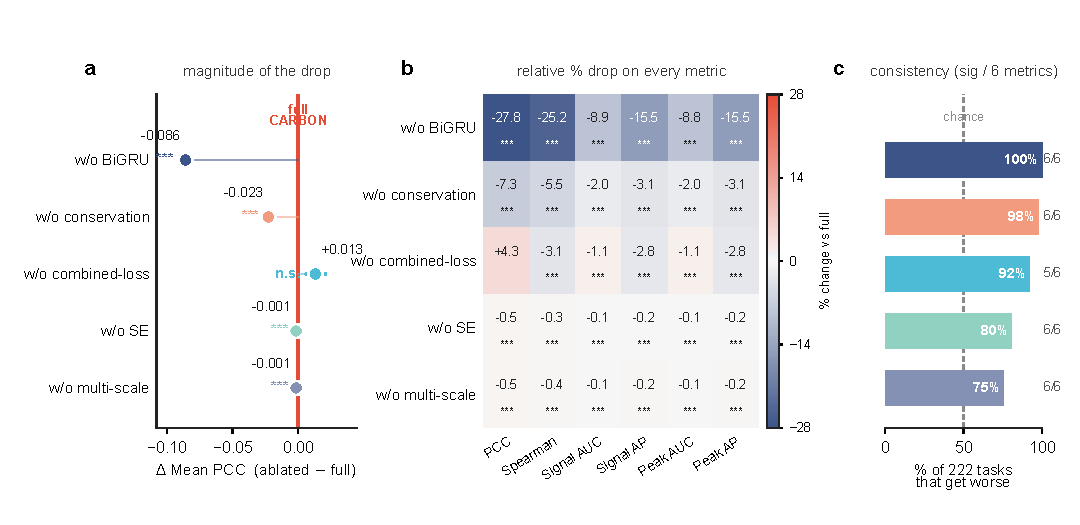
\includegraphics[width=\textwidth]{figS1_ablation.pdf}
\caption{Paired architecture, input and objective ablations over 222 tasks. (a) Signed change in mean pooled task PCC after ablation; positive values indicate improvement. (b) Percentage changes of task means, $100(\bar m_{\rm ablated}-\bar m_{\rm full})/\bar m_{\rm full}$, for each metric; these are not averages of per-task percentage changes. (c) Mean of the six metric-specific percentages of tasks that worsen ($n=222$ per metric), annotated with the number of metrics having uncorrected paired Wilcoxon $p<0.05$; the 50\% line (labelled ``chance'' in the panel) is a visual reference, not a calibrated chance-level null. Stars in a/b denote nominal $p<0.05$ (*), $p<0.01$ (**) and $p<0.001$ (***); n.s. denotes $p\geq0.05$. The reconstruction-loss baseline increases mean PCC while decreasing the other five metrics; its median paired PCC change is negative (S1.4). These descriptive effects do not isolate individual combined-loss terms. Printed tests are nominal, unadjusted for multiple comparisons and do not account for shared RBP identities.}
\label{figsupp:ablation}
\end{figure}

\begin{figure}[H]
\centering
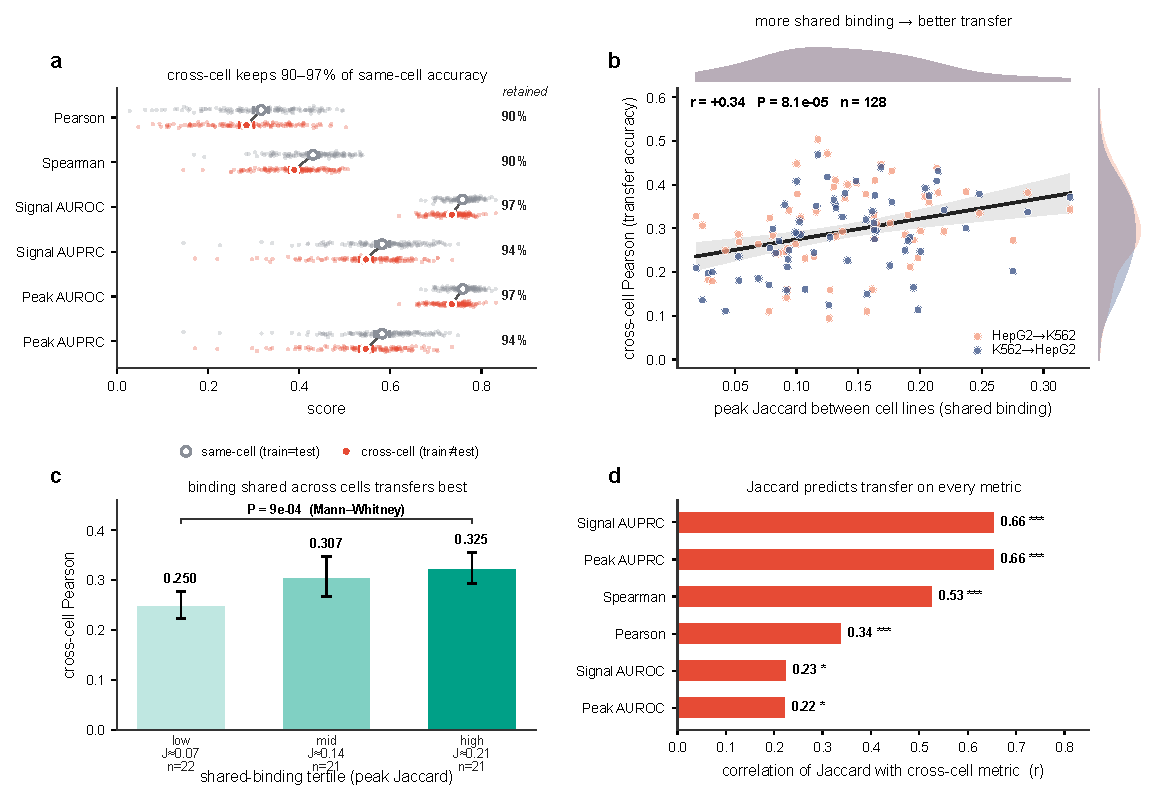
\includegraphics[width=\textwidth]{figS2_crosscell.pdf}
\caption{Cross-cell transfer between HepG2 and K562. (a) Same-cell and cross-cell scores for 70 symbols (140 directional records). Same-cell means the training and evaluation cell lines agree, not that their windows are identical. Large markers and intervals show means $\pm1.96$ standard errors across records; percentages are cross-cell/same-cell mean-score ratios, rather than classification accuracy. AUPRC in the panel denotes the AP metric defined in S1.1. (b) Peak Jaccard overlap versus transferred PCC in the 64-symbol overlap subset (128 directional records), with an OLS fit, nominal 95\% confidence band for its mean response, and marginal densities. (c) Transfer PCC averaged over directions within each of 64 symbols, then grouped by Jaccard tertile ($n=22,21,21$; means 0.250, 0.307 and 0.325). Error bars are $1.96$ standard errors of the symbol means. The nominal one-sided Mann--Whitney test compares high versus low tertiles. (d) Pooled Pearson overlap--score correlations; stars denote nominal $p<0.05$ (*), $p<0.01$ (**) and $p<0.001$ (***). The printed coefficients and nominal $P$ values in b and d use 128 records, with two directions per symbol. Their independence assumption is unmet; the annotations are retained as descriptive summaries and are not evidence from 128 independent symbols.}
\label{figsupp:crosscell}
\end{figure}


\begin{figure}[H]
\centering
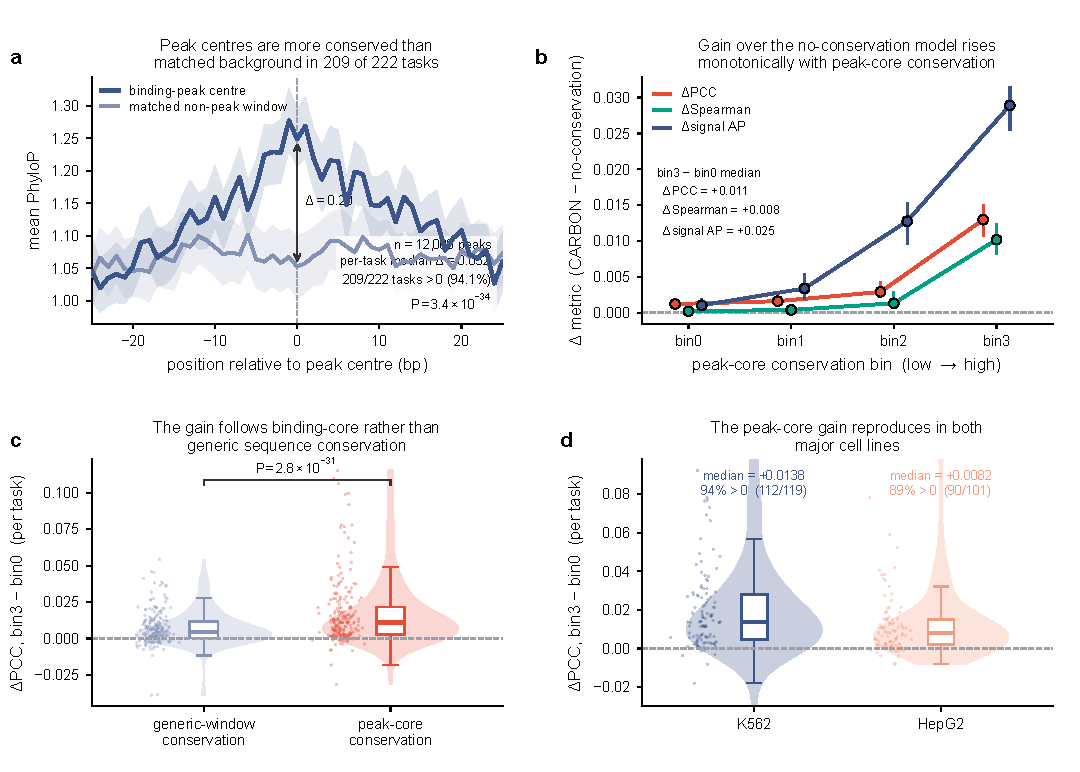
\includegraphics[width=\textwidth]{figS4_conservation_robustness.pdf}
\caption{Complementary conservation summaries. (a) Peak-centred mean PhyloP for 12,000 sampled profiles and non-peak positions within the same windows (the legend's ``matched non-peak window''), with profile-resampling 95\% bootstrap intervals (S1.8). The all-task annotation in a, also plotted in Figure~S12a, is a separate peak/non-peak summary: median task difference 0.0516, positive in 209/222 tasks. (b) Cross-task medians of paired full-minus-no-conservation gains across four peak-core conservation bins, with task-resampling 95\% bootstrap intervals ($n=222$ per bin); annotations give median paired highest-minus-lowest-bin contrasts. (c) Paired endpoint PCC gains under peak-core versus generic-window stratification; peak-core gains are larger in 83.3\% of tasks. (d) Peak-core endpoint PCC gains in K562 (median $+0.0138$, 112/119 positive) and HepG2 (median $+0.0082$, 90/101 positive). In c/d, points represent tasks, violins show their distributions, boxes span the IQR with a median line, and whiskers extend to the most extreme values within 1.5 IQR; separate outlier markers are omitted. The two-sided paired Wilcoxon test in c is nominal and does not account for shared RBP identities. All panels reuse the retained tasks and configuration and are not independent replications.}
\label{figsupp:conservation}
\end{figure}




\begin{figure}[H]
\centering
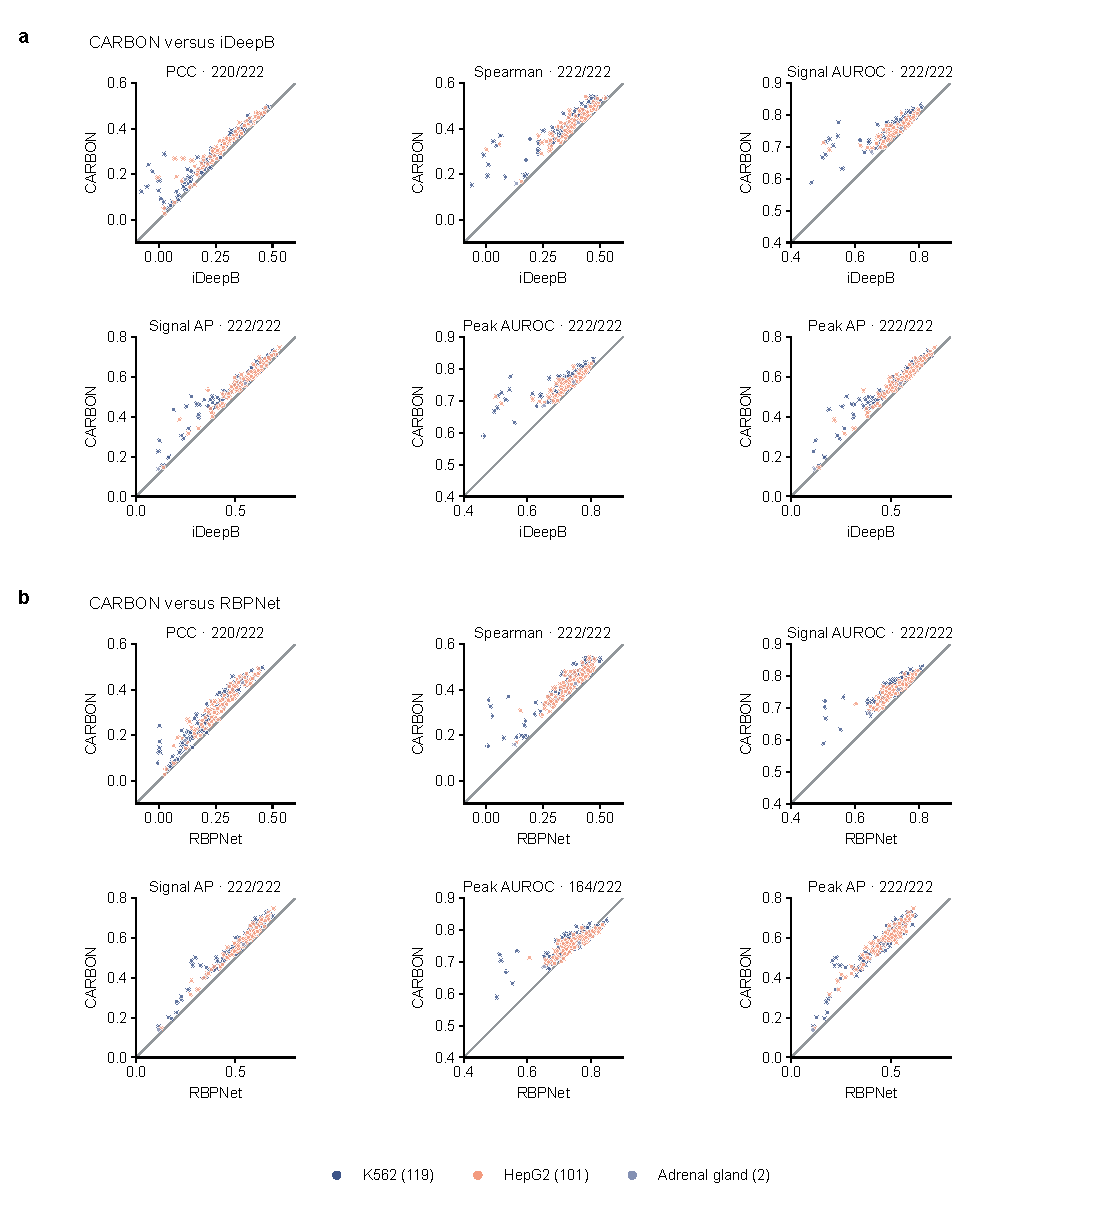
\includegraphics[width=\textwidth]{fig2_supplement_all_metrics.pdf}
\caption{Archived implementation comparison atlas. Output scales and metric implementations are not aligned (S1.3), so the points do not establish a fair method ranking. (a) CARBON versus iDeepB and (b) CARBON versus RBPNet across PCC, Spearman, Signal AUROC, Signal AP, Peak AUROC and Peak AP. Every facet contains all 222 task pairs; its two axes have equal limits and the limits for each metric are identical across comparator rows. The diagonal denotes equality and titles give strict CARBON win counts. K562, HepG2 and adrenal-gland colours match Figure 2. These are task-level endpoint scores; no per-window perturbation endpoint appears here. Source: Data S1/S3.}
\label{figsupp:benchmark_all}
\end{figure}

\begin{figure}[H]
\centering
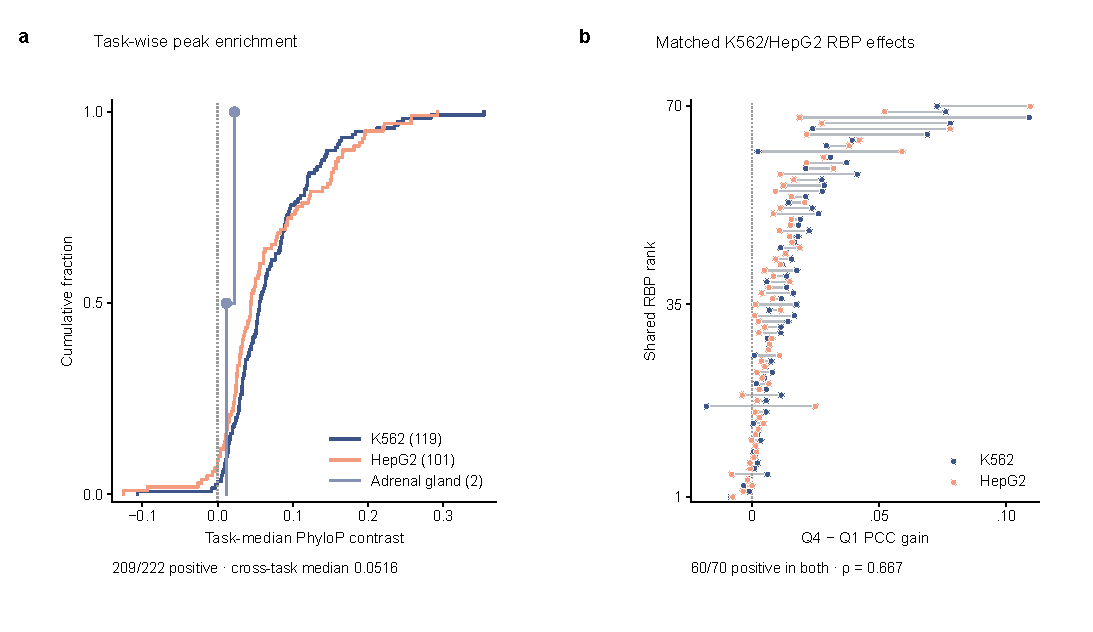
\includegraphics[width=\textwidth]{fig4_supplement_context.pdf}
\caption{Conservation enrichment and shared-RBP context. (a) Empirical distributions of all 222 task-median peak-minus-control PhyloP contrasts by cell/tissue context. (b) Connected K562 and HepG2 Q4-minus-Q1 peak-core PCC gains for all 70 RBPs observed in both contexts, ordered by their pair mean. The cross-context Spearman coefficient is descriptive and the shared genomic/biological structure limits independent-unit interpretation. Sources: Data S7/S8/S12.}
\label{figsupp:conservation_context}
\end{figure}

\begin{figure}[H]
\centering
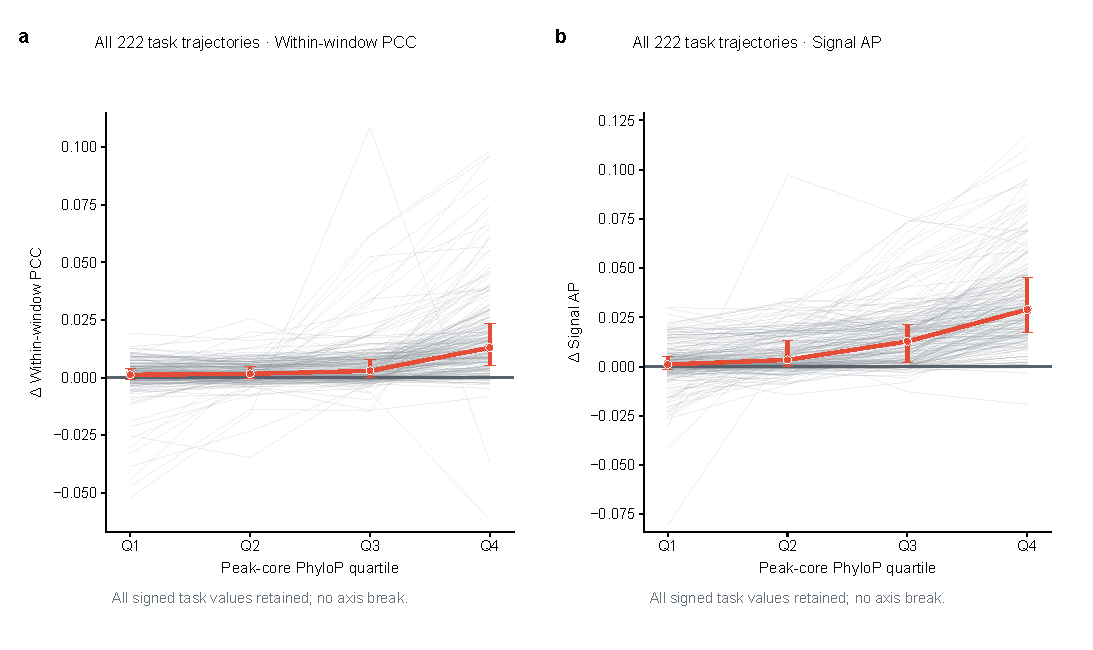
\includegraphics[width=\textwidth]{fig4_supplement_task_trajectories.pdf}
\caption{Complete peak-core conservation quartile task trajectories. (a) Paired within-window PCC gains and (b) Signal AP gains for the same 222 tasks across Q1--Q4. Grey paths retain each task's four linked signed values on an unbroken full-range axis; red markers and intervals denote the cross-task median and IQR, not uncertainty for an RBP-level estimator. Source: Data S8.}
\label{figsupp:conservation_trajectories}
\end{figure}

\begin{figure}[H]
\centering
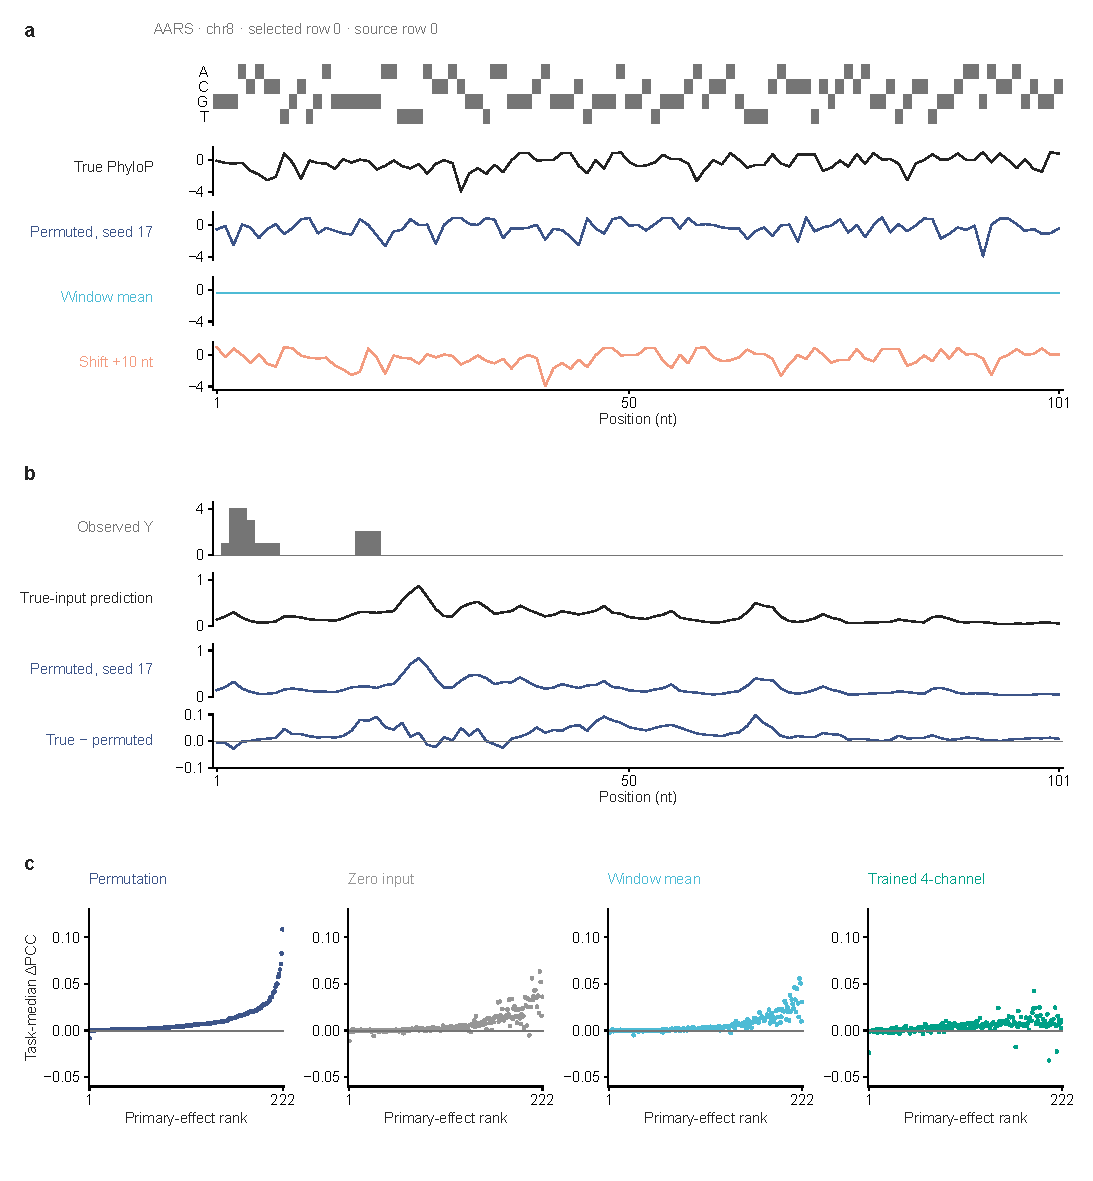
\includegraphics[width=\textwidth]{fig5_supplement_complete_tracks.pdf}
\caption{Complete prespecified perturbation example and task controls. (a) The fixed AARS sequence and aligned true, permuted, window-mean and shifted PhyloP input tracks. (b) Observed signal, true and permuted predictions, and their exact pointwise difference, with separate original signal scales. (c) All 222 signed task-median effects under the primary permutation and three controls in a common ascending primary-effect task order; the separately trained four-channel model is not a zero-input run of the five-channel checkpoint. No task effect is clipped at zero. Sources: Data S11 and the retained AARS example.}
\label{figsupp:perturb_complete}
\end{figure}

\begin{figure}[H]
\centering
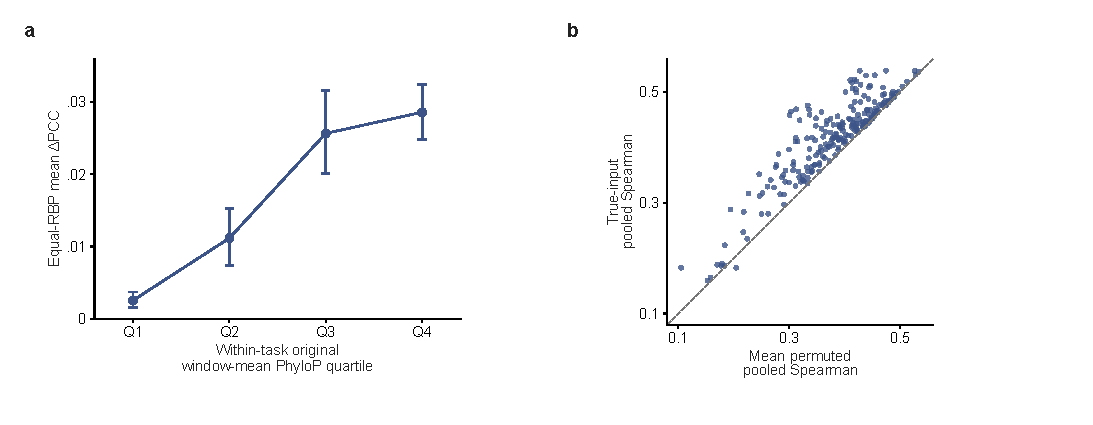
\includegraphics[width=\textwidth]{fig5_supplement_quartile_pooled.pdf}
\caption{Additional frozen-model sensitivity results. (a) Equal-RBP mean primary paired PCC effects by task-specific original whole-window PhyloP quartile Q1--Q4; existing intervals use 5,000 RBP resamples. The Q4-minus-Q1 contrast is 0.02607 (95\% interval 0.02225--0.02988). (b) All 222 true-input pooled Spearman task scores against the arithmetic mean of three separately calculated permutation scores, with equal axes and an identity line; 221 of 222 exceed that mean. Pooled Spearman is distinct from the within-window PCC effect and is not computed from averaged predictions. Sources: Data S11/S13.}
\label{figsupp:perturb_extended}
\end{figure}

\clearpage

\clearpage
\begin{figure}[p]
\centering
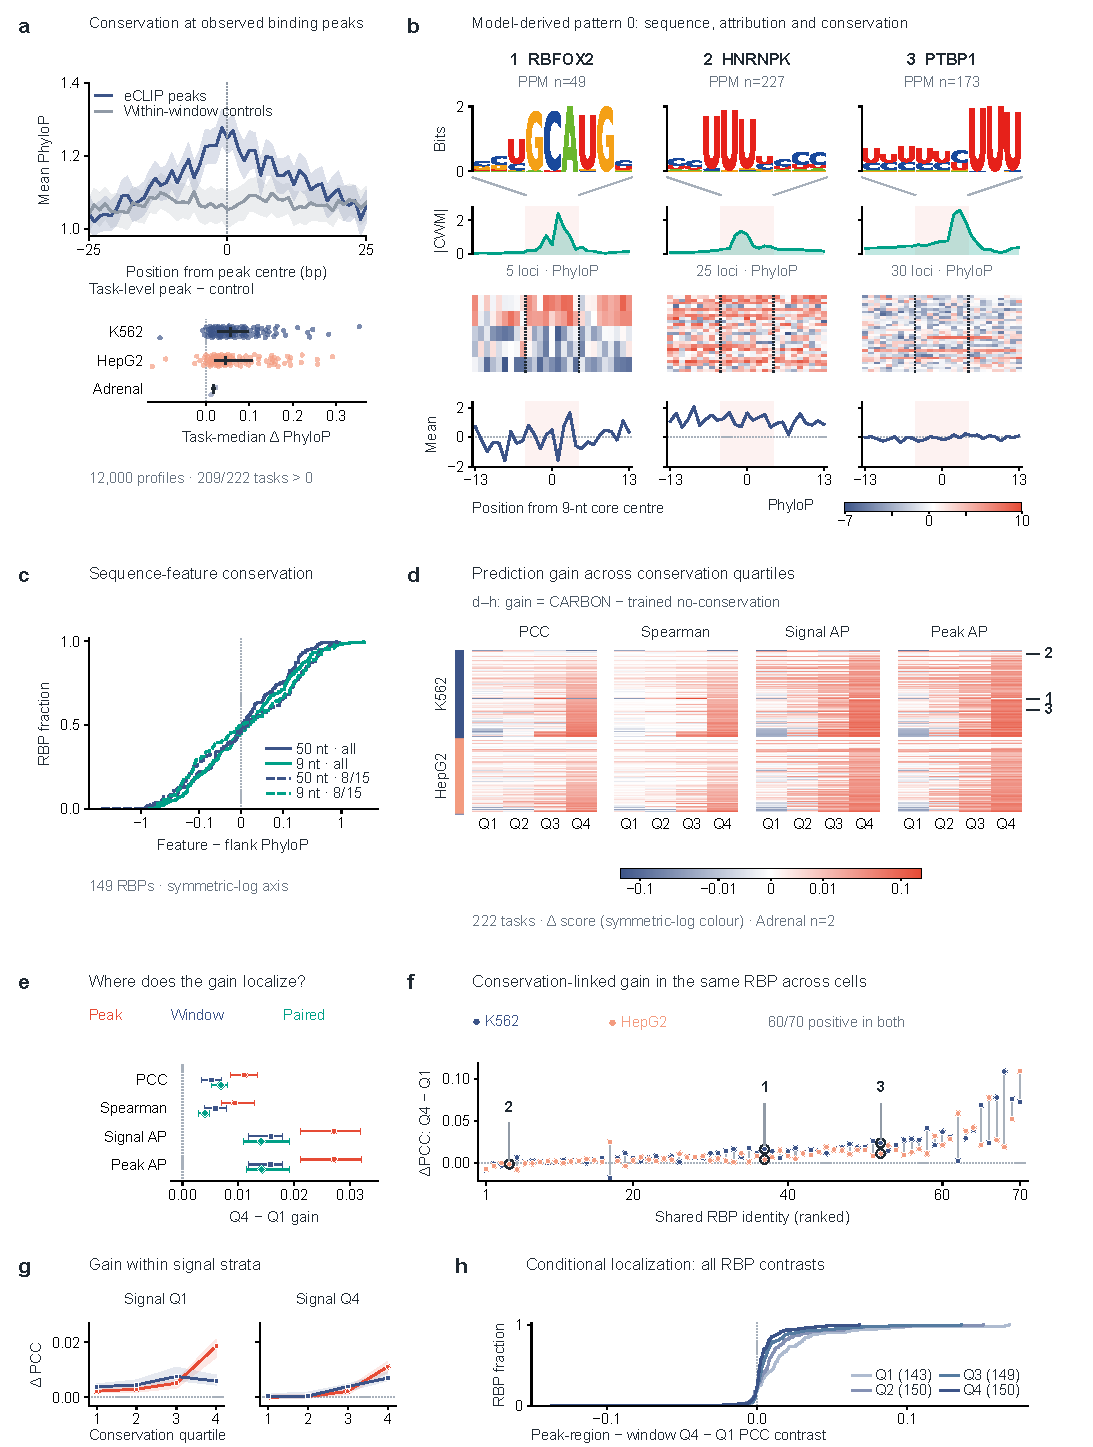
\includegraphics[width=\linewidth,height=.93\textheight,keepaspectratio]{figS9_conservation_complete.pdf}
\caption{Complete conservation evidence. Full panel legend continues on the following page; definitions are in S1.8/S1.12.}
\label{figsupp:extra9}
\end{figure}
\clearpage
{\small\noindent\textbf{Figure S9 legend (continued).} Complete retained conservation evidence. \textbf{a}, The selected 12,000-profile peak/control curves and all task-median peak-minus-control contrasts. \textbf{b}, Fixed RBFOX2/HNRNPK/PTBP1 PPM, contribution and conservation tracks. \textbf{c}, Empirical RBP distributions for original 50-nt segments and distinct 9-nt cores, in the full chromosome-1/8/15 archive and its overlapping chromosome-8/15 subset; both original 50-nt intervals and the 9-nt subset interval contain zero. \textbf{d}, All 3,552 original task--quartile--metric values across PCC, Spearman, Signal AP and Peak AP, with a common task order and complete signed range. \textbf{e}, Peak-region and whole-window Q4-minus-Q1 gains and their paired difference: medians and 95\% bootstrap intervals across 150 RBP summaries. \textbf{f}, All 70 paired K562/HepG2 RBP endpoints; 60 are positive in both contexts. \textbf{g}, Descriptive trained-model PCC-gain curves in the lowest/highest observed-signal strata of the separate 2,079,810-window chromosome-8/15 reanalysis. \textbf{h}, Complete paired localization-contrast distributions for all four signal strata, with 143/150/149/150 available RBPs. Panel g may have different available sets across cells; h performs within-task pairing. Quartiles, populations, estimators and motif limitations are defined in S1.8/S1.12. Identity markers do not assert matched genomic instances; no independent biological replication is implied.\par}

\begin{figure}[H]
\centering
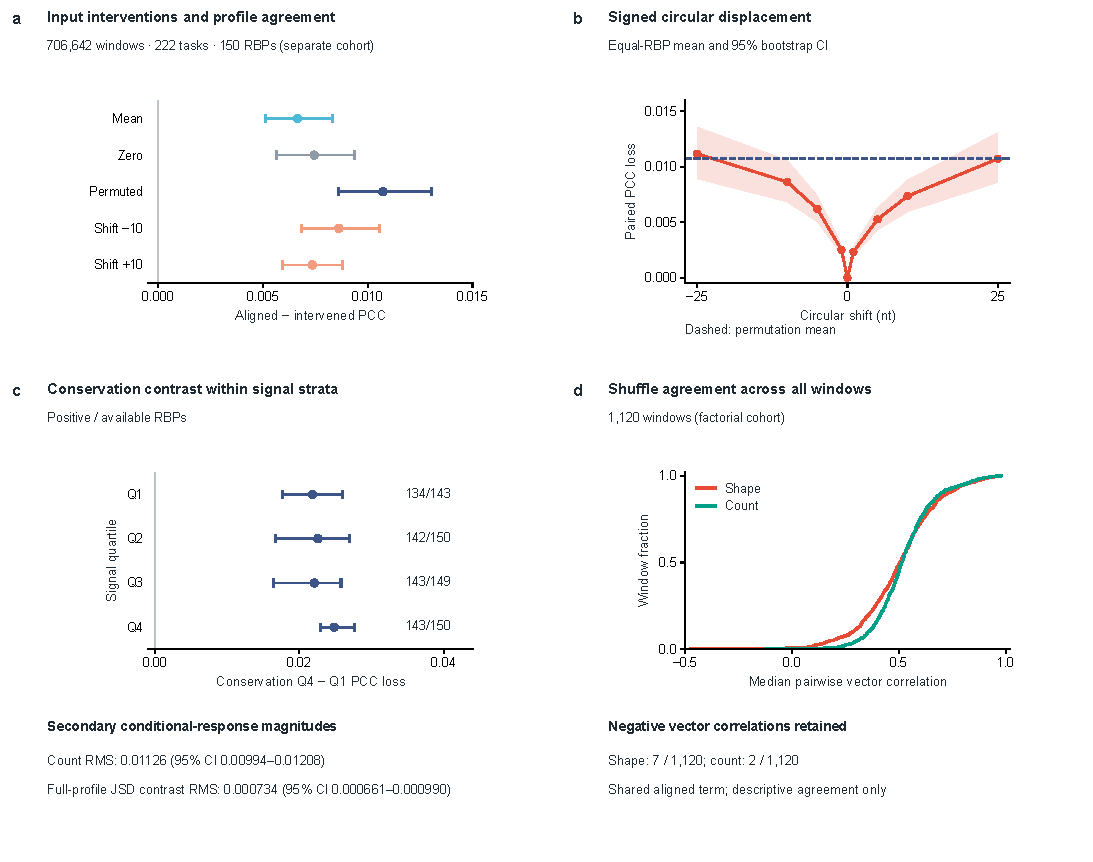
\includegraphics[width=\linewidth]{figS10_perturbation_controls.pdf}
\caption{Bulk controls and secondary sequence-response analyses. \textbf{a,b}, Paired profile-PCC losses in the distinct 706,642-window, 222-task, 150-RBP cohort: task medians, averaged within and then equally across RBPs, with 95\% intervals from 5,000 RBP resamples. Permutation loss subtracts the mean of three separately evaluated correlations; shifts retain the score multiset and mean. Lines connect tested positions only. \textbf{c}, Conservation-Q4-minus-Q1 permutation-loss contrasts within each observed-signal quartile. Signal and conservation quartiles are defined independently within task, then intersected; points show RBP medians and 95\% bootstrap intervals, with positive/available counts. \textbf{d}, All 1,120 factorial-window permutation-agreement summaries, plus secondary count and JSD response summaries. Shape/count agreement vectors share the aligned term and do not constitute independent replication; seven shape and two count correlations are negative and retained. Secondary endpoint aggregation follows S1.13. Bulk and factorial cohorts must not be pooled as independent samples.}
\label{figsupp:extra10}
\end{figure}
\clearpage
\begin{figure}[H]
\centering
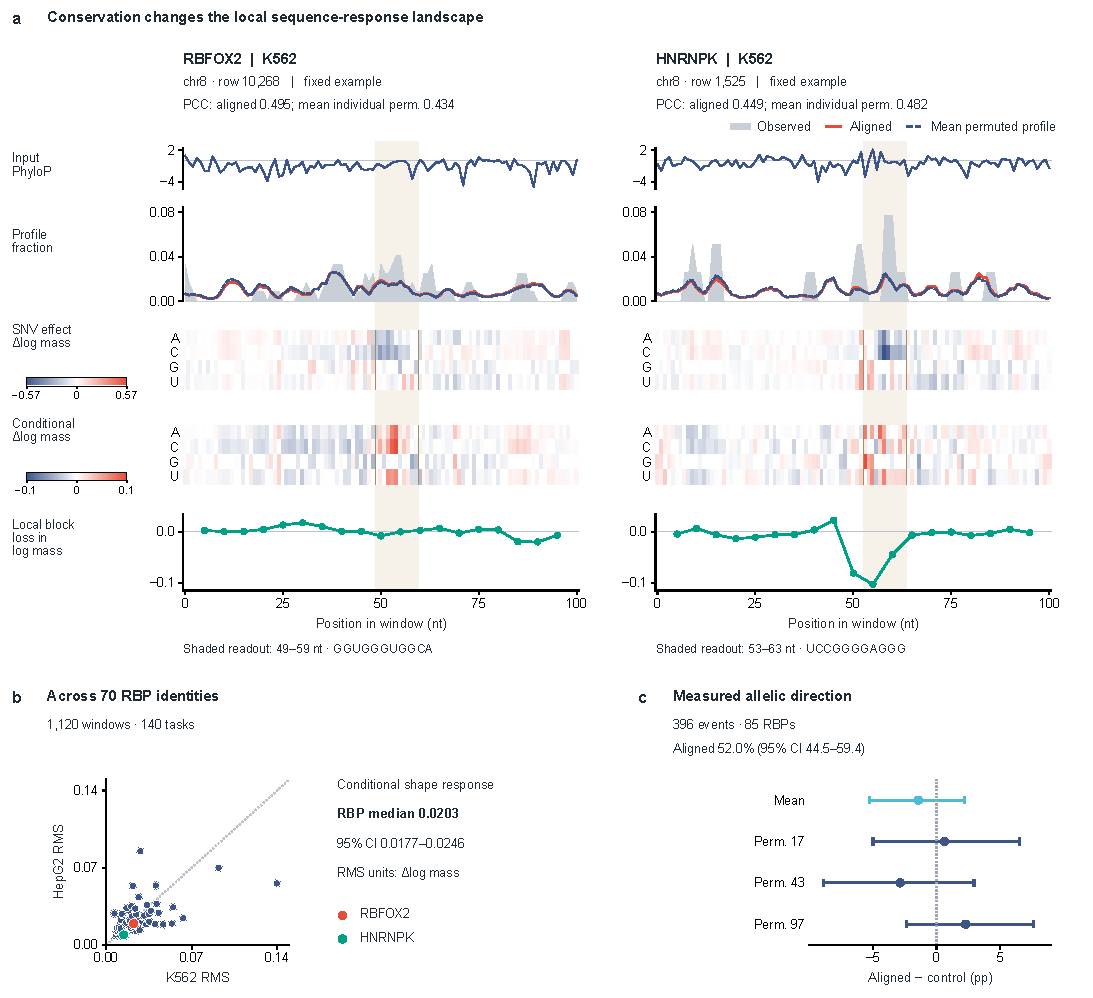
\includegraphics[width=\linewidth]{figS11_sequence_details.pdf}
\caption{Complete local sequence-response views. \textbf{a}, The two fixed K562 windows with actual PhyloP, observed/predicted profiles, absolute aligned-condition substitutions, conditional substitutions and local block responses. Effects use mutant minus same-condition WT log readout mass; conditional effects subtract the mean of three permuted effects. Reference-base cells are blank. Paired cases share signed ranges: absolute substitutions $\pm0.57$, conditional responses $\pm0.10$. Negative block effects are retained. Plotted permutation profiles are averaged, whereas the printed PCC averages individual correlations. \textbf{b}, All 70 shared RBP identities; coordinates are task medians over eight windows, with contexts averaged within RBP before the reported population median. Example labels identify RBP identities, not matched loci. \textbf{c}, The separate positive-ASB direction endpoint from 396 events and 85 RBPs; all paired aligned-minus-control intervals cross zero. Intervals in b,c use 5,000 RBP resamples. These model sensitivities do not establish improved mutant prediction or biological epistasis (S1.13--S1.14).}
\label{figsupp:extra11}
\end{figure}

\clearpage
\begin{figure}[p]\centering
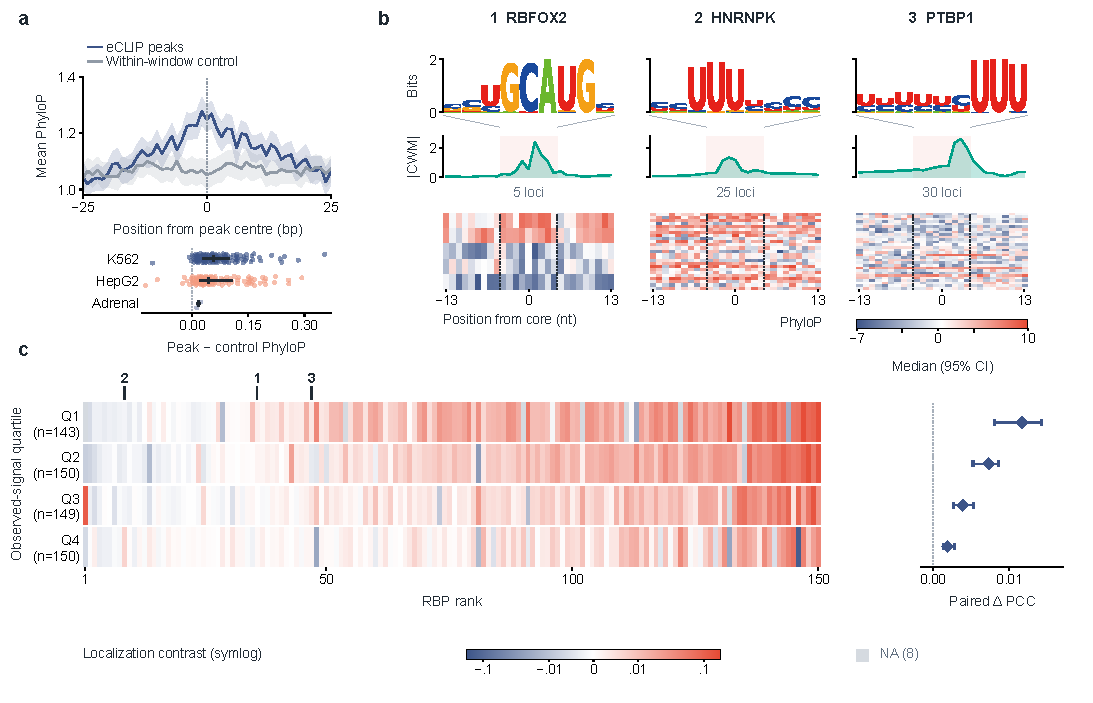
\includegraphics[width=.93\linewidth]{figS12_previous.pdf}
\caption{Conservation localization across binding sites and signal contexts. \textbf{a}, Mean PhyloP for 12,000 selected peak-centred profiles and within-window controls, with separate 95\% profile-bootstrap bands (300 resamples); below, all 222 task-median peak-minus-control contrasts. \textbf{b}, Fixed K562 pattern-0 examples RBFOX2, HNRNPK and PTBP1 (1--3): 9-nt PPM logos, aligned 27-nt absolute contribution weights, every retained conservation locus, and position-wise means. PPMs contain 49/227/173 discovery seqlets; conservation tracks contain 5/25/30 loci. \textbf{c}, All available RBP localization contrasts across observed-signal quartiles: peak-region conservation Q4-minus-Q1 PCC gain minus its whole-window counterpart. Gain is CARBON minus the trained no-conservation model; pairing precedes within-RBP averaging. All 592 finite cells are retained; eight unavailable cells are grey. Diamonds show row medians and 95\% RBP bootstrap intervals. Labels 1--3 link RBP identities, not genomic windows. The map uses 2,079,810 eligible chromosome-8/15 records. Symmetric-log colours retain signed values without saturation; linear thresholds are $\pm1$ PhyloP in b and $\pm0.01$ PCC in c. Population motif checks and full endpoint analyses are in Supplementary Fig.~S9; definitions and scope in S1.12. These associations do not establish causal or universal motif conservation.}
\label{figsupp:previous4}\end{figure}

\clearpage
\begin{figure}[p]\centering
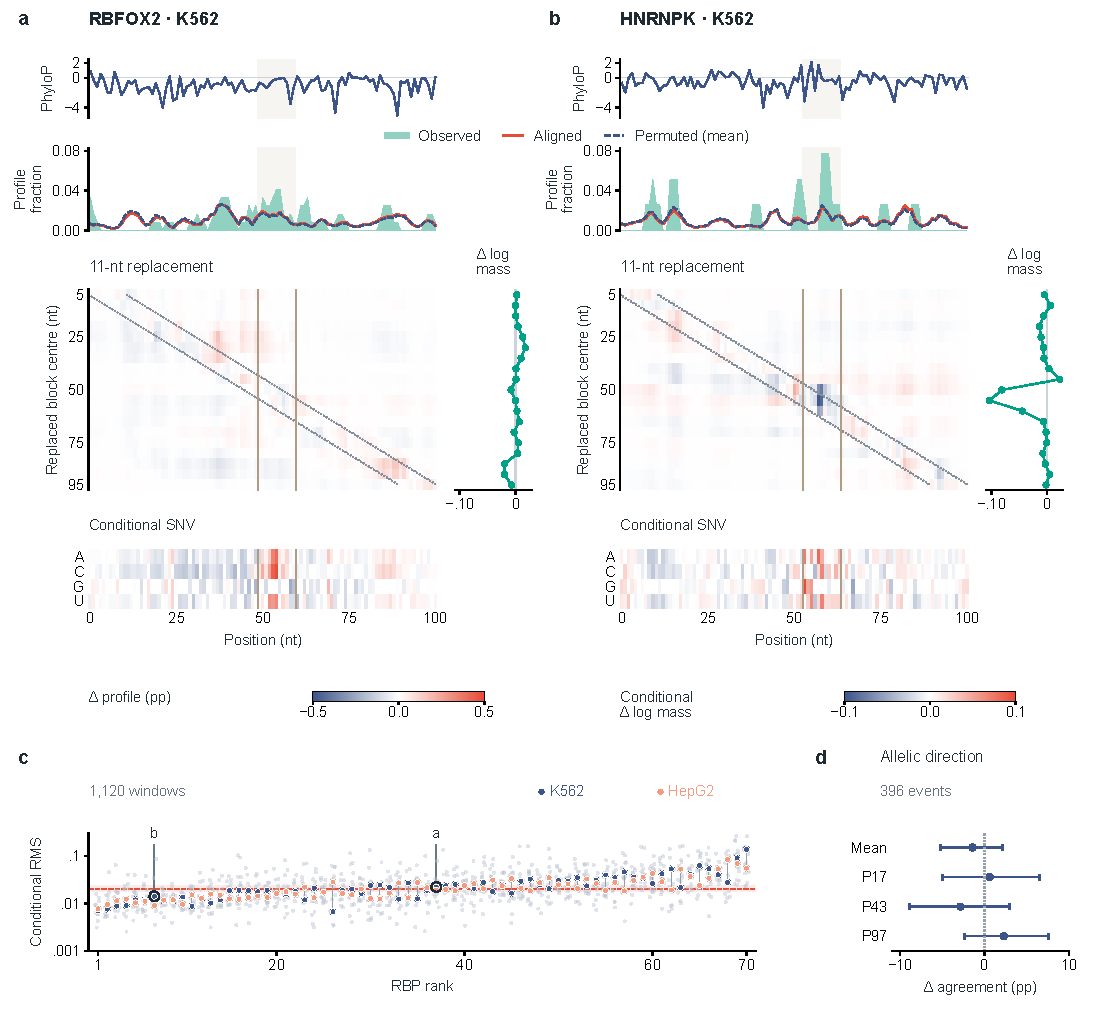
\includegraphics[width=.93\linewidth]{figS13_previous.pdf}
\caption{Spatial conservation dependence of modelled sequence responses. \textbf{a,b}, Protocol-fixed RBFOX2 and HNRNPK K562 windows. Tracks share the 101-nt coordinate; shaded readouts span positions 49--59 and 53--63 (zero-based). Aligned versus mean individual permutation PCC is 0.495 versus 0.434 (RBFOX2) and 0.449 versus 0.482 (HNRNPK); the plotted permutation profile is the mean of three predictions. Each map row replaces an 11-nt conservation block by the window mean. Colours show aligned-minus-replaced output probability in percentage points; teal margins show the same-direction log-readout-mass difference. Negative effects remain. Conditional SNV strips show all 303 mutant-minus-WT responses under aligned conservation minus the permutation-mean response, with condition-specific WT and blank reference cells. \textbf{c}, All 1,120 windows and 140 task medians from 70 shared RBPs. Links pair contexts by protein identity; rank orders their mean task medians. The dashed median and band use 5,000 RBP bootstrap resamples; RMS measures magnitude, not accuracy. \textbf{d}, Aligned-minus-control allelic-direction agreement for 396 published ASB events (85 RBPs), with paired 95\% RBP intervals. All intervals cross zero. The positive-ASB-only, ENCODE-family cohort is not independent biological validation. Supplementary Figs.~S10--S11 retain controls and secondary readouts; S1.13--S1.14 define the distinct cohorts, scales and estimators.}
\label{figsupp:previous5}\end{figure}

\clearpage
\begin{figure}[p]\centering
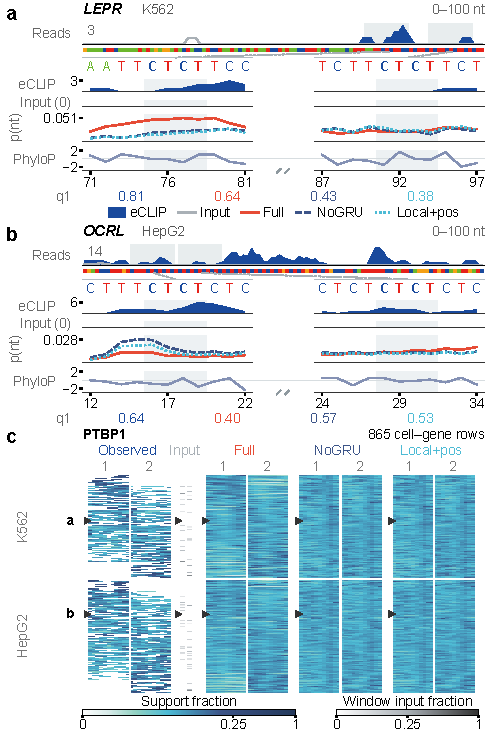
\includegraphics[width=85mm]{figS14_previous_LEPR.pdf}
\caption{LEPR illustration and complete native allocation atlas. LEPR (K562) and OCRL (HepG2) connect 101-nt native signal and sequence to two 11-nt supports. Identity glyphs are not attribution; the coordinates omit the native gap. LEPR was a post hoc example fixed before Local+pos predictions. Its atlas row averages five pairs, whereas the detail shows one member; OCRL has one pair. All 1,851 PTBP1 pairs/865 cell--gene rows remain with the same observed-share order. Detail probabilities retain native 101-nt normalization; the atlas jointly conditions raw counts and mean profiles on the two supports per pair. Input stripes separately show whole-window-input fractions. Statistics and transformation definitions are unchanged from S1.17. LEPR complements the selected ZMYM4 illustration within the same allocation population.}
\label{figsupp:previous_lepr}\end{figure}

\clearpage
\begin{figure}[p]\centering
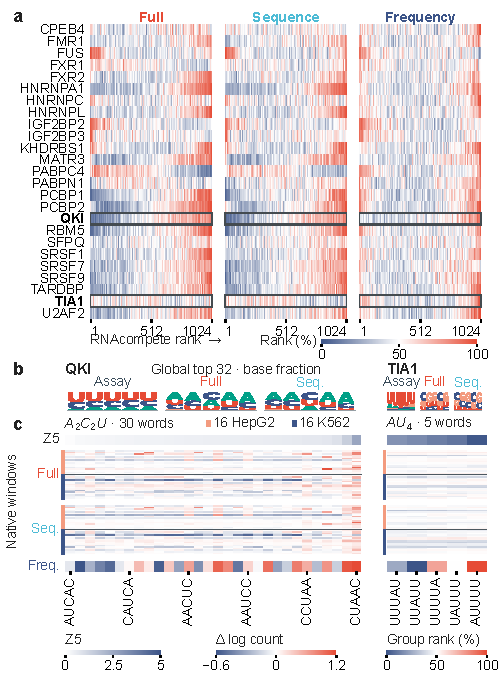
\includegraphics[width=85mm]{figS15_word_landscape.pdf}
\caption{Complete sequence-preference landscapes and retained weak TIA1 example. \textbf{a}, All 25 proteins, with 1,024 words ordered independently by mean external preference per protein. Each plotted column averages eight neighboring words, retaining all words; the rank of a pooled mean response is a descriptive display and differs from the frozen task/assay metric. \textbf{b}, Positional base fractions among the global top 32 words for external preference, Full and Sequence. These identity summaries are not attribution or validated motifs. \textbf{c}, Every word in QKI's externally selected A$_2$C$_2$U group (30) and TIA1's AU$_4$ group (five), in external order, with all 16 HepG2 and 16 K562 model-response contexts. Frequency uses within-group average-tie ranks. RNAcompete $Z_5$ is an occurrence-weighted seven-mer proxy, not a direct five-mer affinity assay. Full has no general advantage over Sequence. The weak TIA1 order response and all adverse contexts remain. Definitions and complete endpoints are in S1.18/Data S23.}
\label{figsupp:word_landscape}\end{figure}

\clearpage
\begin{figure}[p]\centering
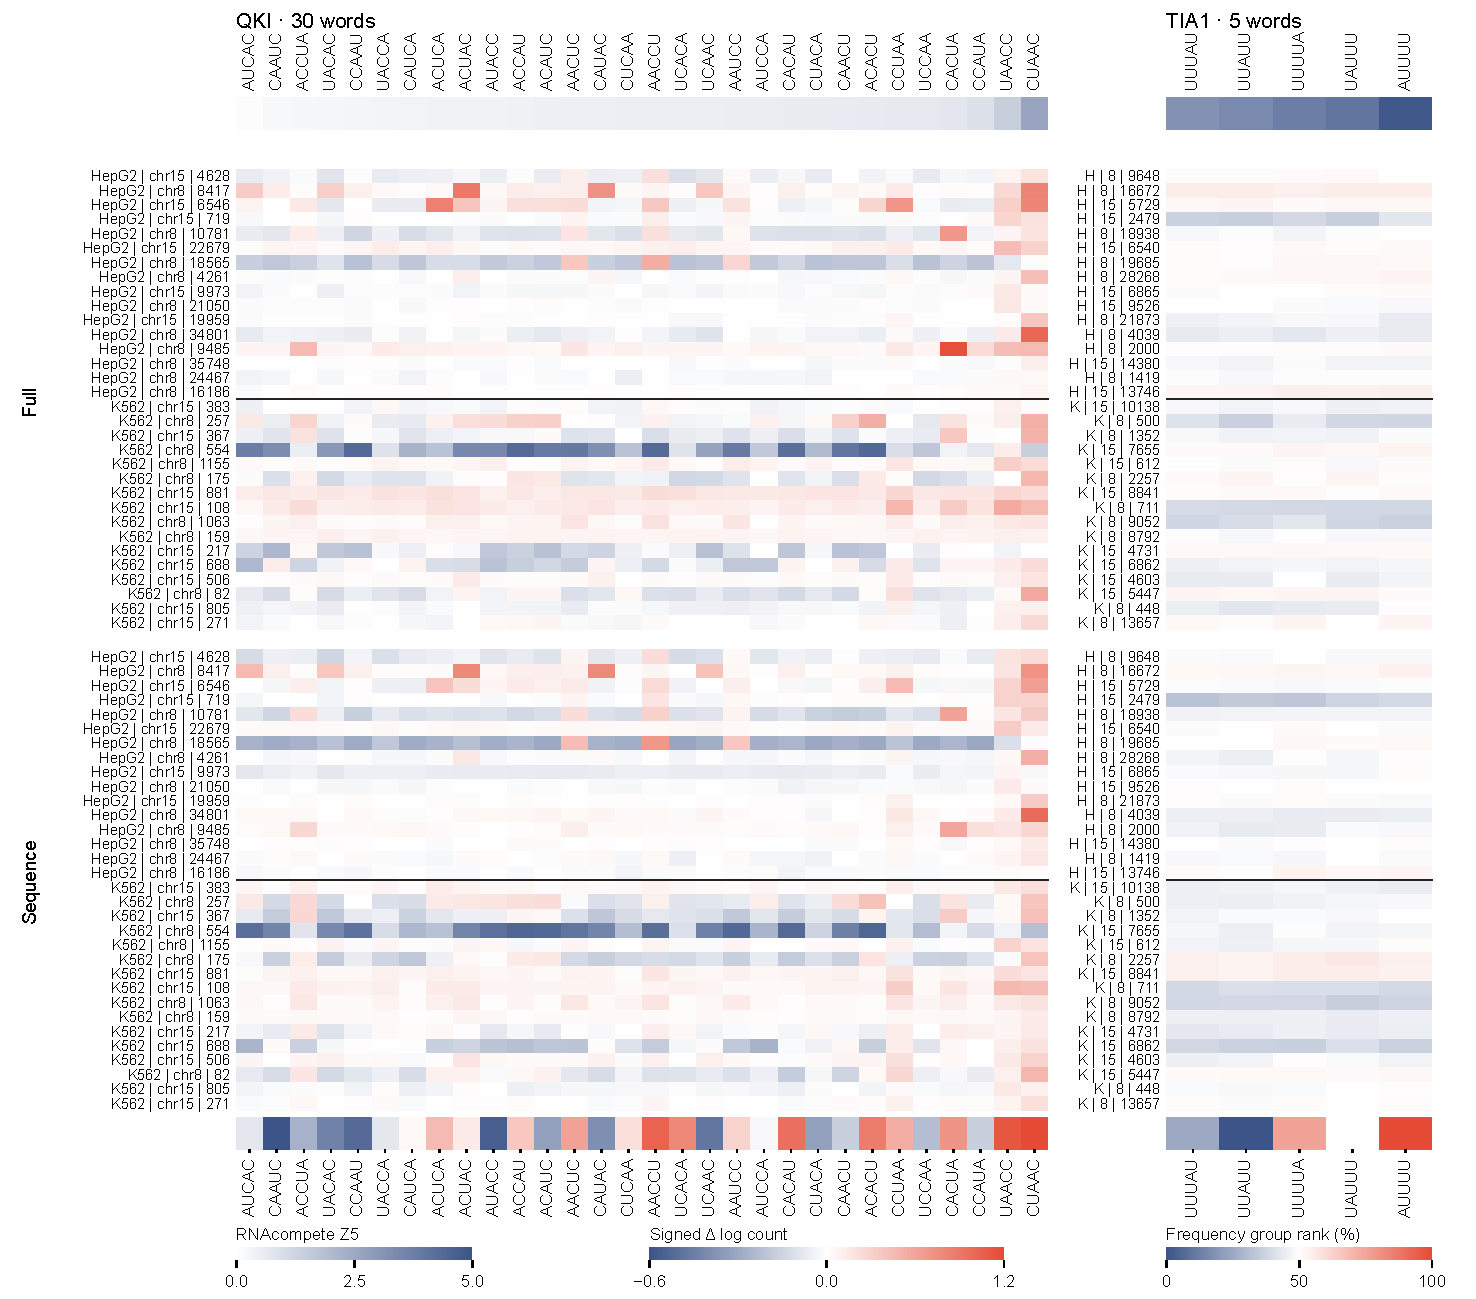
\includegraphics[width=\linewidth,height=.79\textheight,keepaspectratio]{figS16_composition_detail.pdf}
\caption{Enlarged complete QKI/TIA1 composition landscapes. Every word in the externally selected 30-word QKI and five-word TIA1 groups is shown with independent $Z_5$, signed Full/Sequence outputs in all 32 native backgrounds and native Frequency. The display preserves unfavorable and weak responses, without changing the frozen primary or secondary endpoints. Its sequence-group selection, transformations and units are defined in S1.18.}
\label{figsupp:composition_detail}\end{figure}

\clearpage
\begin{figure}[p]\centering
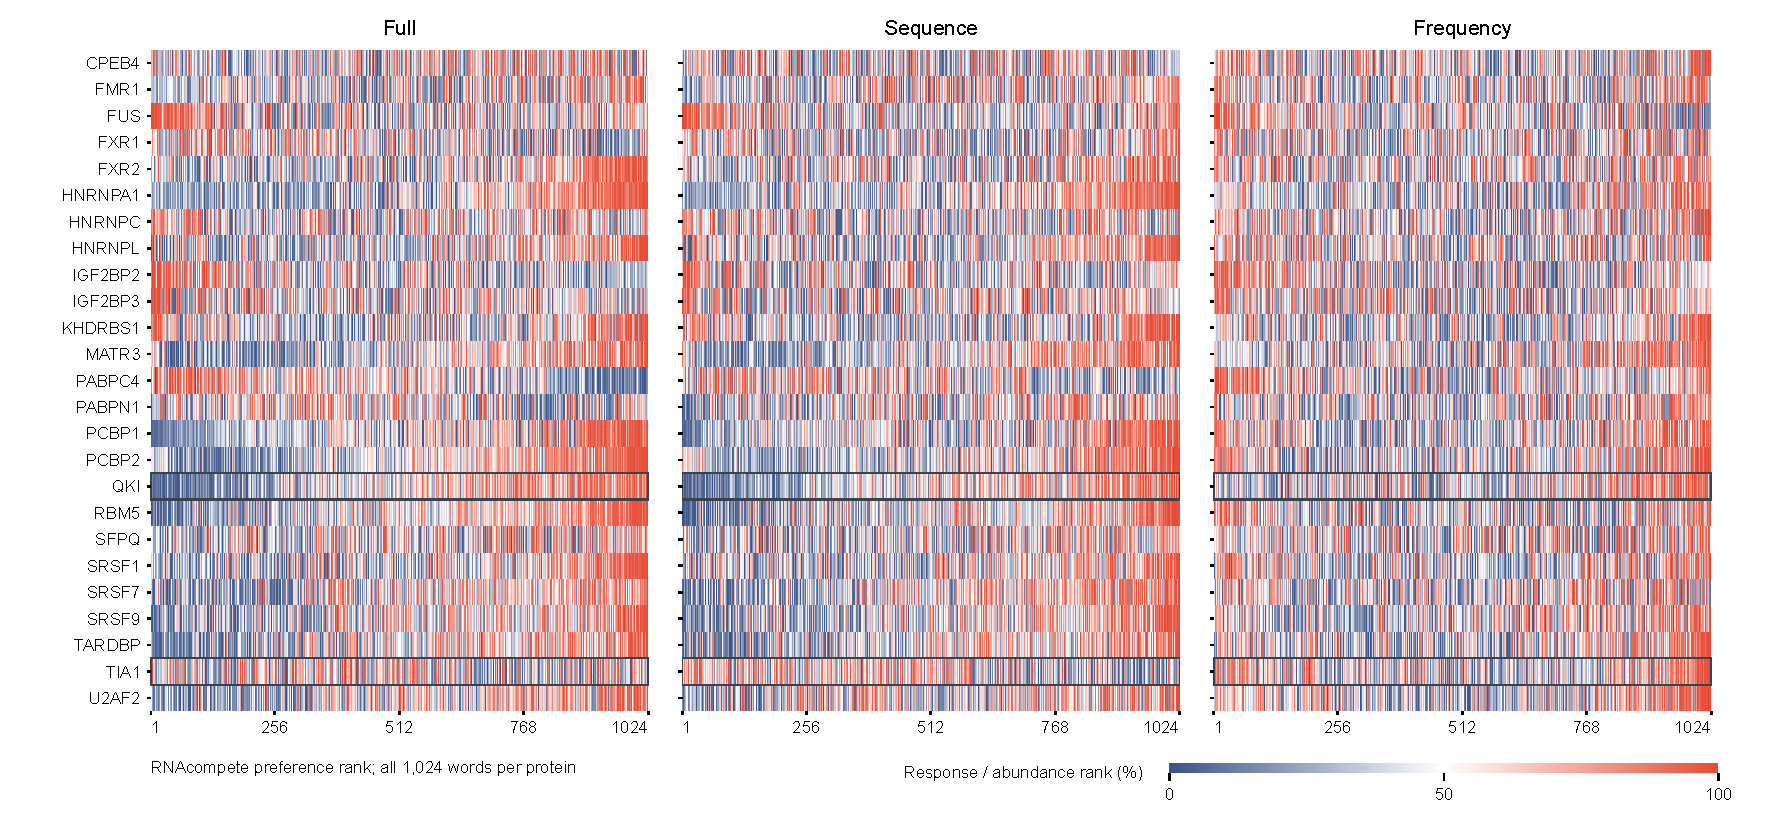
\includegraphics[width=\linewidth,height=.79\textheight,keepaspectratio]{figS17_full_word_atlas.pdf}
\caption{Enlarged all-1,024-word descriptive atlas for all 25 proteins. Each protein orders columns by its own mean external preference. Full/Sequence word-response ranks and native Frequency retain the entire vocabulary. Protein-wise display pooling is distinct from the original task/assay correlation and concordance calculations. Data S23 supplies exact values; S1.18 defines the frozen inference and aggregation.}
\label{figsupp:full_word_atlas}\end{figure}

\clearpage
\begin{figure}[p]\centering
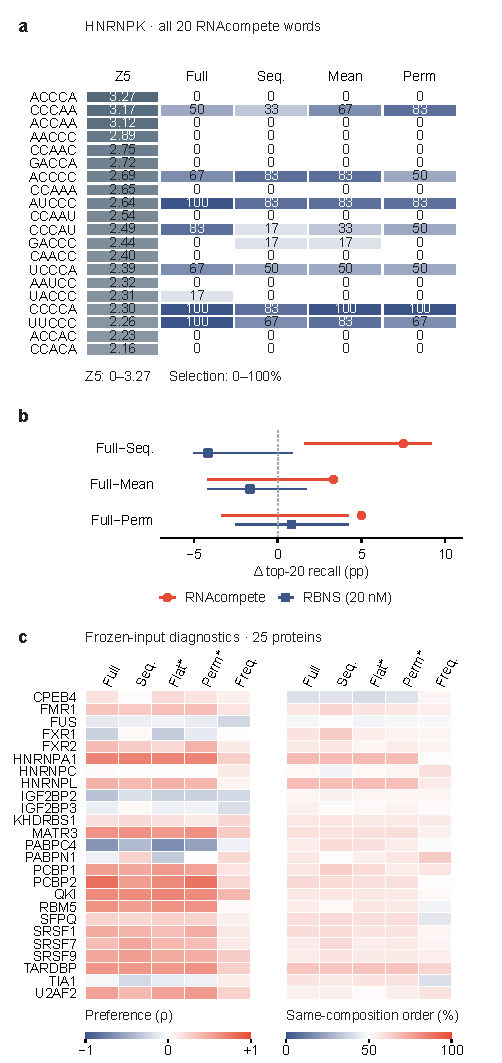
\includegraphics[width=\linewidth,height=.79\textheight,keepaspectratio]{figS18_preference_controls.pdf}
\caption{External-preference controls and assay-specific limits. All 25 protein-level frozen-input conservation controls, complete exposed HNRNPK word-priority diagnostics and trained controls are retained. The favorable RNAcompete diagnostic and unfavorable preselected 20-nM RBNS result concern the previously exposed protein and do not enter the new 25-protein validation summary. The source-specific endpoints, units and limitations are given in S1.18 and Data S23.}
\label{figsupp:preference_controls}\end{figure}


\clearpage
\begin{figure}[p]\centering
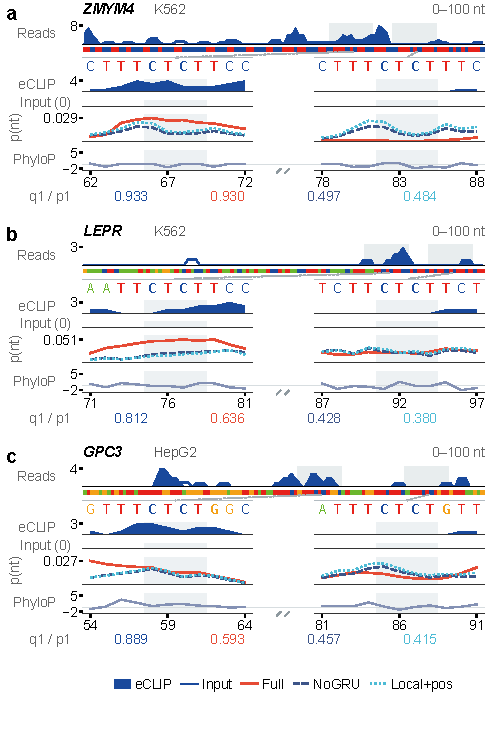
\includegraphics[page=1,width=120mm]{figS19_context_examples.pdf}
\caption{Complete post hoc candidate set and retained failure, first three cases. Native 101-nt eCLIP/input context, nucleotide identity, enlarged supports, three-seed mean profiles, PhyloP and support shares follow Figure~4a,b. The complete set contains eight qualifying cases, in frozen rank order, followed by the retained OCRL failure. They illustrate the post hoc rule, not an independent success rate. The selection funnel is $1,851\to86\to55\to42\to33\to8$: identical seven-mers, $|q_1-0.5|\geq0.2$, at least ten support counts, correct Full direction and incorrect directions for both controls. Exact predicted ties are excluded; ranking uses the smaller control-minus-Full squared-error improvement, then pair hash. Definitions and all selection flags are in S1.17/Data S22.}
\label{figsupp:allocation_examples}
\end{figure}
\clearpage
\begin{figure}[p]\ContinuedFloat\centering
\includegraphics[page=2,width=120mm]{figS19_context_examples.pdf}
\caption{Complete post hoc candidate set, continued. STAG2, ALG13 and SMYD3 are the fourth through sixth candidates under the same frozen rule. Count and probability scales are shown per case; the PhyloP axes share $[-3,6]$ across all nine cases and Figure~4a,b, retaining every value. Probability tracks retain whole-window normalization. $q_1$ is the input-adjusted observed share and $p_1$ the model share for support~1.}
\end{figure}
\clearpage
\begin{figure}[p]\ContinuedFloat\centering
\includegraphics[page=3,width=120mm]{figS19_context_examples.pdf}
\caption{Complete post hoc candidate set and retained failure, continued. RABGAP1L and TAL1 complete the eight qualifying cases; OCRL is the previously retained failure, not selected by a new failure-ranking rule. Native support slices, source identities, profiles and shares accompany Data S22. These examples use existing predictions without model retraining.}
\end{figure}
\clearpage
\begin{figure}[p]\centering
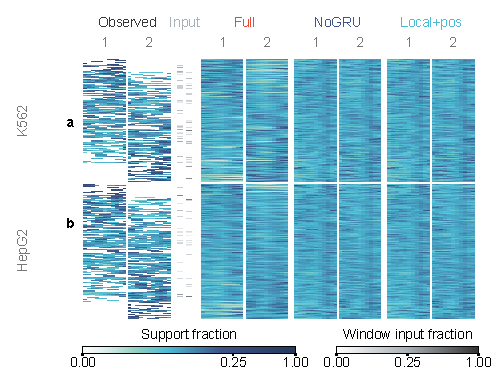
\includegraphics[width=150mm]{figS20_raw_allocation_atlas.pdf}
\caption{Complete raw support-conditioned allocation atlas. All 1,851 eligible pairs, 659 genes and 865 cell--gene rows retain their frozen adjusted-observed-share order. Observed counts and three-seed mean Full, NoGRU and Local+pos profiles are conditioned jointly over both 11-nt supports before equal-pair gene averaging. The common support-fraction scale is 0--1 with power $\gamma=0.25$. Input stripes separately show support fractions of whole-window input, with $\gamma=0.5$; their row sums can be below one. All 1,565 zero-local-input pairs remain zero. Numbers 1/2 identify supports; rules separate K562 and HepG2. Labels a/b link to Figure~4a,b; ZMYM4's row averages two pairs and OCRL's one. Arrays, normalization and ordering are unchanged; main Figure~4c shows the same matrices with the common map and paired raw-share strips and cell-wise observed-versus-Full scatterplots defined in S1.17.}
\label{figsupp:raw_allocation_atlas}\end{figure}
\clearpage
\begin{figure}[p]\ContinuedFloat\centering
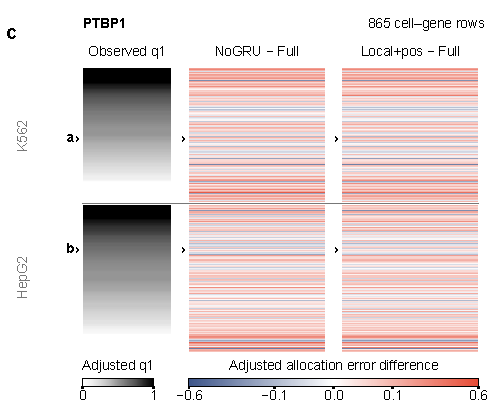
\includegraphics[width=150mm]{figS20_adjusted_error_atlas.pdf}
\caption{Complete input-adjusted allocation-error atlas. The same 865 cell--gene rows retain all 1,851 pairs and frozen ordering. Grey gives mean adjusted observed $q_1$; columns give equal-pair mean squared-error differences, NoGRU minus Full and Local+pos minus Full. Red indicates smaller Full error, blue larger Full error and zero is white. Both columns retain the common symmetric signed-square-root map over $[-0.6,0.6]$, with ticks in original error units and no clipping. Rules separate cells; a/b identify native-example rows. These adjusted errors are distinct from the raw support-conditioned profiles in main Figure~4c. The primary equal-gene/equal-cell estimate and frozen bootstrap intervals are unchanged.}
\end{figure}


\clearpage
\begin{figure}[p]\centering
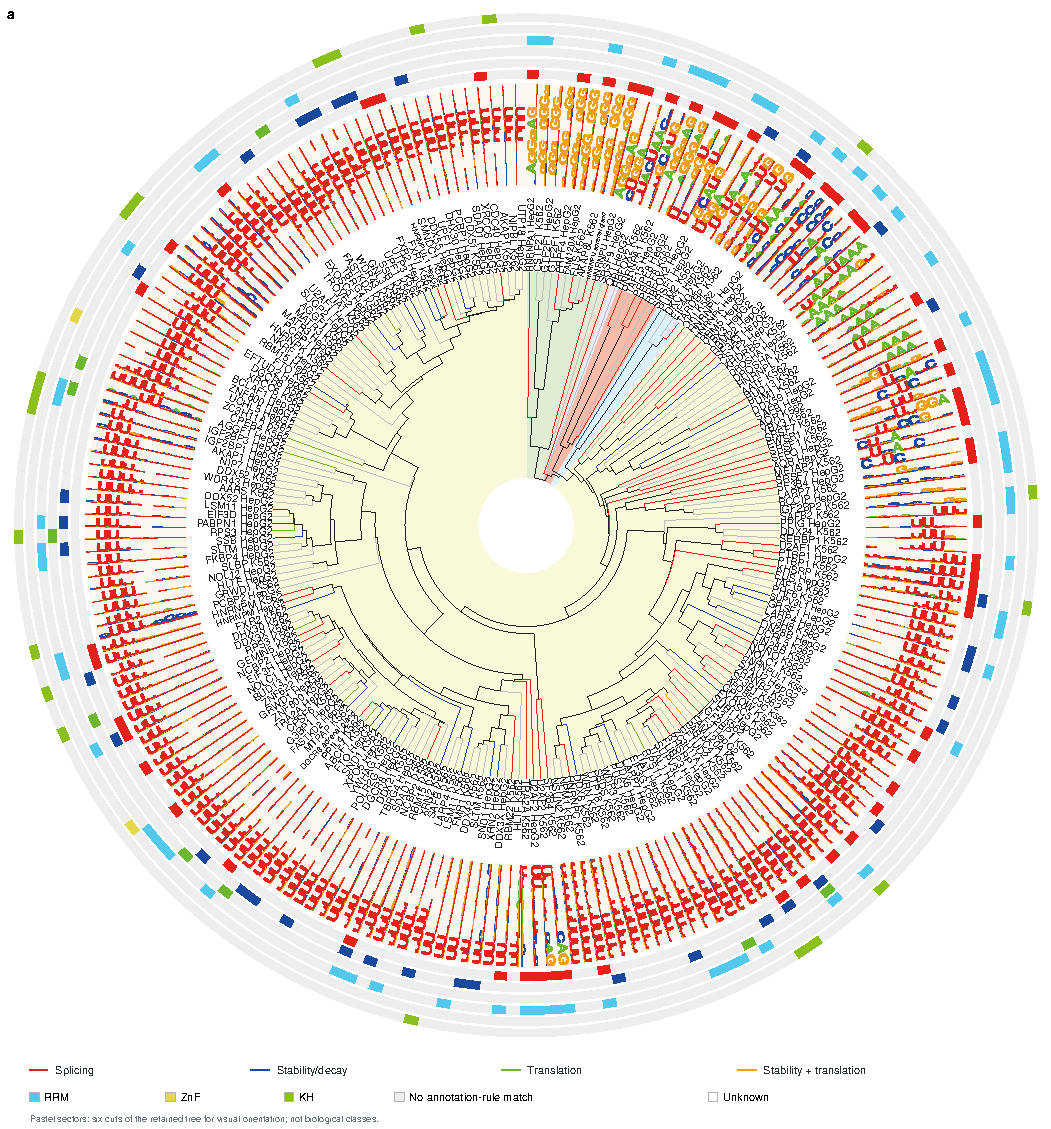
\includegraphics[page=1,width=\linewidth]{figS21_motif_atlas.pdf}
\caption{Full-name motif atlas supporting Figure~3a. All 219 positive pattern-0 entries, frozen leaf order, maximal-information 9-nt crops and six annotation tracks are preserved. The overview is followed by enlarged quadrant views for readable names. Inner-to-outer rings indicate splicing, stability/decay, translation, RRM, ZnF and KH. Clustering uses Euclidean distance between row-normalized PPM crops and average linkage. The adapted R/circlize rendering adds six pastel cuts of this same tree for orientation only; these sectors do not identify six biological classes. No structural-preference information is inferred. This similarity overview does not imply significant experimental-reference matching for every leaf. Data S10 supplies leaf identities; Data S24 preserves all reference comparisons and source classes.}
\label{figsupp:motif_atlas}\end{figure}
\clearpage
\begin{figure}[p]\ContinuedFloat\centering
\includegraphics[page=2,width=\linewidth]{figS21_motif_atlas.pdf}
\caption{Full-name motif atlas, upper-left quadrant. Definitions and the complete source mapping follow the overview.}
\end{figure}
\clearpage
\begin{figure}[p]\ContinuedFloat\centering
\includegraphics[page=3,width=\linewidth]{figS21_motif_atlas.pdf}
\caption{Full-name motif atlas, upper-right quadrant. Annotation tracks and motif matrices are unchanged.}
\end{figure}
\clearpage
\begin{figure}[p]\ContinuedFloat\centering
\includegraphics[page=4,width=\linewidth]{figS21_motif_atlas.pdf}
\caption{Full-name motif atlas, lower-left quadrant. Shared quadrant boundaries do not introduce additional observations.}
\end{figure}
\clearpage
\begin{figure}[p]\ContinuedFloat\centering
\includegraphics[page=5,width=\linewidth]{figS21_motif_atlas.pdf}
\caption{Full-name motif atlas, lower-right quadrant. The source table retains every full task identifier.}
\end{figure}

\clearpage
\begin{figure}[p]\centering
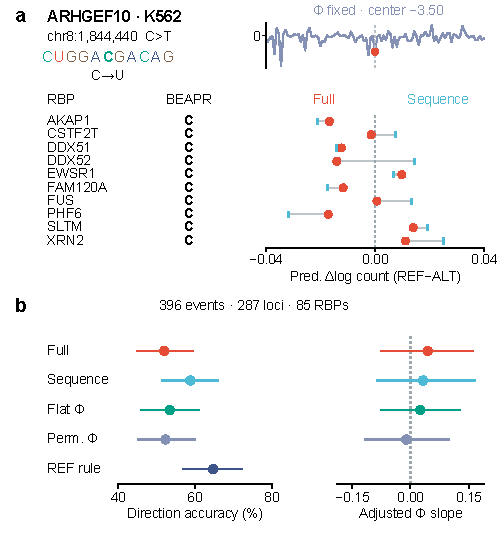
\includegraphics[width=150mm]{figS22_natural_snv.pdf}
\caption{Natural-SNV illustration and complete chromosome-subset analysis. \textbf{a}, All ten K562 RBP events at chr8:1,844,440 C$>$T, selected by maximal RBP coverage. Allele sequences differ only at the central base; both receive the same unchanged reference PhyloP. BEAPR entries identify preferred alleles; positive predicted change denotes REF$>$ALT. Full and Sequence recover four and six directions. \textbf{b}, All 396 chromosome-8/15 events: RBP-equal direction accuracy (left, 5,000 RBP bootstrap draws) and conservation-associated directional-credit slopes (right, approximate two-way RNA-region/RBP multiplier intervals). REF, flat and permuted controls remain. This exposed, ASB-positive cohort cannot validate ASB detection or pathogenicity. See S1.20/Data S25.}
\label{figsupp:natural_snv}\end{figure}
\clearpage
\begin{figure}[p]\centering
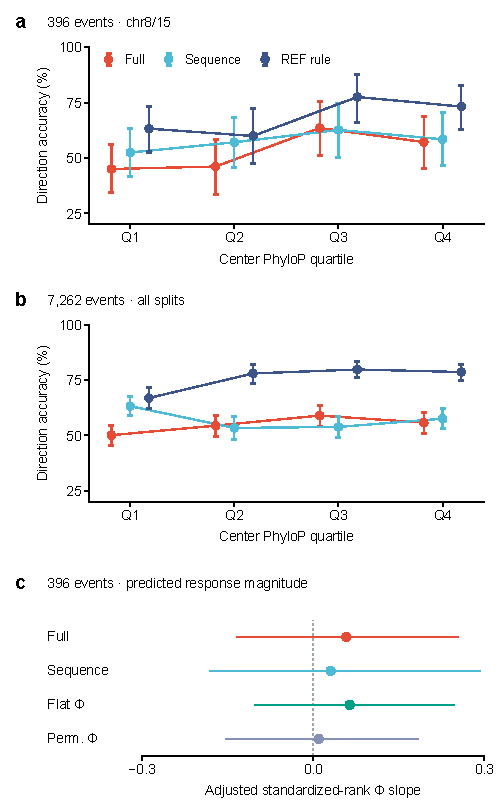
\includegraphics[width=118mm]{figS23_variant_conservation.pdf}
\caption{Conservation strata and predicted perturbation magnitude. RBP-equal direction accuracy for Full, Sequence and the constant REF rule across center-PhyloP quartiles in \textbf{a}, all 396 chromosome-8/15 events and \textbf{b}, the complete 7,262-event development-exposed cohort. Quartiles use unique loci separately per cohort and retain tied scores together; bars give 95\% RBP bootstrap intervals. Unequal event/RBP coverage is retained in Data S25. \textbf{c}, Adjusted standardized-rank slopes for absolute predicted allele-paired log-total-count differences in the chromosome-8/15 cohort, with approximate two-way region/RBP multiplier intervals. These are predicted-magnitude associations, not measured binding-effect correlations. Full-refit/region sensitivities and all controls remain in Data S25.}
\label{figsupp:variant_conservation}\end{figure}

\clearpage
\begin{figure}[p]\centering
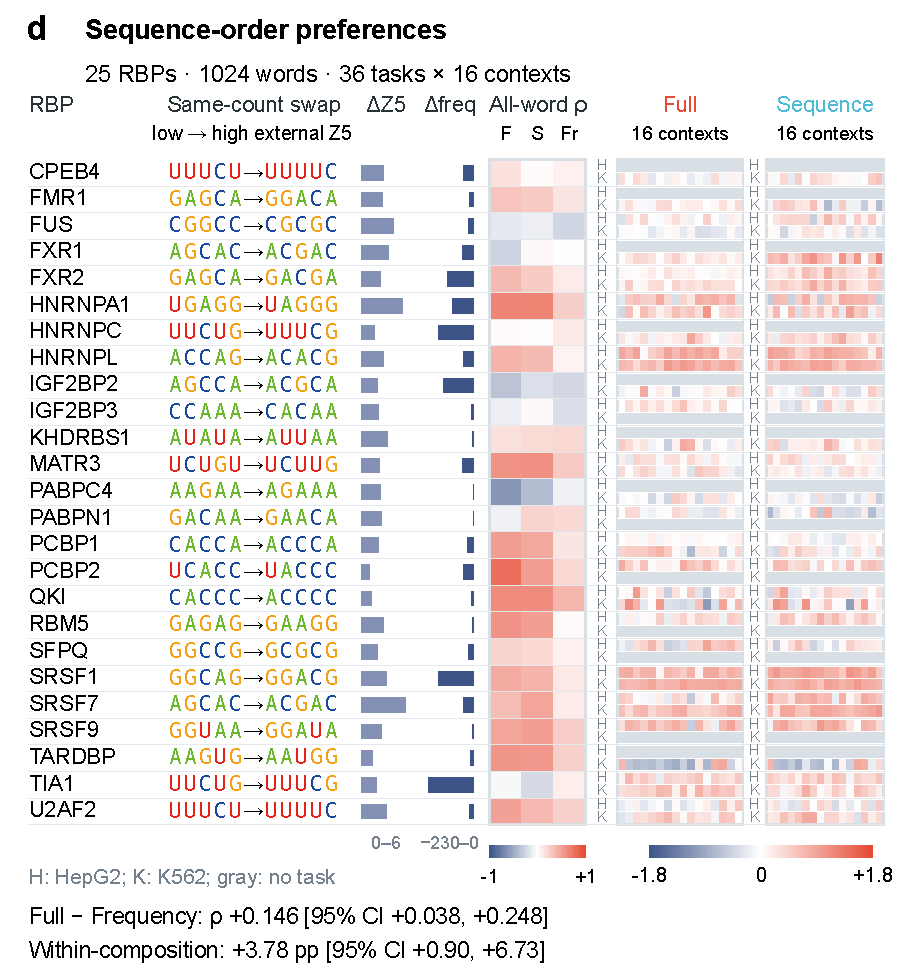
\includegraphics[width=155mm]{figS24_external_edit_atlas.pdf}
\caption{Expanded complete external-first edit atlas retained from the previous Figure~5. All 25 proteins remain in frozen order, with composition-preserving low-to-high external-preference edits, independent RNAcompete-derived $\Delta Z_5$, native-frequency changes, primary all-word Spearman estimates and all 1,152 Full/Sequence model-background responses across 36 tasks. H/K identify HepG2/K562; grey cells indicate unavailable tasks. Positive responses favour the externally preferred word. Response cells retain the archived zero-centred asinh colour mapping in original log-count units. Frozen primary/secondary estimates and paired-protein contrasts are unchanged. Backgrounds are computational, and word preference is not a measured effect of the hypothetical edits in native transcripts. The archived panel letter d identifies this former population-edit atlas; current Figure~5a retains the complete primary and secondary endpoint differences from Frequency. QKI's CACCC$\to$ACCCC edit here differs from the complete A$_2$C$_2$U group in Figure~5b/S26; the HNRNPA1 edit matches Figure~S28c. See S1.18 and Data S23.}
\label{figsupp:external_edit_atlas}\end{figure}

\clearpage
\begin{figure}[p]\centering
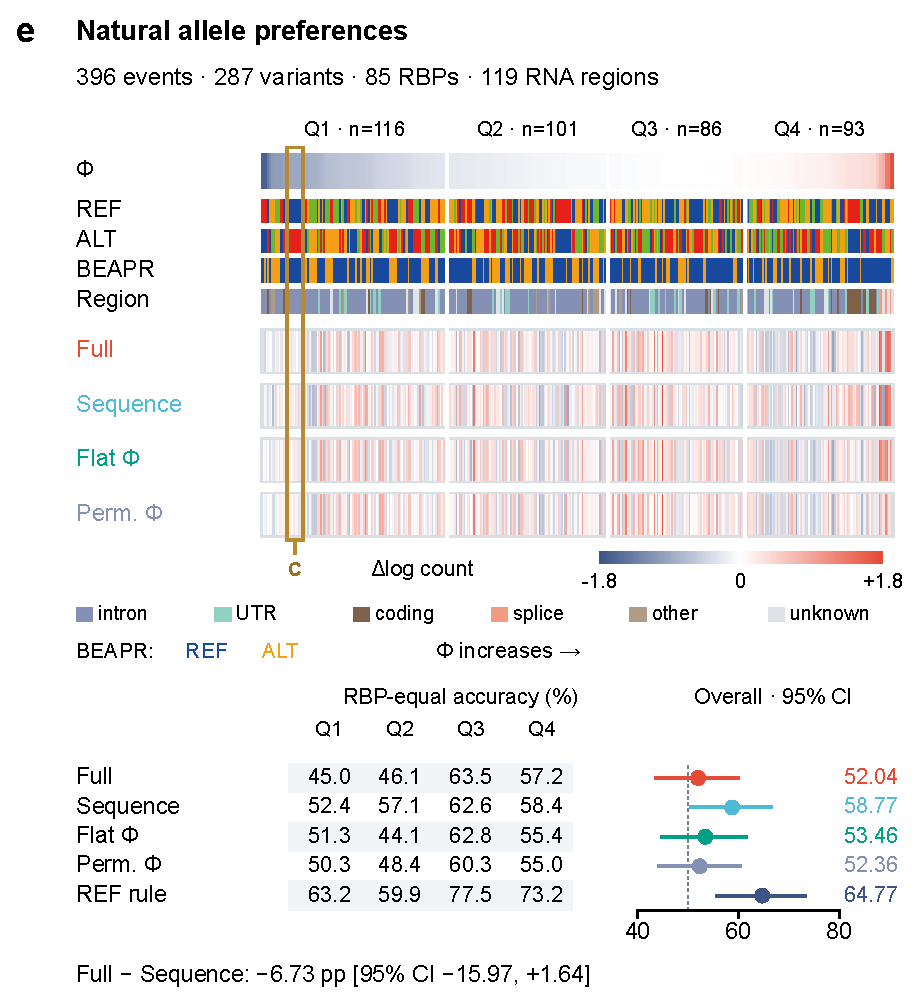
\includegraphics[width=155mm]{figS25_natural_event_atlas.pdf}
\caption{Expanded complete natural-event atlas retained from the previous Figure~5. All 396 events at 287 variants, spanning 85 RBPs and 119 RNA regions, are sorted by centre PhyloP and event identity without prediction success. PhyloP, genomic REF/ALT identity, BEAPR-preferred allele, genomic region and four predicted preferred-minus-other responses share exact columns. Outlined columns locate the ten-event coverage-first C$>$T example, shown in Figure~S28e; the archived artwork retains its original panel c label. All five-arm quartile summaries remain; overall intervals use two-way RNA-region/RBP multipliers. REF/ALT and region tracks are annotations, not independent binding or pathogenicity measurements. The ASB-positive cohort was previously exposed and evaluates direction conditional on ASB. No overall conservation-specific interpretation advantage is established. Current Figure~5d retains all Full/Sequence event responses and aggregate accuracy; Figure~S28f retains the adjusted Full slopes. See S1.20 and Data S25.}
\label{figsupp:natural_event_atlas}\end{figure}

\clearpage
\begin{figure}[p]\centering
\captionsetup{font=qkicompact}
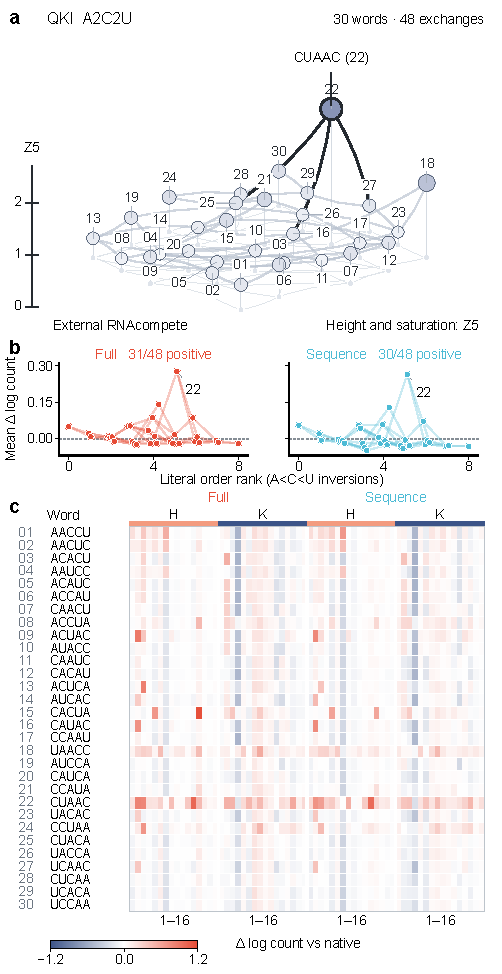
\includegraphics[width=85mm]{figS26.pdf}
\caption{Complete fixed-composition QKI sequence landscape and matched predictive contexts, from the previously explored B2 source. \textbf{a}, All 30 literal A$_2$C$_2$U five-mers and all 48 adjacent exchanges of different nucleotides. IDs 01--30 decode in c; CUAAC is node 22. The pale base follows A$<$C$<$U inversion rank and lexical within-rank order. Stems link raised and identical base nodes. Height, area and saturation encode assay-mean RNAcompete $Z_5$ on a common linear scale. CUAAC's three neighbouring edges are outlined; width does not encode interactions. \textbf{b}, All 30 nodes and 48 edges projected onto Full and Sequence mean replacement-minus-native log-count responses across the same 32 backgrounds. Axes are literal inversion rank and predicted response. Edges oriented towards higher external $Z_5$ have positive mean contrasts in 31/48 Full and 30/48 Sequence edges; weak and adverse edges remain. \textbf{c}, Every saved response for 30 words across 32 fixed native 101-nt contexts in each arm (1,920 values), aligned by exact word and node ID. H/K denote HepG2/K562, each retaining its original 16-background order. Both matrices share the absolute linear $[-1.2,+1.2]$ scale. RNAcompete $Z_5$ averages every contributing seven-mer occurrence, then averages same-protein assays equally; it is not measured binding in the edited native windows. Replacements occupy positions 49--53 with original Full $\Phi$ fixed. The base is literal sequence topology, not a learned embedding, RNA structure or fitness landscape; adjacent swaps are not epistasis or learned interactions. Backgrounds are computational inputs. Matched training histories are unverified, and no conservation effect or general Full superiority is established. The unchanged TIA1 five-word/four-edge boundary results remain in Data S23. No new training, inference, bootstrap or $p$ values were generated. See S1.18 and Figure~5b.}
\label{figsupp:qki_complete_graph}\end{figure}

\clearpage
\begin{figure}[p]
\centering
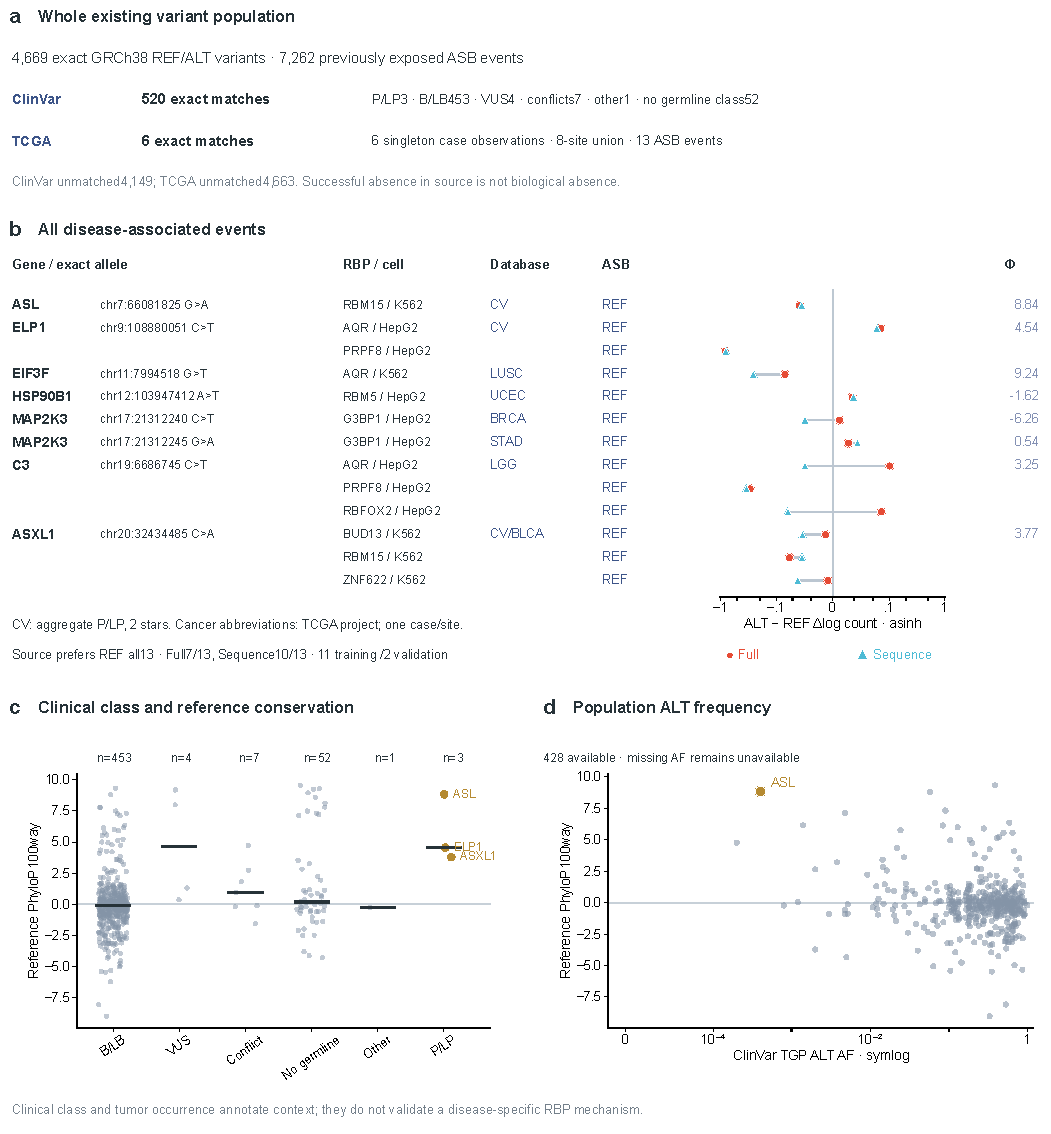
\includegraphics[width=160mm]{figS27.pdf}
\caption{Exact clinical/tumor annotations and conservation context. \textbf{a}, Complete 4,669-variant coverage: 520 exact ClinVar matches and six exact open TCGA matches; unannotated is distinct from benign. \textbf{b}, All 13 ASB events at the eight-variant union, with exact allele, RBP/cell, clinical/cancer flags, measured REF preference and Full/Sequence ALT-minus-REF response on one asinh axis (linear width 0.02). Eleven events are from training chromosomes and two from validation chromosomes. CV denotes aggregate P/LP with two-star review; cancer abbreviations identify TCGA projects, each with one case at the displayed site. \textbf{c}, All 520 unique ClinVar variants' reference PhyloP by aggregate germline class. Every variant is shown; black bars are descriptive medians, and three P/LP sites are named. \textbf{d}, All 428 returned current ClinVar TGP ALT frequencies versus reference PhyloP, using symlog with linear threshold $10^{-4}$. Explicit source zero is plotted; unavailable AF remains missing. ASL is the sole P/LP site with returned TGP AF. These descriptive annotations do not establish class-discrimination performance, clinical causality or mutant conservation. Complete sources, conditions, source-specific AF and event identities: S1.21, Data S26.}
\label{fig:s27_disease}
\end{figure}
\clearpage

\clearpage
\begin{figure}[p]
\centering
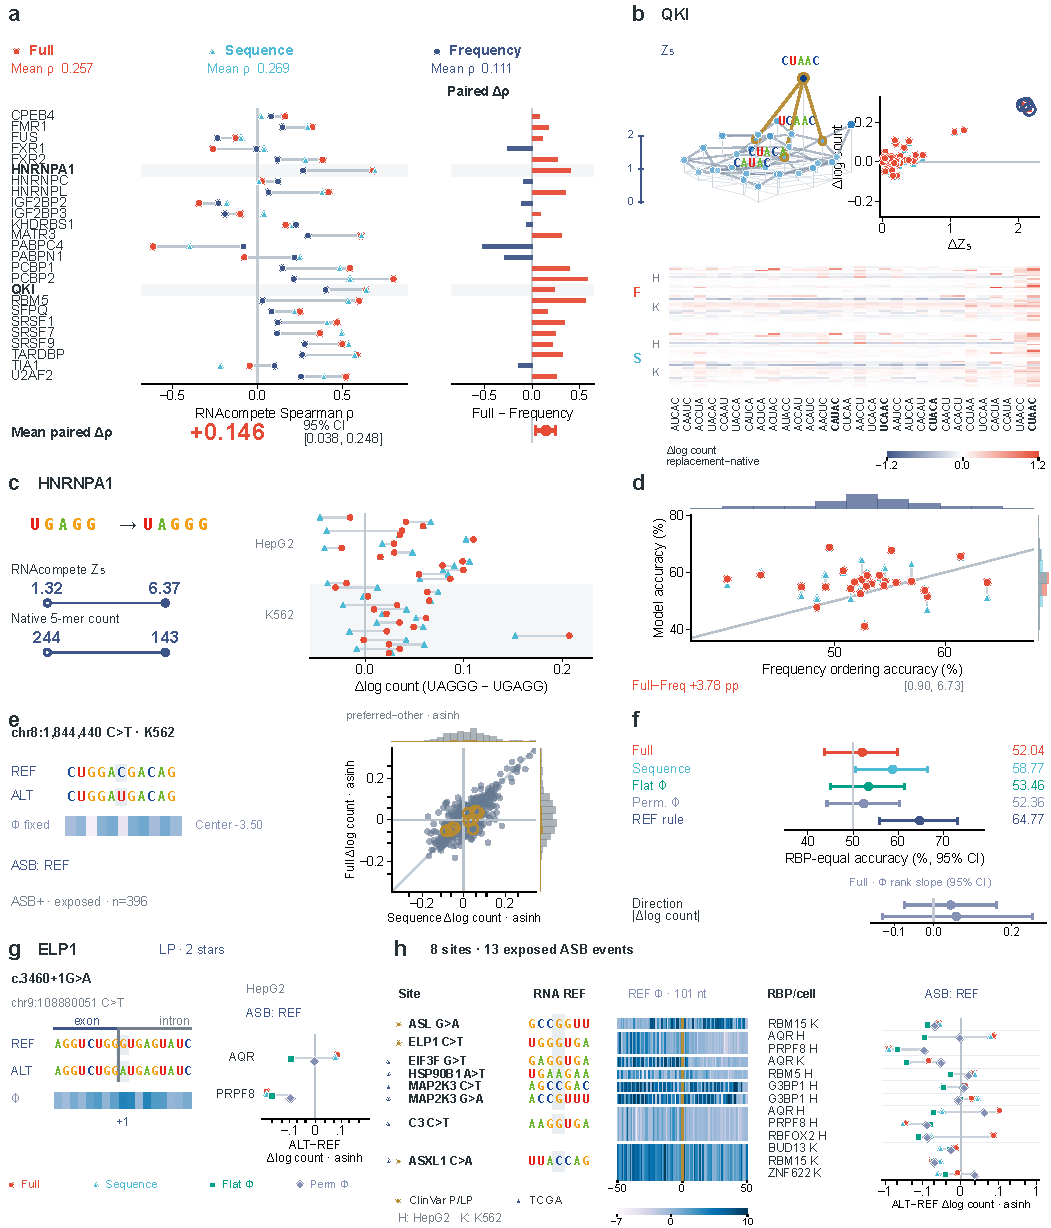
\includegraphics[width=160mm]{figS28.pdf}
\caption{Complete external-preference, natural-allele and clinical-context displays. \textbf{a}, All 25 primary protein scores and Full-minus-Frequency contrasts. \textbf{b}, QKI's complete 30-word/48-exchange landscape, 48 mean contrasts and both 32-background/30-word matrices. \textbf{c}, HNRNPA1 edit and paired backgrounds. \textbf{d}, Secondary composition-matched concordance. \textbf{e}, Native alleles, fixed reference $\Phi$ and all 396 exposed ASB-positive responses; ten locus events outlined. \textbf{f}, Five-arm accuracy and adjusted Full $\Phi$ slopes; both slope intervals cross zero. \textbf{g}, ELP1 donor and AQR/PRPF8 events, including AQR failure. \textbf{h}, All eight clinical/tumor sites and 13 events: RNA cores, reference $\Phi$ and four ALT-minus-REF responses. Flat/permuted controls use fixed Full weights. Clinical annotations are not binding labels; the cohort was exposed. Methods S1.18/S1.20/S1.21; Data S23/S25/S26.}
\label{fig:s28}
\end{figure}
\clearpage

\clearpage
\begin{figure}[p]\centering
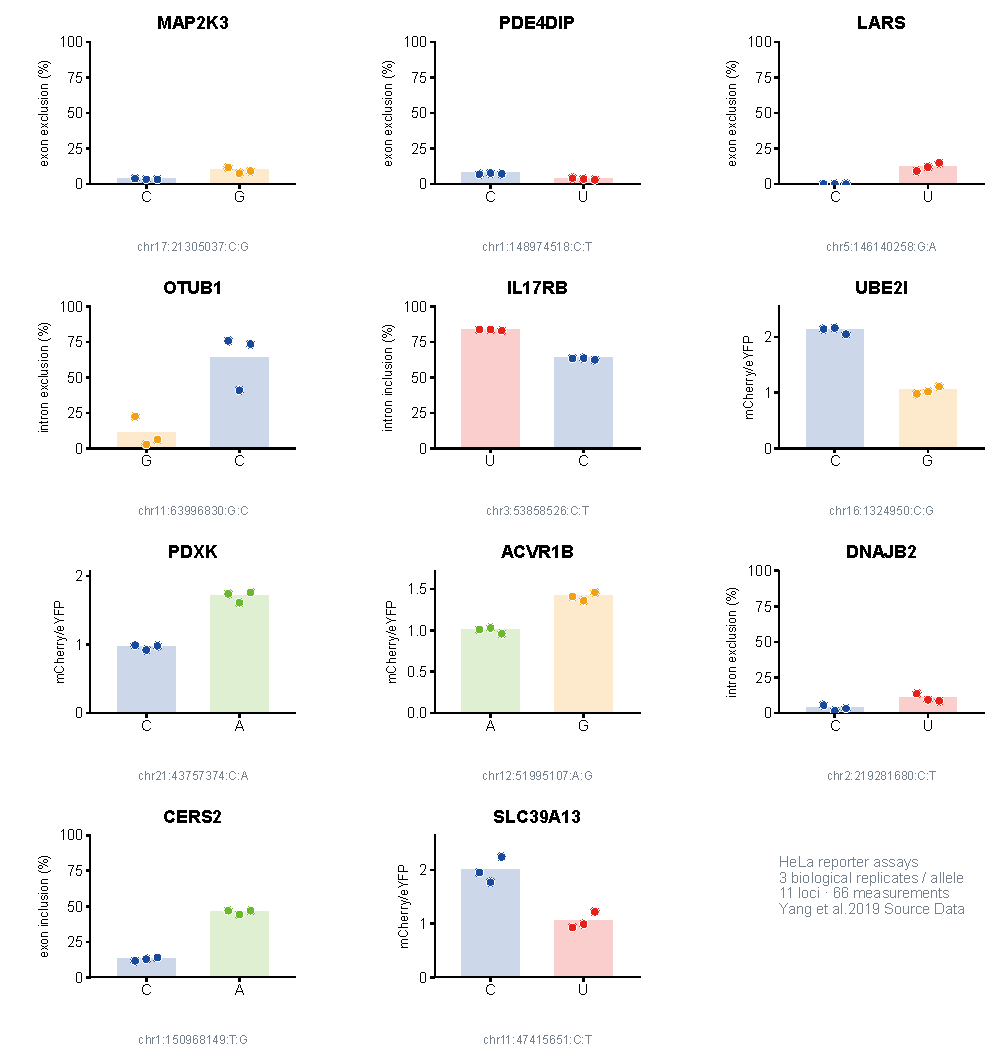
\includegraphics[width=160mm]{figS29_reporter_measurements.pdf}
\caption{Complete author-measured reporter outcomes at all eleven exact natural-variant sites. Each plot retains both RNA alleles and all three source biological replicates, with descriptive means. Exon/intron inclusion or exclusion remains on the original percentage scale; mCherry/eYFP remains the original normalized expression ratio. All assays were performed by \citet{yang2019asb} in HeLa, rather than generated here. These are measured regulatory phenotypes, not CARBON predictions. Exact input/primer matching, the explicitly inferred UBE2I alternative primer and the SCL39A13 source-label correction are in S1.22 and Data S27. The author-selected reporter population was exposed and contains no new blind confirmation sample.}
\label{fig:s29_reporter}\end{figure}
\clearpage
\begin{figure}[p]\centering
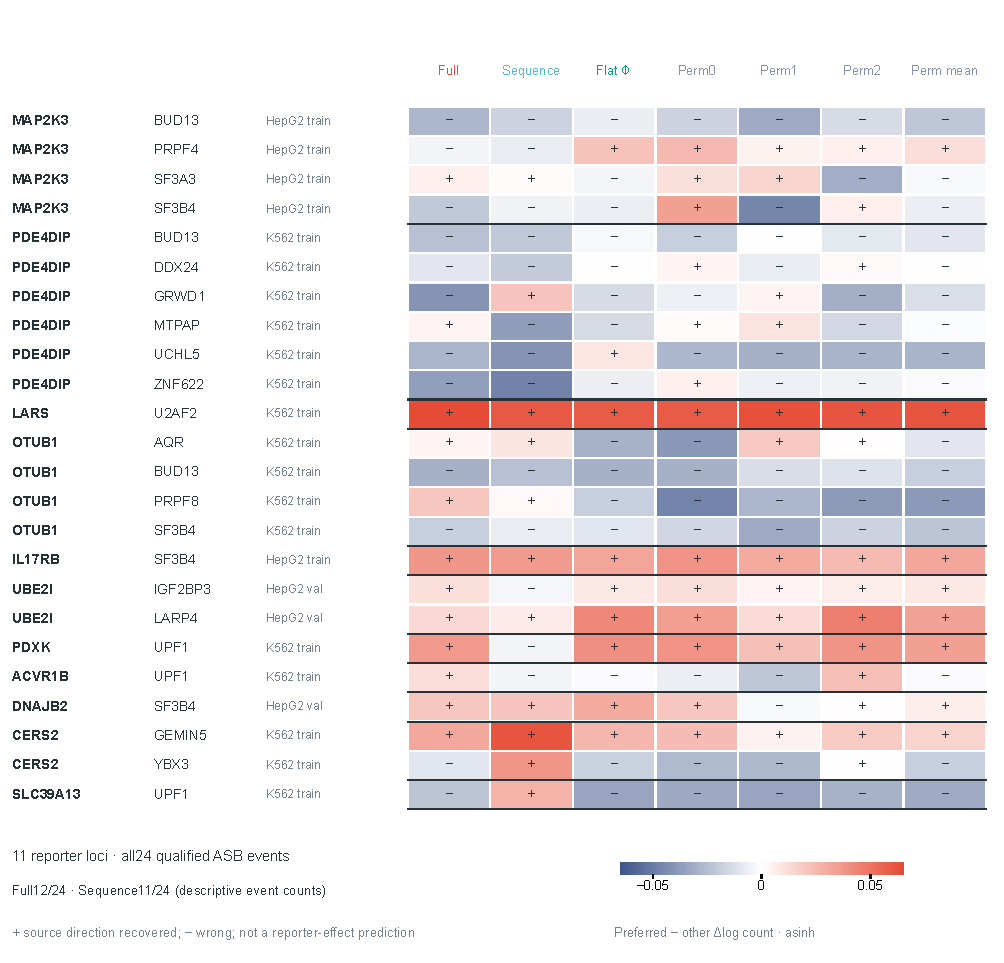
\includegraphics[width=160mm]{figS30_reporter_binding.pdf}
\caption{Every qualified ASB event at all eleven reporter loci. All 24 RBP/cell events and all seven frozen prediction/input-control arms are retained, including failures and individual conservation permutations. Colour encodes preferred-minus-other log-count difference on one symmetric asinh scale (linear width 0.02); + denotes the source-preferred direction and minus denotes the opposite. The letters do not encode a predicted reporter-expression or splicing direction. All source labels and model outputs were exposed; 21 events are on training chromosomes and three on validation chromosomes. The Full 12/24 versus Sequence 11/24 counts are descriptive, not a general model advantage or a new significance test. Same-site RBP observations are not independent variant or patient replicates. All source reporter outcomes remain in S29, with identities, exact primer checks, unsuccessful candidates and selection in S1.22/Data S27.}
\label{fig:s30_reporter_binding}\end{figure}
\clearpage
\clearpage
\begin{figure}[p]\centering
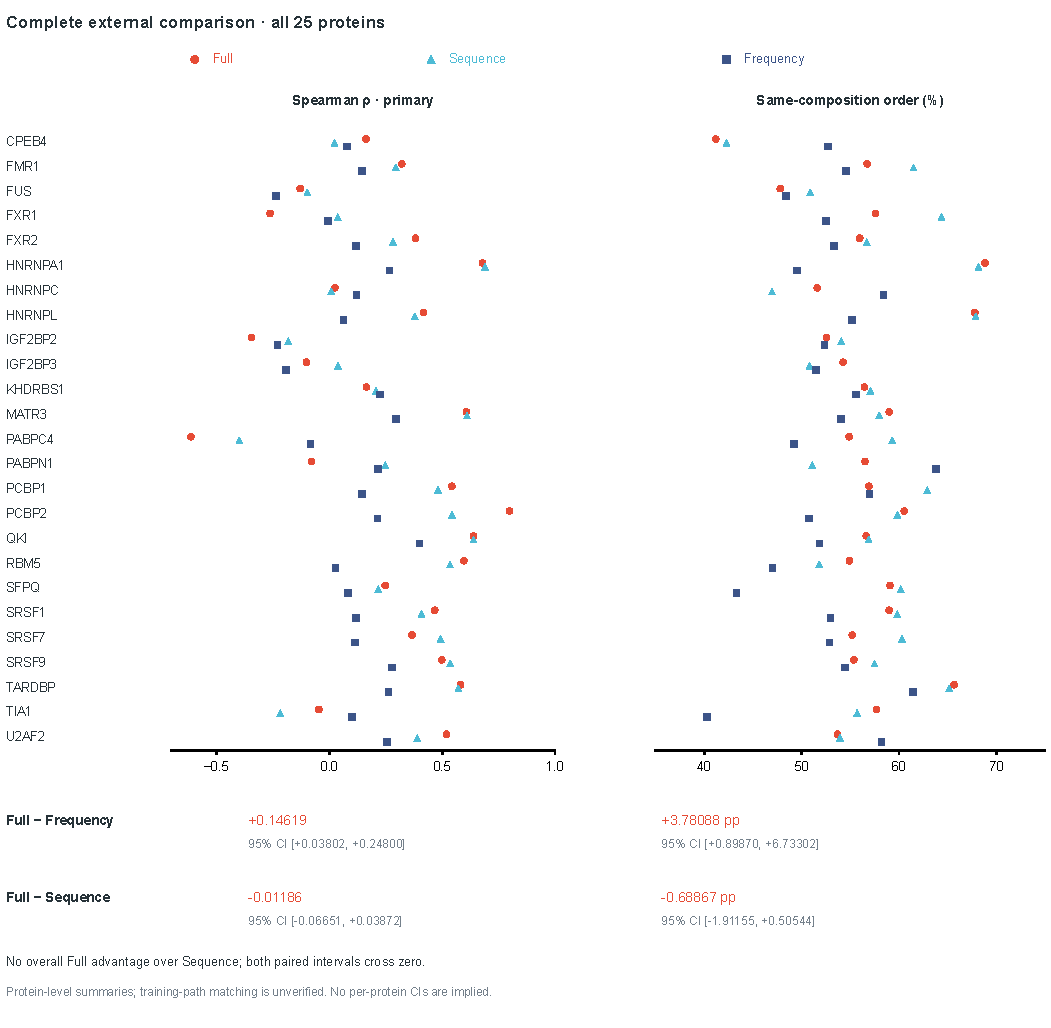
\includegraphics[width=160mm]{figS31_sequence_complete.pdf}
\caption{Complete external-preference comparison retained alongside main Figure~5a. All 25 proteins, Full/Sequence/Frequency arms, primary all-word Spearman and secondary composition-matched concordance are retained. The displayed original paired-protein contrasts and 95\% intervals use the frozen protein resamples; they are not derived from the axis geometry. The Full-minus-Sequence contrasts are $-0.01186$ [$-0.06651$, $0.03872$] Spearman and $-0.68867$ [$-1.91155$, $0.50544$] percentage points in concordance, without an overall Full advantage. Training histories are not verified as matched, and these differences cannot isolate conservation. This artwork is byte-identical to the accepted candidate's complete control. Protocol: S1.18; data: S23.}
\label{fig:s31_sequence_complete}\end{figure}
\clearpage
\begin{figure}[p]\centering
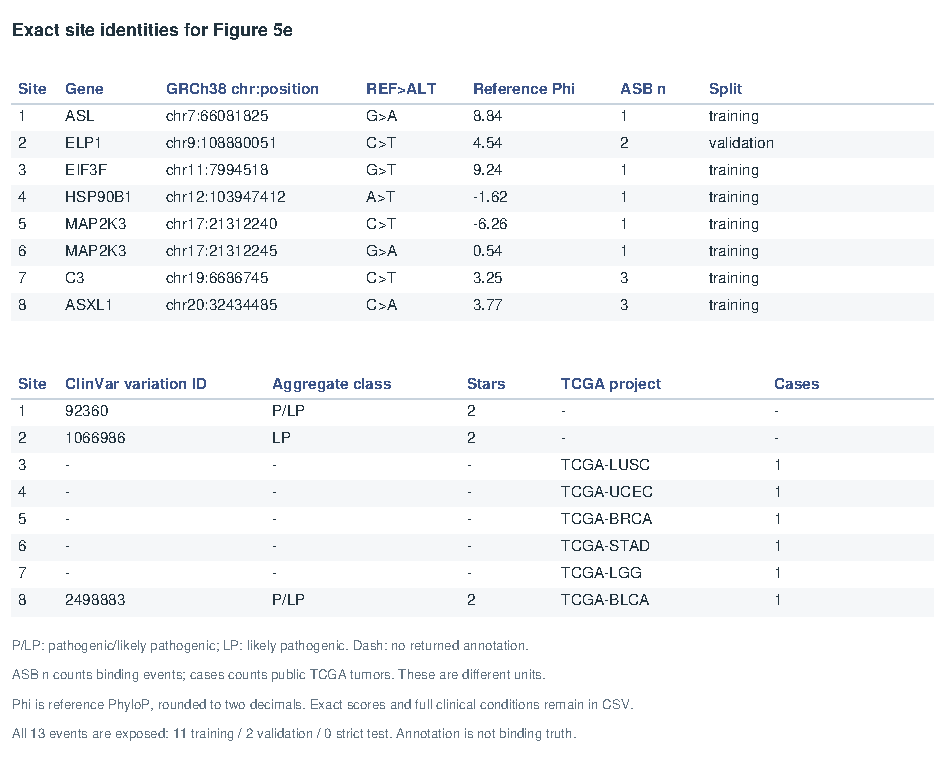
\includegraphics[width=160mm]{figS32_exact_site_index.pdf}
\caption{Exact identities for all eight clinical/tumor-overlap sites in main Figure~5e. Display IDs 1--8 follow the frozen site order and link gene/REF$>$ALT labels to GRCh38 coordinates, ClinVar IDs and aggregate classes, TCGA projects, source ASB-event counts, training/validation split and focal reference PhyloP. The two aligned blocks retain all eight frozen site identities and database annotations. Reference PhyloP is rounded to two decimals; exact values and full reported conditions remain in the CSV. ASB counts are binding observations, not patients. Every TCGA-overlap site has one public tumor case. There are no strict-test events, and database annotation is not an independent binding or disease-mechanism measurement. Exact CSV: \texttt{CLINICAL\_SITE\_INDEX.csv}; complete records: Data S26.}
\label{fig:s32_exact_site_index}\end{figure}
\clearpage
\clearpage\section{Supplementary Data}

Data S1--S14 are provided in \path{source_data/S1_S14_original/}; later directories are listed below. S21 contains the limited training-seed sensitivity check. S22/S23 contain the complete allocation and external-preference packages. Availability is described in S1.10.


\footnotesize

\begin{longtable}{@{}>{\raggedright\arraybackslash}p{0.07\linewidth}>{\raggedright\arraybackslash}p{0.43\linewidth}>{\raggedright\arraybackslash}p{0.43\linewidth}@{}}
\toprule
Item & File & Content \\
\midrule
\endfirsthead
\toprule
Item & File (continued) & Content \\
\midrule
\endhead

S1 & \path{Supplementary_Data_S1_benchmark_metrics.csv} & Archived implementation-specific metrics for 222 task names; comparison limitations in S1.3. \\
S2 & \path{Supplementary_Data_S2_ablation_paired_deltas.csv} & Paired per-task deltas between the retained full configuration and each ablated configuration. \\
S3 & \path{Supplementary_Data_S3_comparator_win_loss_matrix.csv} & Archived paired comparison signs; limitations in S1.3. \\
S4 & \path{Supplementary_Data_S4_cross_cell_complete_score_set.tsv} & Unfiltered cross-cell table (146 records); restriction to K562 and HepG2 gives 140 records and 70 symbols. \\
S5 & \path{Supplementary_Data_S5_cross_cell_overlap_join_128.tsv} & Peak-overlap inner join used for the Jaccard analyses: 64 symbols, 128 directional records. \\
S6 & \path{Supplementary_Data_S6_motif_comparisons.csv} & Aligned attribution-derived pattern comparisons, 193 comparisons, including 72 with $q<0.05$. \\
S7 & \path{Supplementary_Data_S7_conservation_task_summary.csv} & Task-level peak and within-window non-peak conservation summaries used for Figure~S12a. \\
S8 & \path{Supplementary_Data_S8_conservation_bin_summary.csv} & Task--bin summaries underlying Figures~S6/S9d--f and Figure~S3b--d, including derived Q4-minus-Q1 contrasts. \\
S9 & \path{Supplementary_Data_S9_conservation_peak_centred_profile.csv} & Per-offset mean PhyloP for the 12{,}000 peak-centred profiles and their within-window control positions, with bootstrap 95\% bounds plotted in Figure~S12a and Figure~S3a. \\
S10 & \path{Supplementary_Data_S10_motif_leaf_mapping.csv} & Mapping of 219 overview leaves to task, pattern~0 crop, functional/domain annotations and S6 cognate comparisons. \\
S11 & \path{Supplementary_Data_S11_conservation_perturbation.csv} & Primary and control paired effects and sample sizes for all 222 tasks. \\
S12 & \path{Supplementary_Data_S12_RBP_robustness.csv} & 4,800 RBP-level conservation rows spanning two strata, four quartiles and four metrics. \\
S13 & \path{Supplementary_Data_S13_perturbation_condition_metrics.csv} & 3,330 task--condition correlation and Signal AP records from frozen-model inference. \\
S14 & \path{Supplementary_Data_S14_count_inverse_sensitivity.csv} & Per-task metric changes from the numerical inverse-count correction on the sampled windows. \\
S15 & \path{source_data/S15_conditional_conservation/} & All paired RBP contrasts, row summaries, curves and display order for Figure~S12c. \\
S16 & \path{source_data/S16_motif_instances/} & Fixed aligned PPM/CWM/PhyloP arrays, all instance tracks and complete motif population contrasts. \\
S17 & \path{source_data/S17_factorial/} & All 1,120 windows, 140 task summaries, 70 RBP summaries and frozen aggregate results. \\
S18 & \path{source_data/S18_fixed_cases/} & Both saved case tensors and the exact block/conditional-substitution values in Figure~S13a,b. \\
S19 & \path{source_data/S19_ASB/} & All 396 event predictions, source labels, task/RBP summaries, sensitivities and provenance records. \\
S20 & \path{source_data/S20_benchmark_annotations/} & All scatter extrema, task-paired benchmark values and the signed Figure~2g matrix. \\
S21 & \path{source_data/S21_seed_sensitivity/} & Two-task three-seed sensitivity summaries, training metadata and array-level verification. \\

S22 & \path{source_data/S22_context_allocation/} & Native repeated-core identities, all model/gene/seed endpoints, bootstrap summaries, manifests, post hoc selection, native arrays and Fig.~4 sources. \\
S23 & \path{source_data/S23_external_order_preferences/} & External measured-score metadata, original primary/secondary endpoints, complete controls/candidates, native backgrounds and Fig.~5 intervention records. \\
S24 & \path{source_data/S24_motif_reference_audit/} & All 193 original CISBP comparisons and exact source metadata; complete ATtRACT snapshot, 485-query Tomtom run, cognate coverage, display selection and aligned matrices. \\
S25 & \path{source_data/S25_natural_variants/} & All 7,262 exposed ASB events, the complete 396-event subset, exact allele annotations/failures, frozen inputs/predictions, direction and conservation analyses, code and source hashes. \\
S26 & \path{source_data/S26_disease_annotations/} & Whole-cohort exact ClinVar/TCGA statuses, direct clinical records, complete 8-site/13-event union, source-specific population AF, conservation context and reproducible descriptive code. \\


S27 & \path{source_data/S27_reporter_validation/} & All eleven exact reporter loci,24 ASB events,66 author biological measurements, source workbooks/primers, allele mapping, all seven model/control responses and exploratory case-selection records. \\
\bottomrule
\end{longtable}


\noindent Staged access and licence status are described in S1.10; public availability is not asserted.

\clearpage\normalsize

\bibliographystyle{carbon-oup-abbrvnat}
\bibliography{reference}
\end{document}
